\tolerance=10000

\documentclass[12pt]{report}
\usepackage{graphicx}

%This package is built on the LaTeX2e report class, so any other packages which are
%also compatible with it can also be used in combination with it.  ODUthesis should
%be in the directory in which you are working, or in one of the standard input directories
%for the TeX installation on your system.

\usepackage{amsmath}
\usepackage{float}
\usepackage{gensymb}
\usepackage{url}
\usepackage{feynmp-auto}
\usepackage{hyperref}
\usepackage{amssymb}

%This package causes the first line of a section to be indented as required by the dissertation guide.

\usepackage{indentfirst}
\usepackage{booktabs}

%%%%%Other LaTeX2e packages such as the AMS fonts and graphics packages can be included here.

%This style follows conventions used in Physical Review C. The names of figures, tables and captions can
%be changed by using the commands below with appropriate changes. For example, "FIG." could be replaced by
%"Fig." or "Figure" to change the labeling of figure captions.

%\renewcommand{\figurename}{FIG.}
%\renewcommand{\tablename}{TABLE}
%\renewcommand{\bibname}{BIBLIOGRAPHY}

\usepackage{chngcntr}
\usepackage{ODUthesis}

\counterwithin{figure}{section}

%\counterwithin{equation}{section}

\begin{document}

\title{Searching for Heavy Photons with Detached Vertices in the Heavy Photon Search Experiment}

\author{Holly Szumila-Vance}
\principaladviser{Lawrence Weinstein}
\member{John Adam}
\member{J. W. Van Orden}
\member{Stepan Stepanyan}  %This command produces a signature line for the specified member on the
\member{Leposava Vuskovic}  %title page. Use on instance of this command for each member of the
                   %committee other than the advisor up to a total of 5 members.

\degrees{B.S. May 2008, Embry-Riddle Aeronautical University \\ B.S. May 2009, Embry-Riddle Aeronautical University \\ M.S. May 2014, Old Dominion University}


\dept{Physics}          %for example \dept{physics}

\submitdate{June 2017}

%\phdfalse          %produces language on title page for Masters Thesis. Otherwise the default
                    %is for a Ph.D. dissertation.

%\copyrightfalse    %suppresses copyright notice

%\figurespagefalse  %suppresses List of Figures

%\tablespagefalse   %suppresses List of Tables

\vita{
\textbf{}\\
\textbf{Education:}\\ 
\\
Old Dominion University, Norfolk, VA\\
\begin{itemize}
\item PhD Candidate in experimental nuclear physics, 2012--2017\\
\item Master of Science, 2014\\
\end{itemize}
Embry--Riddle Aeronautical University, Prescott, AZ\\
\begin{itemize}
\item Bachelor of Science in Aerospace Engineering, 2009\\
\item Bachelor of Science in Space Physics, 2008\\
\end{itemize}
\textbf{Research Experience:}\\
\begin{itemize}
\item 2013--2017, graduate research assistant searching for heavy photons in the Heavy Photon Search experiment at Jefferson Lab, Hall B\\
\item 2013, graduate research assistant testing CLAS12 Region II drift chambers at the Old Dominion University clean room\\
\end{itemize}
\textbf{Publications:}\\
\begin{itemize}
\item N. Baltzell, et al, ``The HPS beamline and its performance", Nucl. Inst. And Meth. A, in press; https://arxiv.org/pdf/1612.07821.pdf\\
\item I. Balossino, et al.,``The HPS electromagnetic calorimeter”, Nucl. Inst. And Meth. A, in press;
https://arxiv.org/pdf/1610.04319v2.pdf\\
%\item (Internal note) ``HPS/ECal simulations: energy and position reconstruction for electrons, positrons, and photons": https://misportal.jlab.org/mis/physics/hps_notes/viewFile.cfm/2014-001.pdf?documentId=1\\
%\item (Internal note) ``Ecal Timing Calibration for the Spring 2015 Engineering Run": https://misportal.jlab.org/mis/physics/hps_notes/viewFile.cfm/2015-011.pdf?documentId=13\\
%\item (Internal note) ``HPS Energy Calibration for the Spring 2015 Engineering Run": https://misportal.jlab.org/mis/physics/hps_notes/viewFile.cfm/2016-002.pdf?documentId=18\\
\end{itemize}
\textbf{Previous Work Experience:}\\
\begin{itemize}
\item Old Dominion University: Astronomy teaching assistant\\
\item Virginia Army National Guard: Assistant S-3, operations officer\\
\item Arizona Army National Guard: MEDEVAC platoon leader\\
\item Center for Space Nuclear Research, research internship\\
\end{itemize}
 }
\abstract{The Jefferson Lab Heavy Photon Search (HPS) experiment is searching for a hypothetical massive particle called the heavy photon which could mediate a dark electromagnetic-type force. If heavy photons kinetically mix with Standard Model photons, they may be radiated by electrons scattering from a heavy nucleus and then decay to $e^+e^-$ pairs. HPS uniquely searches for heavy photons that either decay at the target or a measurable distance after. The experiment utilizes a silicon vertex tracker (SVT) for momentum and vertex reconstruction, together with an electromagnetic calorimeter for measuring particle energies and triggering events. The HPS experiment took its first data during the spring 2015 engineering run using a 1~GeV electron beam incident on a tungsten target and its second data in the spring of 2016 at a beam energy of 2.3 GeV. The 2015 run obtained two days of production data that was used for the first physics results. The analysis of the data was conducted as a blinded analysis by tuning cuts on 10$\%$ of the data.\\
\indent This dissertation discusses the displaced vertex search for heavy photons in the 2015 engineering run. It describes the theoretical motivation for looking for heavy photons and provides an overview of the HPS experimental design and performance. The performance details of the experiment are primarily derived from the 2015 engineering run with some discussion from the higher energy running in 2016. \\
\indent This dissertation further discusses the cuts used to optimize the displaced vertex search and the results of the search. The displaced vertex search did not set a limit on the heavy photon but did validate the methodology for conducting the search. Finally, we used the full data set to make projections and guide future analyses.}
\beforepreface

\prefacesection{Acknowledgments} 
Thank you to everyone who has influenced my life and scientific development during this time. This dissertation would not have been possible without the incredible mentors and colleagues I have had the pleasure to work with. Thank to you all of my HPS collaborators for building and running a successful experiment. Thank you to the Old Dominion University Physics Department for investing so much time creating a positive and stimulating environment for budding physicists.\\
\indent I would like to especially thank Larry Weinstein for being an outstanding advisor and for giving me room to explore in my research while using every opportunity to simplify and clarify new concepts. I thank Stepan Stepanyan for his guidance and direction of the HPS experiment and for organizing a supportive network at Jefferson Lab for conducting physics analysis. I also thank John Jaros for always asking questions and keeping my work relevant. Merci to Michel Gar\c con for teaching me the details of calorimetry as well as the value of a well-written analysis note. 
I thank Nathan Baltzell and Rafayel Paremuzyan for always taking the time to answer my questions and offering advice and guidance on my research. I also especially thank my collaborators at Orsay and INFN with whom I shared the exciting experience of testing and assembling a calorimeter.\\ 
\indent And finally, I thank my family and friends for their unwavering support. I thank my father for instilling in me a curiosity for the universe and the patience needed to understand complex problems. I thank my mother for giving me the gift of communication and expression through words and the perpetual drive to always move forward. I thank my brother for his support and thoughtful discussions about life as a student and scientist- may this dissertation prove that graduate school really does eventually end, (and it is actually only the beginning).\\   
\indent This dissertation is dedicated to my loving husband and best friend, Jeff, for always believing in me and supporting me in everything I do.

    %text of Acknowledgments goes here
    %any other preface section is inserted similarly by the command
    %\prefacesection{Section Title}

\afterpreface

    %The text of the thesis/dissertation begins here. The basic organization is
    %in chapters, sections, subsections. 

\chapter{Introduction}
The heavy photon, also known as the $A^{\prime}$, is a theoretically motivated massive gauge boson that is associated with a predicted U(1) hidden symmetry, favorable to Beyond Standard Model theories. According to theory~\cite{holdom_two_1986}, a heavy photon kinetically mixes with the Standard Model photon through a loop-level effect generating an effective coupling to electric charge. The relative size of this coupling to electric charge, $\epsilon$, can range from $10^{-12}$ to $10^{-2}$ depending on the loop order of the mixing interaction and describes the coupling of the heavy photon to electric charge to be at a scale significantly smaller than that in standard electrodynamic theory. While the coupling strength of the interaction can be naturally generated from the loop interactions, the mass is somewhat less constrained. Theories of the heavy photon as a way to explain cosmological phenomena make them the simplest and possibly leading interaction between the Standard Model and the Dark Sector. The Dark Sector encompasses both dark matter and dark energy particles that do not interact other than gravitationally. If the heavy photon obtains its mass through the Higgs mechanism, the mass is favored to be in the range of MeV to GeV which is compatible with dark matter theories. In such a scenario, electrons could radiate heavy photons as they do ordinary photons but at a suppressed rate. These heavy photons will have measurable lifetimes before decaying to charged particle pairs. It is natural to describe the heavy photon parameter space in terms of its coupling, $\epsilon^2$, and mass, $m_{A'}$.\\
\begin{figure}[htb]
  \centering
      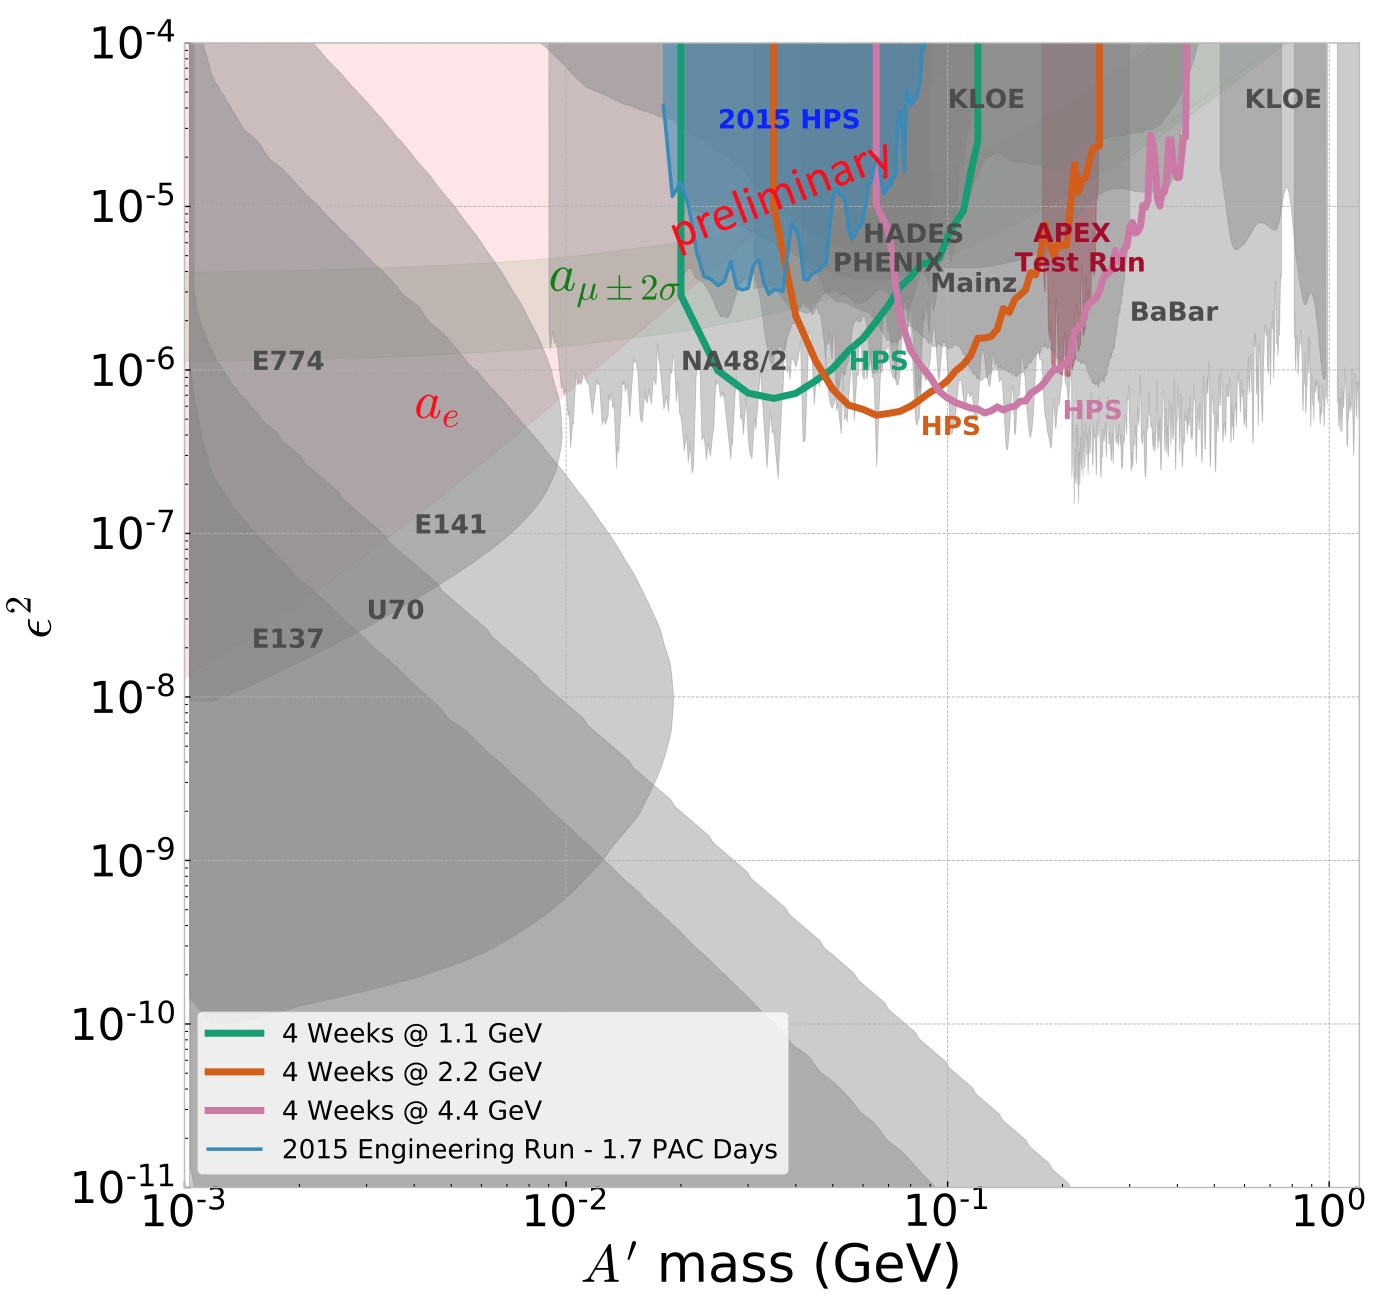
\includegraphics[width=0.7\textwidth]{pics/intro/reach_nominal.png}
  \caption[Reach for the HPS experiment]{The existing 90$\%$ confidence limits from other experiments looking for heavy photons in the relevant mass-coupling region is shown. The shaded blue region includes the preliminary bump hunt results from the 2015 engineering run. The vertex reach is not shown on this plot as no reach is found using the proposed HPS run configuration. The region labeled as $a_\mu$ indicates the favored parameter space for a visibly decaying heavy photon to explain the discrepancy between the calculated and measured muon anomalous magnetic moment. The experiments along the top of the plot with large coupling look for heavy photons that decay promptly at the target. The limits shown in grey along the left side of the plot with decreasing values of coupling look for heavy photons with displaced vertices in beam dump experiments.}
      \label{Figure:projectedReach}
\end{figure}
\indent The Heavy Photon Search (HPS) experiment is searching for heavy photons in the mass range of 20 to 1000~MeV/c$^2$ with prompt or displaced vertices with respect to the target interaction. HPS  generates heavy photons from an electron beam incident on a heavy target and measures the momentum and vertex position of $e^+e^-$ pairs produced from its decay. By reconstructing the invariant mass and the vertex position of the pairs, HPS can look for a small bump on a large background using a bump hunt for prompt decays. Uniquely, HPS is also able to look for heavy photons with smaller couplings (and longer lifetimes) characterized by displaced vertices by searching for a small signal on low background downstream of the target. The HPS reach attained from the 2015 engineering run from the bump hunt is shown in Figure~\ref{Figure:projReach} along with the existing limits from other experiments.\\
\indent The HPS experiment took place in Hall B at the Jefferson Laboratory National Accelerator Facility. The Continuous Electron Beam Accelerator Facility (CEBAF) at Jefferson Lab produces an electron beam that collides with the HPS target material in Hall B. The HPS detector measures the particles from this interaction and searches for the heavy photon signal. The HPS detector consists of a Silicon Vertex Tracker (SVT) and an Electromagnetic Calorimeter (ECal). The SVT measures particle trajectories and reconstructs the vertex position of the particle pair. The ECal triggers event readout in addition to measuring particle energy and pair coincidence timing. \\
\indent The ECal was commissioned during a short commissioning run in December 2014. The full experiment ran in the spring of 2015 commissioning the full beamline and both detectors. This run took 2.3~days of good data at approximately 50~nA with a beam energy of 1.056~GeV. HPS obtained a total of 1529~nb$^{-1}$ of good data. During the commissioning of the SVT, some data was taken with the SVT slightly open from its nominal position before moving the SVT in to its designed position at $\pm0.5$~mm from the beam. A second run in the spring of 2016 used a 200~nA electron beam at 2.3~GeV collecting a total of 5.7~days of data.  Future running at higher electron beam energy is planned for 2018 and beyond.\\
\indent In this dissertation, I describe the search for heavy photons with a displaced vertex using data from the 2015 engineering run. I will describe the experiment as a whole focusing on the areas in which I was most involved. I performed a blinded analysis using 10$\%$ of the data. In order to better understand and analyze the backgrounds in the vertex search, I conducted a further study of the backgrounds using the statistics of the fully unblinded dataset. I will discuss the backgrounds and reach from the Engineering Run.\\
\indent In addition to the full vertex analysis, I contributed significantly to the assembly, characterization and commissioning of the ECal for all experimental running. I wrote the clustering algorithm based on that used by the CLAS experiment Inner Calorimeter (IC) and improved simulations of the ECal detector response. I also calibrated the ECal in both energy and time for both experimental runs. 
%%%%%%%%%%%%%%%%%%%%%%%%%%%%%%%%%%%%%%%%%
\chapter{Motivation} 
The Standard Model (SM) is the most successful theory for describing elementary particles and their interactions via the electromagnetic, strong, and weak forces in terms of gauge theory interactions. The existence of an additional U(1) hidden symmetry is not forbidden by the SM. The heavy photon is the proposed gauge boson for the dark electromagnetic force that would arise from a U(1) broken symmetry. If such an interaction exists, then the SM photon and heavy photon would mix, thus inducing a coupling between the heavy photon and electric charge equal to $\epsilon e$~\cite{holdom_two_1986}. This coupling is significant because electrons could radiate heavy photons similar to radiating SM photons, although at rates decreased by $\epsilon^2$. The primary goal of HPS and many similar experiments is to experimentally detect the heavy photon through this production mechanism. The heavy photon is additionally referred to as the $A^{\prime}$, dark photon, or $U$-boson.

\section{Theory of heavy photons}
The possible existence of a heavy photon rests on the allowable symmetries from the Standard Model. An additional U(1) symmetry in nature could interact with the SM through the mechanism of kinetic mixing~\cite{holdom_two_1986}. Under kinetic mixing, a new gauge boson (heavy photon or $A^{\prime}$) couples to the electromagnetic current through the SM photon by some amount $\epsilon$. Kinetic mixing generates the coupling strength, $\epsilon$, through loop interactions as shown in Figure~\ref{fig:loop}. 

\begin{figure}[htb]
    \begin{center}
        \begin{fmffile}{loop}
            \begin{fmfgraph*}(150,150)
                \fmfstraight 
                \fmfleft{i1}
                \fmfright{o1}
                \fmflabel{$\gamma$}{i1}
                \fmflabel{$A^{\prime}$}{o1}
                \fmf{photon,tension=1}{i1,v1}
                \fmf{photon,tension=1}{v2,o1}
                \fmf{fermion,left,label=$\chi$}{v2,v1}
                \fmf{fermion,left,label=$\chi^{\prime}$}{v1,v2}
            \end{fmfgraph*}
        \end{fmffile}
    \end{center}
    \caption[Kinetic mixing of the SM photon with a heavy photon]{Kinetic mixing of the SM photon with a heavy photon is shown at the one-loop level. $\chi$ can be any massive particle that is charged under both the $A^{\prime}$ and SM U(1) interactions.}
    \label{fig:loop}
\end{figure}

In the simplest scenario, there is one particle $\chi$ that is charged under both the U(1) and new U(1)$^{\prime}$. This single loop level interaction can generate the $\epsilon$ coupling to be in the range of $10^{-4}$ to $10^{-2}$. In Grand Unified Theory (GUT), symmetries forbid one-loop interactions and favor two-loop interactions generating an $\epsilon$ in the range of $10^{-5}$ to $10^{-3}$~\cite{alexander_dark_2016}. If both U(1)s are in unified groups, higher loop interactions generating even smaller couplings are possible. The gauge part of the SM Lagrangian is modified to include this interaction

\begin{equation}
	\label{eq:lagrangian}
\mathcal{L}_{gauge} = -\dfrac{1}{4}F^{\mu\nu}F_{\mu\nu}-\dfrac{1}{4}
F^{\prime\mu\nu}F^{\prime}_{\mu\nu}+\dfrac{1}{2}\epsilon F^{\mu\nu}F^{\prime}_{\mu\nu}
\end{equation}
where $F_{\mu\nu}$ is the electromagnetic field strength tensor defined in terms of the gradient of the potential as $F_{\mu\nu}=\partial_{\mu}A_{\nu}-\partial_{\nu}A_{\mu}$, $F^{\prime}_{\mu\nu}$ corresponds to the field strength of the heavy photon, and $\epsilon$ is the coupling. The third term of the Lagrangian is the kinetic mixing operator. The SM photon field can be re-defined as $A_{\mu}\rightarrow A_{\mu}+\epsilon A^{\prime}_{\mu}$ to remove the kinetic mixing operator. This generates a coupling to electric charge of order $\epsilon$ seen in the interaction between the heavy photon and SM as $\epsilon e A^{\prime}_{\mu}J^{\mu}_{EM}$ where $J^{\mu}_{EM}$ is the electromagnetic current~\cite{bjorken_new_2009}. Particles that are charged only under the $A^{\prime}$ would not acquire this fractional charge and would remain undetectable in this model. \\
\indent The mass of the heavy photon is somewhat less constrained by theory. The MeV to GeV mass scale is interesting to explore because it has been generally overlooked by previous experiments and is consistent with dark matter theories that attempt to explain several astrophysical observations. 


\section{Implications of a heavy photon}
The theory for the existence of the heavy photon arises from allowable symmetries of the Standard Model and can exist without other theories of dark matter. However, if the heavy photon does exist, then the interaction between the heavy photon and the Standard Model through the vector portal could be  the leading interaction between the Standard Model and the Dark Sector (where the Dark Sector comprises the dark energy and dark matter which we can only observe indirectly through gravitational effects).

\subsection{Mediator of dark matter interactions}

Astrophysical observations of the rotational velocity of spiral galaxies has indicated the large presence of an unidentifiable mass contribution~\cite{Sofue:2000jx}. The simplest model to explain this additional mass contribution, Lambda Cold Dark Matter ($\Lambda$CDM), estimates that nearly one-third of the universe is composed of this dark matter while SM particles only compose some 4$\%$ of the universe. $\Lambda$CDM is consistent with measurements of the Cosmic Microwave Background (CMB) power spectrum which indicates the relative quantities of dark matter and SM matter~\cite{madhavacheril_current_2014}. The theory of $\Lambda$CDM requires no force beyond that of gravity for dark matter particles (``collisionless" dark matter), but discrepancies between simulation and observations indicate that the theory is still incomplete~\cite{weinberg_cold_2013}. In particular, collisionless dark matter simulations generate cuspy dark matter halos with a changing density and velocity profile as well as halos containing significant structure. However, astrophysical observations indicate that the cores are of constant density and only a handful of subhalos have been observed in the Milky Way.  \\
\indent Weakly Interacting Massive Particles (WIMPs) have been a prime dark matter candidate for several decades with particles in the 10s of GeV to TeV mass range and interaction strengths characterized by the weak scale. While many experiments have been devoted to the detection of WIMPs through nuclear recoils and missing energy measurements, no confident signal has been detected~\cite{liu_signals_2015}. Light dark matter with masses in the MeV to GeV range are strongly motivated as a theory that has been previously overlooked but could explain various astrophysical phenomena. In order to have the correct relic abundance in a theory of light dark matter, a new force is required to mediate dark matter interactions. The presence of a new boson force carrier can suppress the dark matter annihilation cross sections through a Somerfeld enhancement~\cite{arkani-hamed_theory_2009} and can only happen if the gauge boson has a mass of GeV scale and smaller. The Somerfeld enhancement boosts the annihilation cross section at lower velocities and yields the correct thermal relic abundance. \\

\subsection{Observations for light dark matter}
An eXciting Dark Matter (XDM) model proposes that dark matter can scatter via a heavy photon into excited states that can subsequently decay into  dark matter and a SM photon~\cite{finkbeiner_x-ray_2014}. This process is shown in Figure~\ref{fig:excitation}.

\begin{figure}[htb]
    \begin{center}
	\begin{fmffile}{excitedDM}
	\begin{fmfgraph*}(150,150)
	\fmfleft{i1,i2}
	\fmfright{o1,o2}
	\fmflabel{$\chi$}{i1}
	\fmflabel{$\chi$}{i2}
	\fmflabel{$\chi^{\ast}$}{o1}
	\fmflabel{$\chi^{\ast}$}{o2}			
	\fmf{fermion}{i1,v1,o1}
	\fmf{fermion}{i2,v2,o2}
	\fmf{photon,label=$A'$}{v1,v2}
\end{fmfgraph*}
	\end{fmffile}
  	\end{center}
    	\caption[Heavy photon mediates dark matter scattering into an excited state]{The heavy photon mediates dark matter scattering into an excited state. Excited dark matter could subsequently decay producing observable X-ray emission spectra $\chi^{\ast}\rightarrow\chi\gamma$.}
   	 \label{fig:excitation}	
\end{figure}

This model could account for the observed 3.5~keV X-ray emission line observed in 73 galaxy clusters~\cite{bulbul_detection_2014}. The cores of galaxies are of interest to study and look for signals of dark matter interactions.  Additionally, observations of a gamma ray excess around the Galactic Center cannot be explained through known processes of interactions with cosmic rays and gamma rays from known sources~\cite{Hooper:2010mq}. This observation can be further explained through a model involving light dark matter interactions. 

\subsection{Historical motivators}
Astrophysical anomalies and tests of the SM have been historical motivators to explore a theory of light dark matter with a dark force mediator. \\
\indent An excess in the positron fraction measured in cosmic rays was detected above 10~GeV by several different balloon payload experiments including HEAT~\cite{Barwick:1995gv} and CAPRICE~\cite{Boezio:2001dtm} and confirmed in space telescopes such as PAMELA~\cite{adriani_observation_2009}, the Fermi Large Area Telescope~\cite{Abdollahi:2017nat}, and the Alpha Magnetic Spectrometer~\cite{Schael:2007tta}. Positrons are known to be produced in interactions between cosmic ray nuclei and interstellar matter, but the excess was unforeseen from these sources alone. Alternatively, the measured anti-proton spectrum did not show an excess in the spectrum and was consistent with these secondary processes. These phenomena motivated a theory of light dark matter scattering mediated by a heavy photon with a mass $<2m_p$ that could decay to lepton pairs. Further measurements of the positron spectrum from the AMS-02 should have yielded a bump in the positron excess at higher energies if the lepton pairs were the result of a heavy photon decay. As no apparent bump in this spectrum was observed~\cite{Bergstrom:2013jra}, the data from AMS-02 is used to constrain theories of light dark matter~\cite{liu_signals_2015}. \\
\indent The muon anomalous magnetic moment, $g-2$, was measured as having a larger than three standard deviation discrepancy than what is predicted by the SM~\cite{blum_muon_2013}. This difference could be accounted for if there is an additional contribution from a heavy photon correction. Several experiments ruled out the possibility of a heavy photon that decays visibly being able to account for this effect, but a heavy photon that decays invisibly is still possibly responsible for this effect. The contribution from a heavy photon interaction to the muon $g-2$ is shown in Figure~\ref{fig:gm2}.

\begin{figure}[ht]
    \begin{center}
        \begin{fmffile}{gm2}
            \begin{fmfgraph*}(150,150)
                \fmfstraight 
                \fmftop{o1}
                \fmfbottom{i1,i2}
                \fmflabel{$\mu$}{i1}
                \fmflabel{$\mu$}{i2}
                \fmf{fermion}{i1,v1,v2,v3,i2}
                \fmf{photon,label=$\gamma$}{v2,o1}
                \fmffreeze
                \fmf{photon,label=$A^{\prime}$}{v1,v3}
            \end{fmfgraph*}
        \end{fmffile}
    \end{center}
    \caption{Heavy photon contribution to the muon $g-2$.}
    \label{fig:gm2}
\end{figure}

\section{Searching for heavy photons}
Due to the mechanism of kinetic mixing, the production of the heavy photon is similar to that of a photon radiating from an electron although at a suppressed rate proportional to the coupling $\epsilon^2$. The final states into which the heavy photon can decay is related to the model of the dark sector and corresponding dark matter mass $m_{\chi}$. A heavy photon that is heavier than $2m_{\chi}$ can decay into completely invisible states or a mixture of invisible states and SM states. Here, we focus solely on the scenario of a heavy photon that decays visibly to SM particles (this also implies that the heavy photon is lighter than twice the lightest dark matter mass). 

\subsection{Decay signature}
The branching ratio of the heavy photon is obtained from the ratios of different final state measurements of $e^+e^-\rightarrow $ hadrons at various center-of-mass energies~\cite{liu_signals_2015}. In the mass regime that HPS explores, the heavy photon will decay to $e^+e^-$ pairs as shown in Figure~\ref{Figure:br}. 

\begin{figure}[htb]
  \centering
      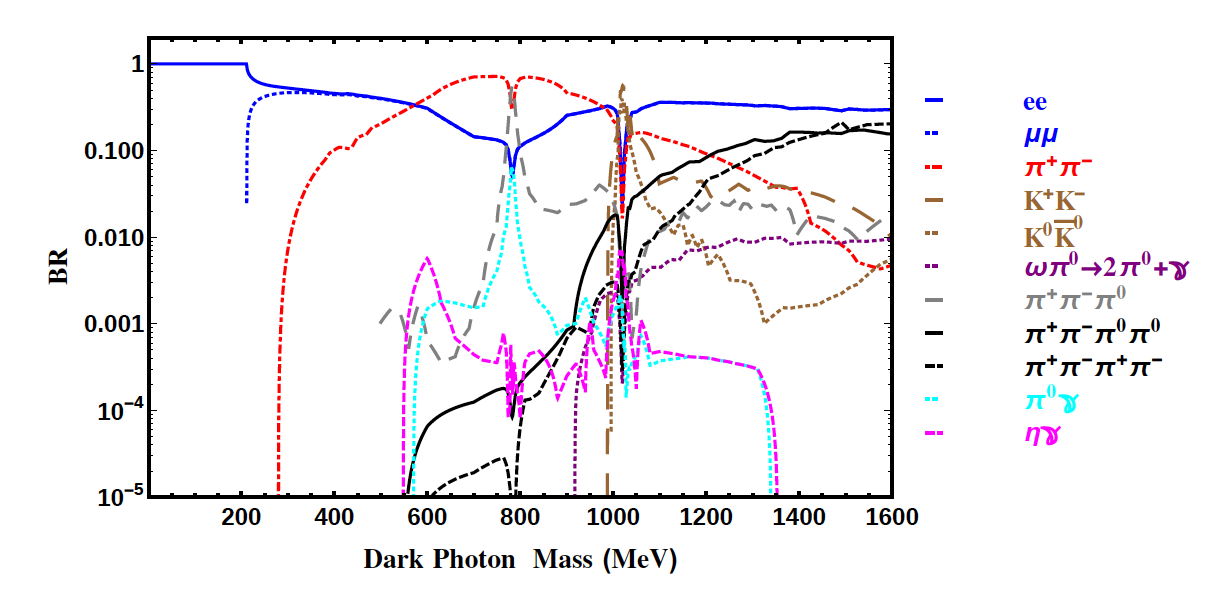
\includegraphics[width=0.9\textwidth]{pics/motivation/branchingRatio.png}
 	 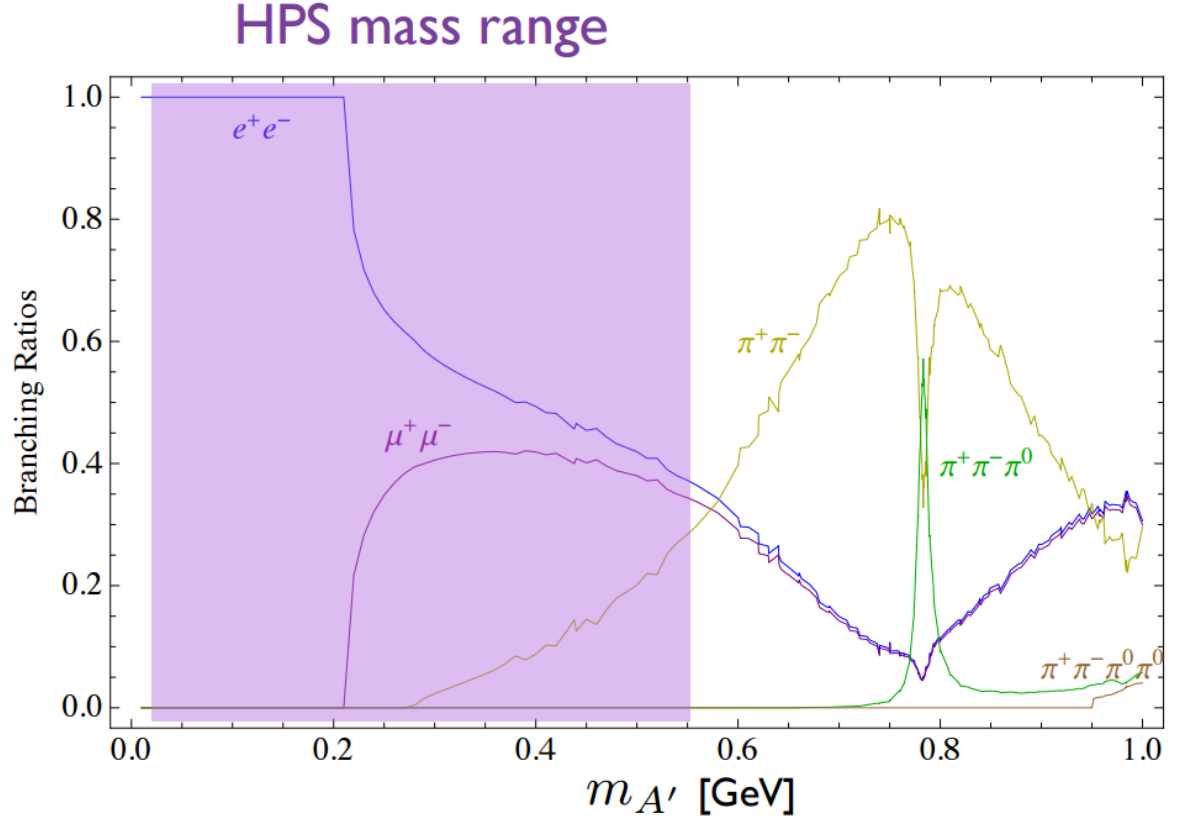
\includegraphics[width=0.5\textwidth]{pics/motivation/branchingLinear.png}	
  \caption[The branching fraction ratios for heavy photon decays]{The branching fraction ratios for heavy photons of various masses is shown~\cite{liu_signals_2015}. The top plot is shown for an extended mass range and log scale whereas the bottom plot shows a more limited mass range and linear scaling. The mass range that HPS is most sensitive to is highlighted in purple in the bottom plot.}
  \label{Figure:br}
\end{figure}

HPS searches for heavy photons of masses 20 to 100~MeV/c$^2$. As shown in Figure~\ref{Figure:br}, at heavy photon masses above 200~MeV/c$^2$, the branching ratio for decays to $e^+e^-$ decreases sharply and decays to $\mu^+\mu^-$ becomes significant. \\
\indent Assuming that the heavy photon only decays to SM final states, the proper lifetime of the $A^{\prime}$ neglecting phase space corrections is described by   

\begin{equation}
	\label{eq:propLife}
	\begin{split}
	c\tau &= \dfrac{1}{\Gamma}\simeq \dfrac{3}{N_{eff}m_{A^{\prime}}\alpha\epsilon^2}\\
	&\simeq \dfrac{0.8\textrm{ cm}}{N_{eff}}\Big({\dfrac{10^{-4}}{\epsilon}}\Big)^2\Big(\dfrac{100\textrm{ MeV}}{m_{A^{\prime}}}\Big)
	\end{split}
\end{equation}
where $N_{eff}$ is the number of available decay states ($=1$ at $m_{A^{\prime}}<2m_{\mu}$)~\cite{bjorken_new_2009}. The lifetime is inversely proportional to the coupling $\epsilon^2$. For small couplings, the heavy photon will travel a measurable distance before decaying. The decay length is 

\begin{equation}
	\label{eq:decayL}
	\begin{split}
	l_0 &\equiv \gamma c \tau \\
	&\simeq \dfrac{0.8\textrm{ cm}}{N_{eff}}\Big(\dfrac{E_{beam}}{10\textrm{ GeV}}\Big)\Big({\dfrac{10^{-4}}{\epsilon}}\Big)^2\Big(\dfrac{100\textrm{ MeV}}{m_{A^{\prime}}}\Big)^2
	\end{split}
\end{equation}
where $E_{beam}$ is the incident electron energy. The rate of $A^{\prime}$ production is dependent on $\alpha^3\epsilon^2/m_{A^{\prime}}^2$ and is suppressed relative to ordinary bremsstrahlung by a factor of $\epsilon^2m_{e^-}^2/m_{A^{\prime}}^2$~\cite{bjorken_new_2009}. The ratio of the fully differential production cross sections for the heavy photon relative to the production of a virtual photon is:

\begin{equation}
	\label{eq:production}
	\dfrac{d\sigma(e^-Z\rightarrow e^-ZA^{\prime}\rightarrow e^-Zl^+l^-)}{d\sigma(e^-Z\rightarrow e^-Z\gamma^{\ast}\rightarrow e^-Zl^+l^-)} = \Big(\dfrac{3\pi\epsilon^2}{2N_{eff}\alpha}\Big) \Big(\dfrac{m_{A^{\prime}}}{\delta m_{A^{\prime}}}\Big)
\end{equation}
This ratio represents the maximum signal to background that can be achieved in an experiment. The heavy photon is produced at very forward, small angles and carries nearly all of the beam energy. \\

\subsection{Methods of production}
Heavy photons can be produced experimentally in fixed-target experiments and collider experiments. Fixed-target experiments are complementary to collider experiments in that they can generally access smaller coupling due to the high luminosity while collider experiments can probe higher heavy photon masses due to the higher center of mass energy attainable. In electron fixed-target experiments, the heavy photon is generated through a bremsstrahlung-like process and is detected from the final state particles. Proton fixed-target experiments look for the signal in the decay products of various mesons produced from the beam interaction with the target. Looking for heavy photons produced in meson decays such as Dalitz decays ($\pi^0, \eta, \eta^{\prime}\rightarrow \gamma A^{\prime}$), ($K\rightarrow\pi A^{\prime} $, $\phi\rightarrow\eta A^{\prime}$, and $D^{\ast}\rightarrow D^{0}A^{\prime}$) are another production mechanism that has been used at both colliders and fixed target-type experiments. Drell-Yan ($q\bar{q}\rightarrow A^{\prime}$) experiments are more common at proton fixed target and hadron collider experiments. Both $e^+e^-$ colliders and hadron colliders search for heavy photons in the decay channels shown in Figure~\ref{Figure:br} and are particularly well-suited to search for heavy photons that decay invisibly due to their ability to precisely reconstruct the initial state. 

\subsection{Methods of detection}

The strategies for searching for heavy photons are typically a bump hunt on the visible final state particles, a bump hunt in the missing mass spectrum (for invisible decays), or a detached vertex search for heavy photons with small couplings. \\
\indent Electron fixed-target experiments produce heavy photons through bremsstrahlung-like processes with the electron beam incident on a heavy target. Heavy photons are produced in a very forward direction requiring high resolution spectrometers or detectors close to the beam. Previous limits set by this type of experiment include the A1 experiment that uses the Microtron beam at Mainz and the A1 high resolution spectrometer to reconstruct the $e^+e^-$ pair~\cite{beranek_theoretical_2013}. The A1 experiment significantly ruled out parameter space where the heavy photon was a possible explanation to resolve the muon $g-2$ anomaly. The APEX experiment at Jefferson Lab Hall A produced electron bremsstrahlung and used the high resolution spectrometers to measure the $e^+e^-$ particles~\cite{abrahamyan_search_2011}. APEX performed a bump hunt on the final state particles in the mass range 65-600~MeV and will likely take data again in 2018. DarkLight is another Jefferson Lab experiment that places a windowless gas target in the Low Energy Recirculator Facility using a 100~MeV beam to search for heavy photons with low masses. DarkLight will perform a bump hunt search in the $e^+e^-$ mass spectrum and may have some ability to search for invisible decays by using a silicon layer to detect proton recoils~\cite{balewski_darklight_2014}.\\
\indent Proton fixed target experiments look for heavy photons in the decays of particles produced from beam interactions at the target. The NA48/2 experiment at the CERN SPS produced $K^{\pm}$ beams and searched for heavy photons from the $\pi^0$ decay produced from the in-flight decay of the $K^{\pm}$~\cite{Batley_2015lha}. SHiP is a future experiment at the CERN SPS that will use a 400~GeV proton beam to look in both Drell Yan and meson decays for heavy photons. SHiP will be sensitive to long decay lengths (on the order of 10s of meters) and will cover a wide mass range in visible decay states up to 10~GeV masses. SHiP is expected to run sometime after 2026~\cite{ship_collaboration_facility_2015}.\\
\indent Beam dump experiments look for heavy photons with long decay lengths. The beam dump experiments E141 and E137 at SLAC, E774 at Fermilab, and one at Orsay were originally run to look for MeV-mass axion-type particles from electron beam dumps~\cite{alexander_dark_2016}. The U70 beam dump looked for heavy photons downstream from a proton beam on a fixed target~\cite{Blumlein:2013cua}. SeaQuest at Fermilab looks for muon pairs produced downstream from the 120~GeV proton beam on a fixed target. It is speculated that by analyzing previous data taken (E906/SeaQuest), a 95$\%$ confidence limit on heavy photon masses in the range of 215-5600~MeV is possible. SeaQuest is currently establishing upgrades for improved future running~\cite{gardner_new_2016}.\\
\indent Collider experiments using $e^+e^-$ or $pp$ collisions complement the fixed-target experiments and are favored for looking for heavy photon invisible decays.  BaBar, an experiment at the Stanford Linear Accelerator (SLAC) $e^+e^-$ collider, set limits by searching for the $A^{\prime}$ in missing mass around the $\Upsilon(2S)$, $\Upsilon(3S)$, and $\Upsilon(4S)$ resonances~\cite{Lees_2014xha}. In the near future, LHCb at CERN is expected to look for heavy photons in the di-muon invariant mass spectrum from rare heavy quark decays produced from proton-proton collisions. LHCb will be sensitive to the heavy photons with both prompt and displaced vertices and is expected to run sometime after 2021~\cite{Ilten_2016tkc}. The limits established by existing searches can be seen in Figure~\ref{Figure:projectedReach}.

\section{Heavy Photon Search kinematics}
The HPS experiment sends an electron beam through a thin tungsten target and looks for radiated heavy photons in the reconstructed $e^+e^-$ mass spectrum. HPS looks for heavy photons in the range of 20 to 1000~MeV/c$^2$ and covers this territory with two searches on the same data set that probe different heavy photon coupling regimes. A bump hunt searches for the heavy photon signal as a resonance on a large background. The bump hunt looks for heavy photons with large couplings and decay at the target. The vertex search looks for heavy photons that have detached vertices, having a measurable lifetime and decaying downstream of the target. 

\subsection{Signal}

The heavy photon is generated from the electron beam interaction with a heavy target as shown in Figure~\ref{fig:apTree} where $Z$ is the atomic number corresponding to the target material.  

\begin{figure}[htb]
    \begin{center}
	\begin{fmffile}{apTree}
	\begin{fmfgraph*}(150,150)
	\fmfstraight
		\fmfleft{i1,i2,i3,i4}
		\fmfright{o1,o2,o3,o4}
		\fmflabel{$Z$}{i1}
		\fmflabel{$e^-$}{i2}
		\fmflabel{$e^-$}{o2}
		\fmflabel{$e^-$}{o3}
		\fmflabel{$e^+$}{o4}	
		\fmf{heavy}{i1,v1,o1}
		\fmffreeze
		\fmf{fermion}{i2,v2,v3,o2}				
		\fmffreeze	
		\fmf{fermion}{o4,v4,o3}
		\fmf{photon,tension=0,label=$\gamma$}{v1,v2}
		\fmf{photon,tension=2,label=$A^{\prime}$}{v3,v4}
	\end{fmfgraph*}
	\end{fmffile}
  	\end{center}
    	\caption[Heavy photon production in a fixed-target experiment]{The heavy photon is produced in a process analagous to bremsstrahlung on a heavy target of atomic number $Z$.}
   	 \label{fig:apTree}	
\end{figure}

Shown for the HPS experiment, the heavy photon decays to $e^+e^-$ pairs with a measurable mass and possible displaced vertex downstream from the target. The differential cross section for heavy photon production is 

\begin{equation}
	\label{eq:apDiffCS}
	\dfrac{d\sigma}{dxd\cos\theta_{A^{\prime}}} \approx \dfrac{8Z^2\alpha^3\epsilon^2E_0^2x}{U(x,\theta_{A^{\prime}})^2}\log\Big( (1-x+\dfrac{x^2}{2})-\dfrac{x(1-x)m_{A^{\prime}}^2E_0^2x\theta_{A^{\prime}}^2}{U(x,\theta_{A^{\prime}})^2}\Big)
\end{equation}
where $Z$ is the atomic number of the target material, $\alpha$ is the usual fine structure constant, $\theta_{A^{\prime}}$ is the lab frame angle of the outgoing heavy photon, $E_0$ is the electron incident energy, $m_{A^{\prime}}$ is the heavy photon mass, and the fraction of incident beam energy carried by the the heavy photon is $x\equiv E_{A^{\prime}}/E_0$~\cite{bjorken_new_2009}. The virtuality of the intermediate electron is described by

\begin{equation}
	\label{eq:virtuality}
	U(x,\theta_{A^{\prime}}) = E_0^2x\theta_{A^{\prime}}^2+m_{A^{\prime}}^2\dfrac{1-x}{x}+m_e^2x 
\end{equation}
where $m_e$ is the mass of the electron. The cross section is further simplified for $m_e\ll m_{A^{\prime}}\ll E_0$ and $x\theta_{A^{\prime}}^2\ll 1$. Integrating Equation~\eqref{eq:apDiffCS} over the angle, the cross section is

\begin{equation}
	\label{eq:csFinal}
	\dfrac{d\sigma}{dx} \approx \dfrac{8Z^2\alpha^3\epsilon^2x}{m_{A^{\prime}}^2}\Big(1+\dfrac{x^2}{3(1-x)}\Big)
\end{equation}
The total heavy photon production rate is proportional to $\alpha^3\epsilon^2/m_{A^{\prime}}^2$ and is suppressed relative to photon bremsstrahlung by $\epsilon^2m_e^2/m_{A^{\prime}}^2$.The singularity is regulated by the mass of the electron and cutoff for values where $1-x$ exceeds $m_e^2/m_{A^{\prime}}^2$ or $m_{A^{\prime}}^2/E_0^2$. The heavy photon carries nearly the entire beam energy such that the median value of $1-x\sim\textrm{max}\Big(\dfrac{m_e}{m_{A^{\prime}}}, \dfrac{m_{A^{\prime}}}{E_0}\Big)$. The heavy photon is emitted predominately at small angles with a cutoff at $\dfrac{m_{A^{\prime}}^{3/2}}{E_0^{3/2}}$ such that the angular emission falls off as $1/\theta_{A^{\prime}}^4$.\\
 \indent The heavy photon is characterized by its mass (as reconstructed from the decay to $e^+e^-$) and decay length. Depending on the coupling strength $\epsilon$, the vertex may be reconstructed from a prompt decay at the target or a measurable decay downstream.  

\subsection{Backgrounds}

The primary backgrounds in this experiment include trident events and wide angle bremsstrahlung (WAB). The tridents have the same three particle final state $e^-e^-e^+$ and are broadly categorized into radiative and Bethe-Heitler diagrams~\cite{bjorken_new_2009}. The trident events were the primary source of background considered prior to running the experiment. It was later found that WAB events contributed to the background with an $e^-\gamma$ final state where the photon then produced an $e^+e^-$. In many cases, the event was triggered by the initial electron and pair-produced positron. 

\begin{figure}[htb]
    \begin{center}
	\begin{fmffile}{radTree}
	\begin{fmfgraph*}(150,150)
	\fmfstraight
		\fmfleft{i1,i2,i3,i4}
		\fmfright{o1,o2,o3,o4}
		\fmflabel{$Z$}{i1}
		\fmflabel{$e^-$}{i2}
		\fmflabel{$e^-$}{o2}
		\fmflabel{$e^-$}{o3}
		\fmflabel{$e^+$}{o4}	
		\fmf{heavy}{i1,v1,o1}
		\fmffreeze
		\fmf{fermion}{i2,v2,v3,o2}				
		\fmffreeze	
		\fmf{fermion}{o4,v4,o3}
		\fmf{photon,tension=2,label=$\gamma$}{v1,v2}
		\fmf{photon,tension=2,label=$\gamma$}{v3,v4}
	\end{fmfgraph*}
	\end{fmffile}
  	\end{center}
    	\caption[Radiative background]{Radiative trident background process: The photon is radiated from the electron incident on a heavy target of atomic number $Z$ and produces and $e^+e^-$ pair. The radiatives have the same kinematics as the heavy photon and comprise the primary background in the bump hunt analysis where all decays are prompt. }
   	 \label{fig:radTree}	
\end{figure}

The radiative background is irreducible and comprises the smooth background upon which the bump hunt search for the heavy photon signal is conducted. The Bethe-Heitler tridents also contribute significantly to the background although they are peaked at lower $e^+e^-$ total energy. The Bethe-Heitler contribution is shown in Figure~\ref{fig:bhTree}. The radiative and Bethe-Heitler diagrams also interfere, although, this generally only contributes at lower $e^+e^-$ total energy. 

\begin{figure}[htb]
    \begin{center}
	\begin{fmffile}{bhTree}
	\begin{fmfgraph*}(150,150)
	\fmfstraight
		\fmfleft{i1,i2,i3,i4}
		\fmfright{o1,o2,o3,o4}
		\fmflabel{$Z$}{i1}
		\fmflabel{$e^-$}{i4}
		\fmflabel{$e^-$}{o2}
		\fmflabel{$e^+$}{o3}
		\fmflabel{$e^-$}{o4}	
		\fmf{heavy}{i1,v1,o1}
		\fmffreeze
		\fmf{fermion}{i4,v4,o4}				
		\fmffreeze	
		\fmf{photon,tension=1,label=$\gamma$}{v1,v2}
		\fmf{photon,tension=1,label=$\gamma$}{v3,v4}
		\fmf{fermion}{o3,v3,v2,o2}
	\end{fmfgraph*}
	\end{fmffile}
  	\end{center}
    	\caption[Bethe-Heitler background]{Bethe-Heitler trident background process: The photon produced from electron interaction at a target of atomic number $Z$ produces an $e^+e^-$ pair that often have a total energy much less than the initial beam energy. The recoil electron and the Bethe-Heitler positron can also be detected.}
   	 \label{fig:bhTree}	
\end{figure}
%%%%%%%%%%%%%%%%%%%%%%%%%%%%%%%%%%%%%%%%%
\chapter{Heavy Photon Search Experiment}
%The HPS experiment used a Silicon Vertex Tracker (SVT) and an electromagnetic calorimeter (ECal). The SVT, located inside of a dipole magnet, measures particle momenta and the interaction vertex position of the $e^+e^-$ pairs. The ECal triggers the readout of physics events and measures particle energy and time. \par
The HPS experiment is located in the downstream alcove of Hall B at Jefferson Lab. The Continuous Electron Beam Accelerator Facility (CEBAF) produces an electron beam which passes through Hall B to the alcove where the beam interacts with the HPS target housed inside the pair spectrometer magnet with the SVT. This interaction yields particle pairs and beam scattered electrons which pass through the six layers of the SVT before depositing their energy in the ECal for event readout.

\section{Continuous Electron Beam Accelerator Facility}

The CEBAF accelerator at Jefferson Lab generates the electron beam used in the HPS experiment. CEBAF can deliver continuous electron beams to multiple experimental halls simultaneously. The CEBAF accelerator is a recirculating linac in the shape of a racetrack through which electron beam bunches can pass multiple times, boosted in energy with each pass, before being delivered to a specific hall. 

\begin{figure}[htb]
  \centering
      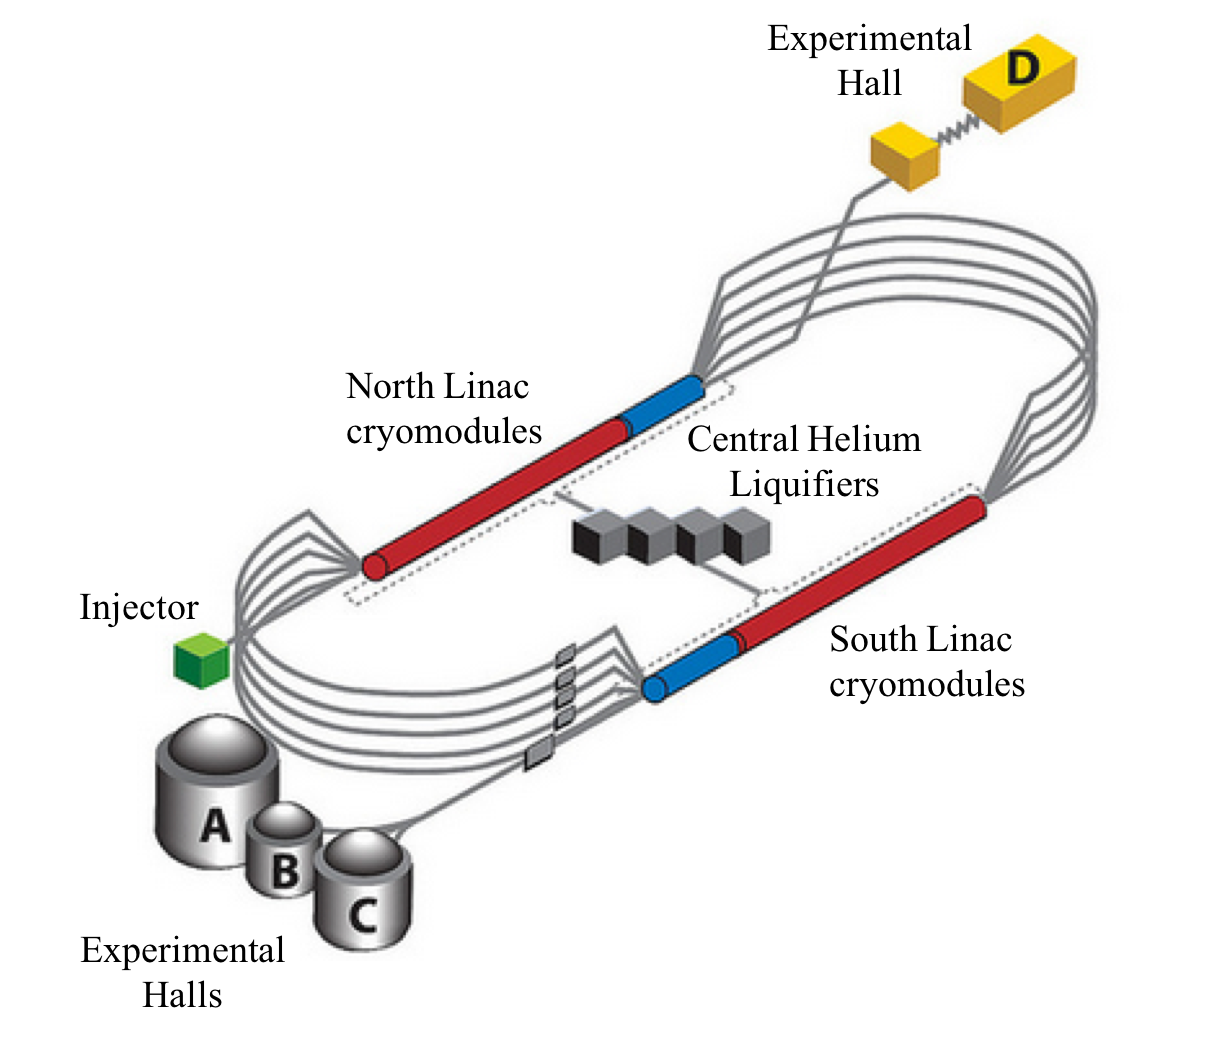
\includegraphics[width=0.75\textwidth]{pics/experiment/cebafLabel.png}
  \caption[CEBAF accelerator]{A drawing of the CEBAF accelerator. The electron beam is produced at the injector and can circulate through up to five passes around the race track design of the accelerator. There are four experimental halls that can receive beam and run experiments, simultaneously: A, B, C, and D. CEBAF was upgraded prior to the HPS experiment to include additional cryomodules, a second Central Helium Liquifier (CHL), and a fifth pass in order to produce higher energy.}
  \label{Figure:cebaf}
\end{figure}

CEBAF can provide continuous electron beams with energies up to 12~GeV and intensities up to approximately 100~$\mu$A to each of the four experimental halls. CEBAF was upgraded from producing 1.1~GeV per pass to 2.2~GeV per pass in 2014. 
%The injector energy is 100~MeV, designed for a maximum of five passes (upgraded from four passes) with %an energy per pass of 2.2~GeV (upgraded from 1.1~GeV). These upgrades double the maximum energy %output of the accelerator. While the accelerator frequency operates at 1500~MHz, a new 750~MHz RF %separator was installed in order to provide beam to all four halls simultaneously. With these upgrades, the %halls can receive the beam at 250 or 500~MHz and operate at different energies \cite{Kazimi_2013}. 

HPS was the first experiment to run in Hall B after the accelerator was upgraded. After a problem occurred in one CHL during the Engineering Run in the spring of 2015, HPS obtained dedicated beam time as one of the few experiments that could continue to take physics data with the accelerator operating at a single pass using the remaining CHL. The resulting energy for the Engineering Run, 1.05~GeV, would have been impossible to obtain with the simultaneous running of other experiments requiring 2.2~GeV per pass.  

\section{Beamline}
The HPS experiment is installed in the downstream alcove of experimental Hall B at Jefferson Lab as shown in Figure~\ref{Figure:hallB}~\cite{beamline_nim_2017}. Due to the construction of the CLAS12 detector in Hall B as part of the 12~GeV upgrade, HPS running was planned for nights and weekends when running beam would not interfere with CLAS12 construction. After the partial failure of the CHL, HPS received dedicated, continuous running during May of 2015 in support of the Engineering Run. 

\begin{figure}[htb]
  \centering
      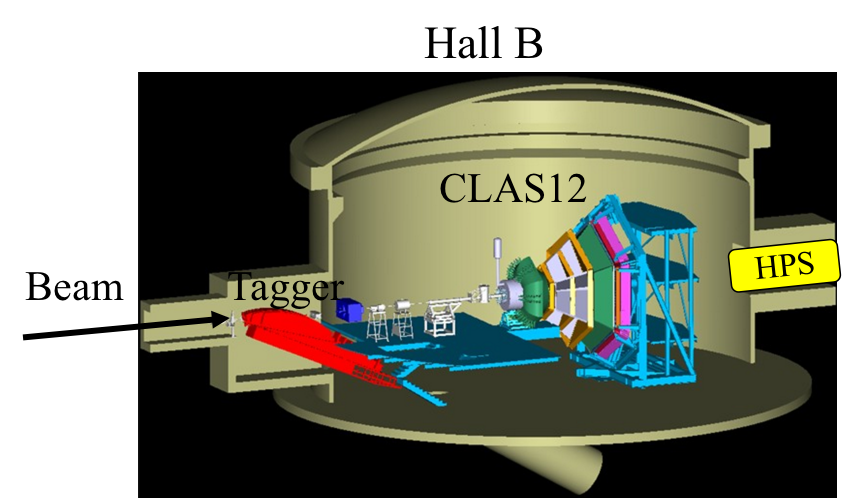
\includegraphics[width=0.6\textwidth]{pics/experiment/hallB.png}
  \caption[HPS location in Hall B]{The HPS experiment is in the downstream alcove of Hall B and ran while not interfering with CLAS12 construction.}
  \label{Figure:hallB}
\end{figure}

\begin{figure}[htb]
  \centering
      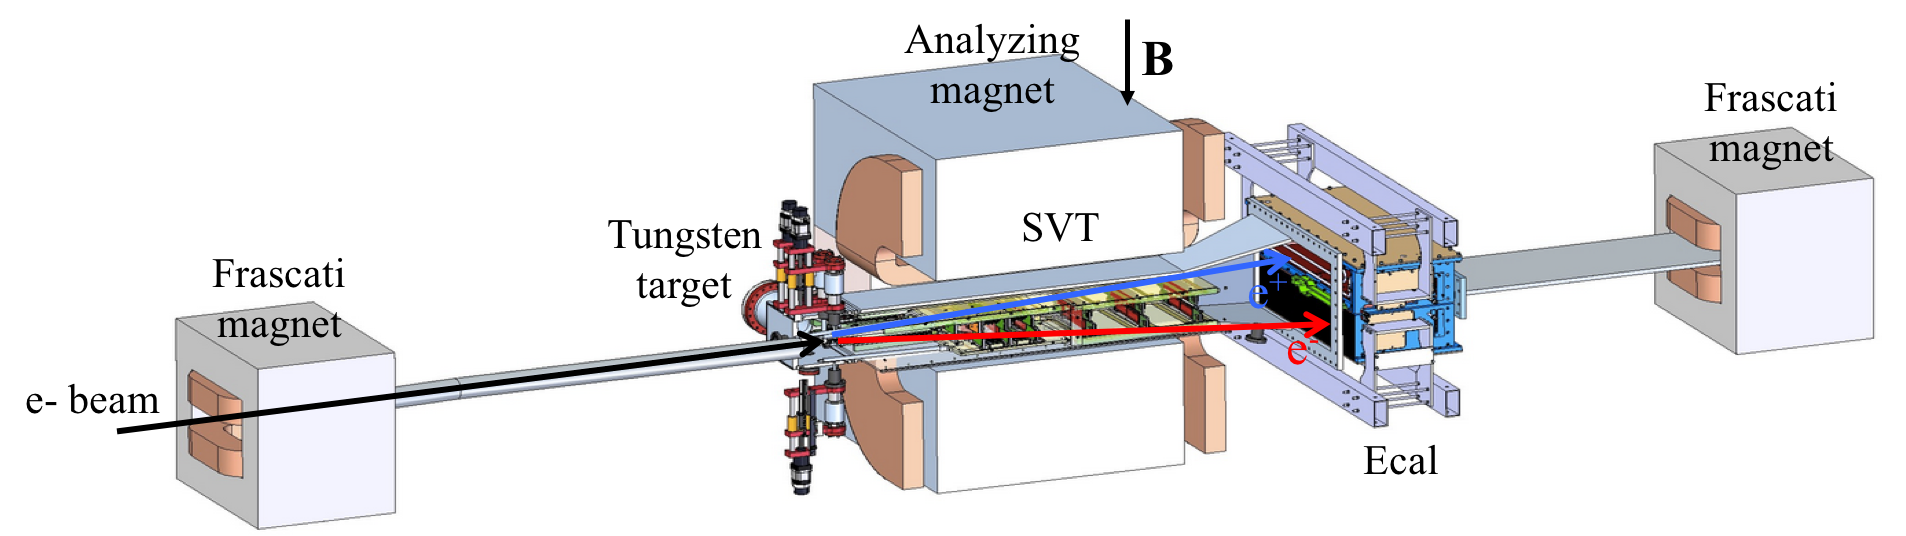
\includegraphics[width=1.0\textwidth]{pics/experiment/hpsBeamline.png}
  \caption[HPS beamline]{A drawing of the HPS experiment. After the electron beam passes through Hall B and into the alcove, the beam enters the first Frascati magnet. The electron beam hits the tungsten target, located in the Pair Spectrometer magnet, at an angle of approximately 30.5~mrad. Particles created from the interaction of the beam at the target pass through the six tracking layers of the SVT before depositing their energy into the ECal.}
  \label{Figure:hpsBeamline}
\end{figure}

\begin{figure}[htb]
  \centering
      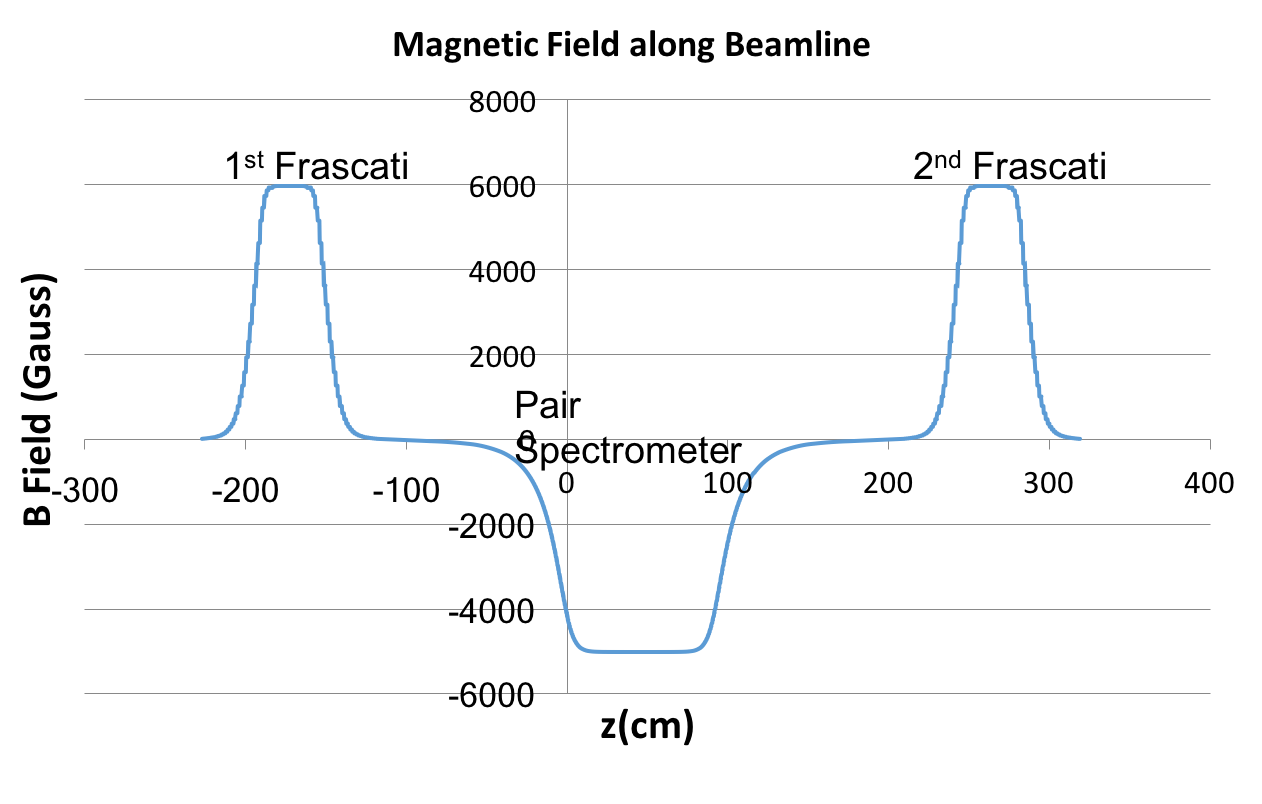
\includegraphics[width=1.0\textwidth]{pics/experiment/bfield.png}
  \caption[HPS magnetic fields]{The dipole magnetic field values for 2.2~GeV running where $z$ is the distance along the beamline from the target.}
  \label{Figure:bField}
\end{figure}

\begin{figure}[htb]
  \centering
      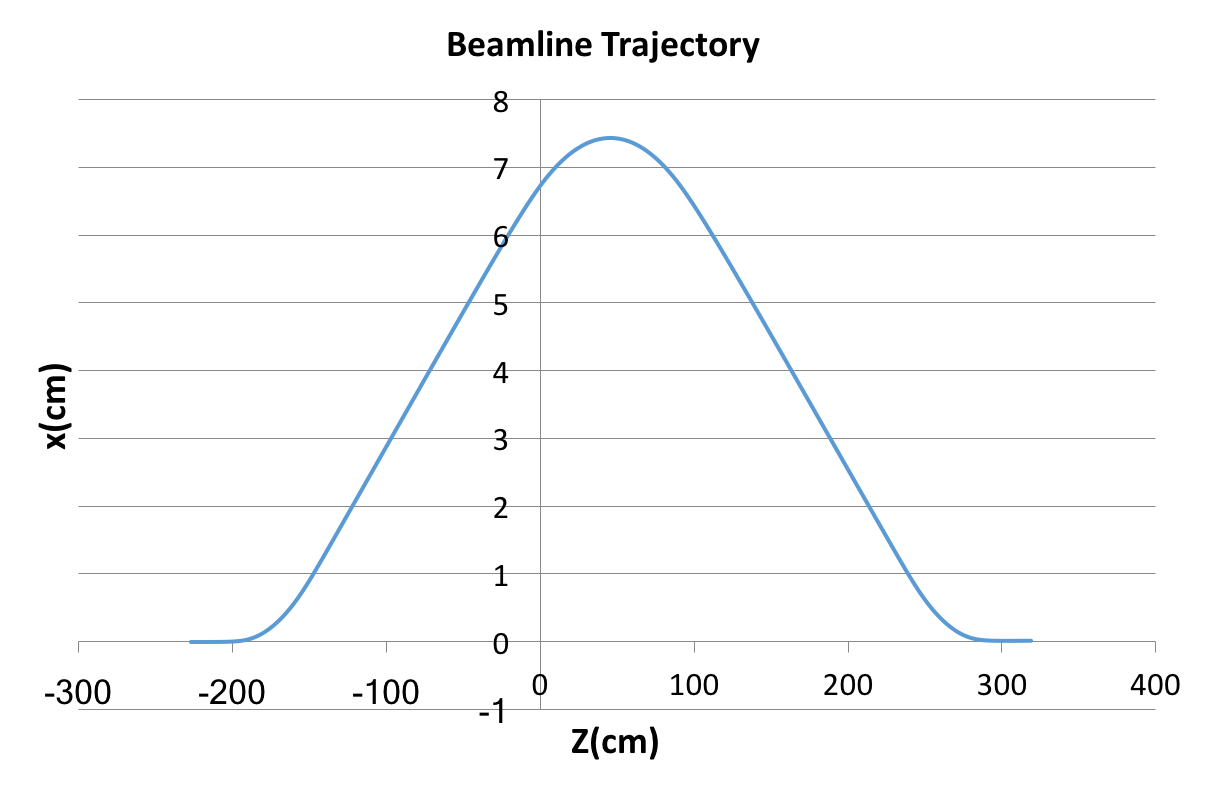
\includegraphics[width=1.0\textwidth]{pics/experiment/feetrajectory.png}
  \caption[Charged particle trajectory in HPS beamline]{The horizontal trajectory of a 2.2~GeV electron through the three dipole chicane along the beamline where $z$ is the distance along the beamline and $x$ is transverse to $z$. The target position is at $z=0$.}
  \label{Figure:trajectory}
\end{figure}

\begin{figure}[htb]
  \centering
      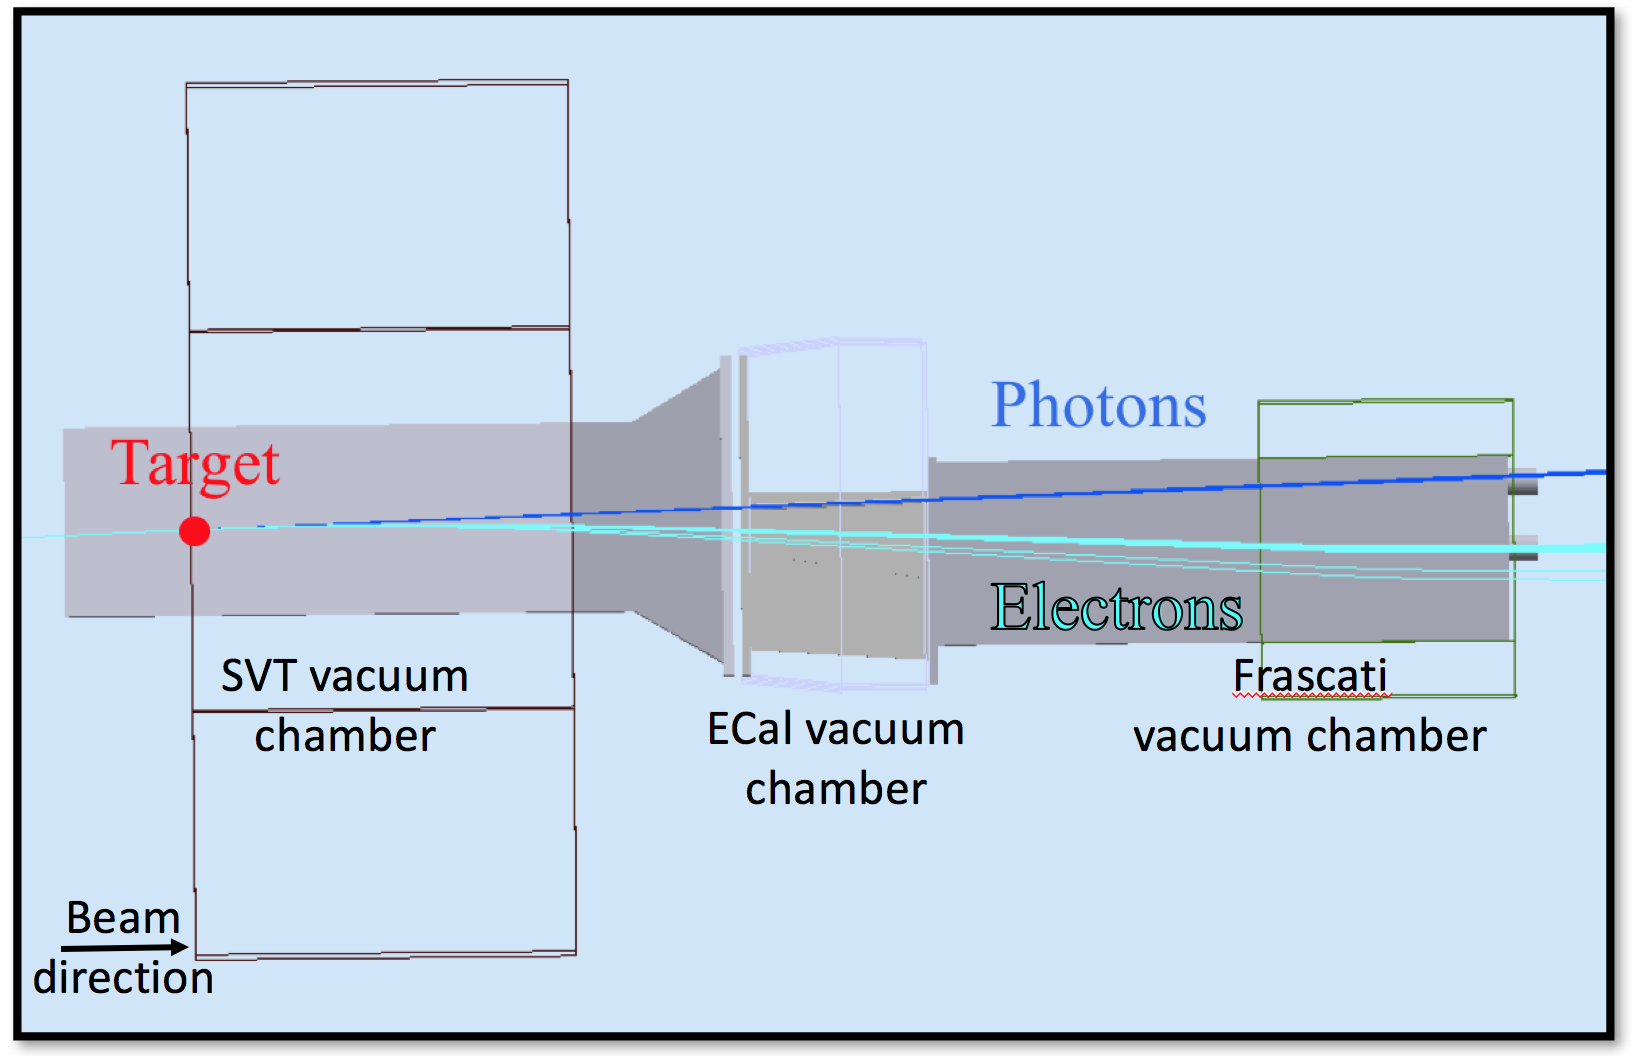
\includegraphics[width=0.8\textwidth]{pics/experiment/hpsbeam_v2.png}
  \caption[HPS beamline simulation in GEMC]{A bird's eye view of the HPS beam line shows the straight line trajectory of the photons from the HPS target through the SVT, ECal, and last vacuum chamber. The trajectory of the electrons in the magnetic field can be seen as passing through the cut outs in the vacuum chambers in order to pass through to the beam dump. The photons also have a clear, straight-line trajectory through the HPS vacuum chambers.}
  \label{Figure:gemc}
\end{figure}

%\begin{figure}[htb]
%  \centering
%      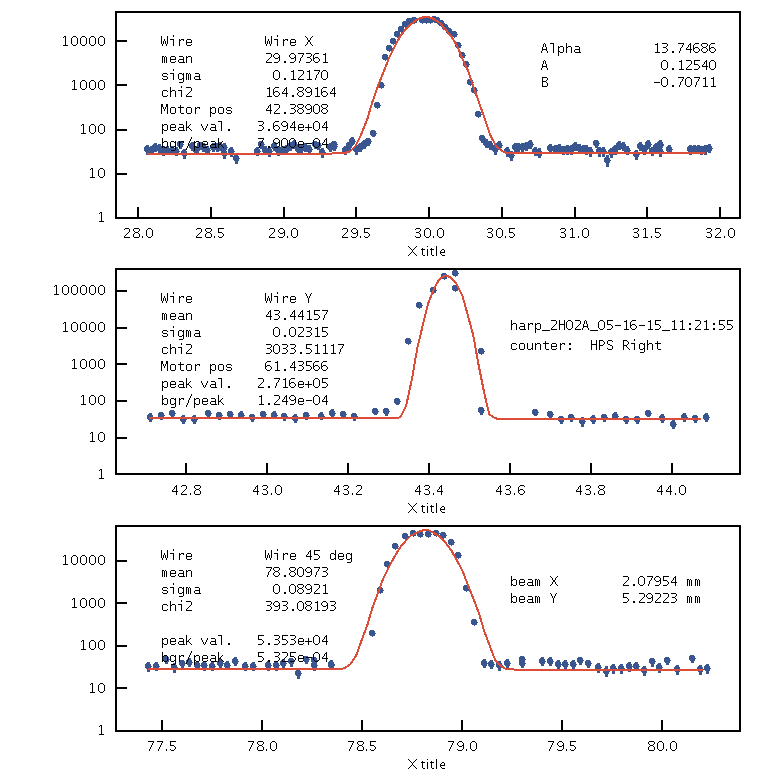
\includegraphics[width=0.75\textwidth]{pics/experiment/harpScan.png}
%  \caption[Beam profile from harp scan during 2015 run]{Harp scan showing the beam profile during May 2015 running. This particular harp scan is in the Hall B logbook, entry 3341231. The beam line profile in this scan is 122$\mu$m wide in $x$ by 23$\mu$m in $y$.}
%  \label{Figure:harpScan}
%\end{figure}

\begin{figure}[hbt]
%\begin{center}
\begin{minipage}{0.65\textwidth}
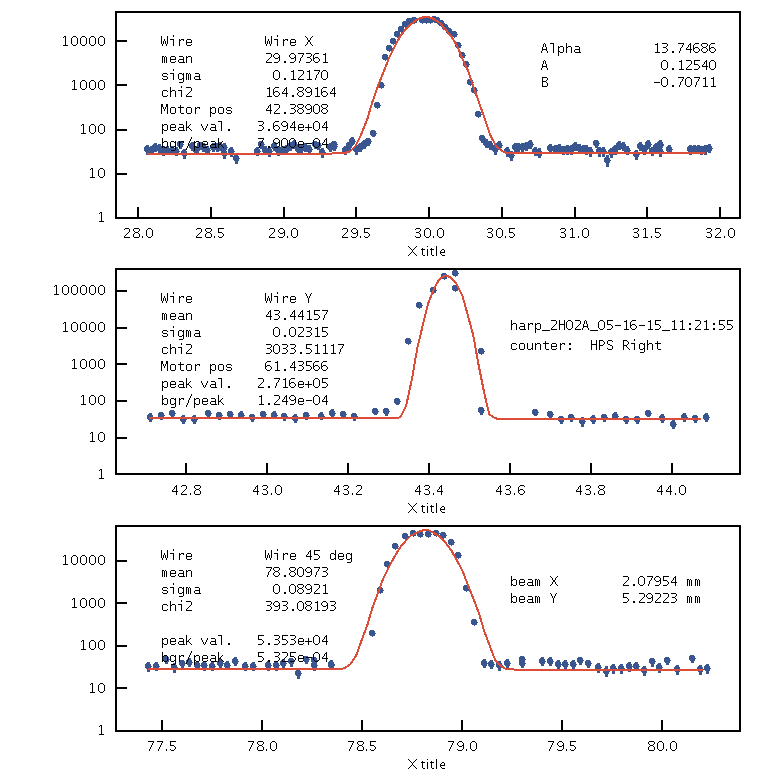
\includegraphics[width=\textwidth]{pics/experiment/harpScan.png}
%\end{center}
\end{minipage}\hfill\begin{minipage}{0.32\textwidth}
\caption[Beam profile from harp scan during 2015 run]{ \label{fig:harpScan} \baselineskip 11pt
Harp scan showing the beam profile during May 2015 running. This particular harp scan is in the Hall B logbook, entry 3341231. The beam line profile in this scan is 122$\mu$m wide in $x$ by 23$\mu$m in $y$.}
\end{minipage}
\end{figure}


The tagger magnet as depicted in Figure~\ref{Figure:hallB} was used for initial beam tuning from the accelerator before sending the beam through to the HPS detectors. By energizing the tagger magnet, the electron beam was visible at the tagger dump viewer and could be aligned at the center of the viewer. Before sending the beam to HPS, harp scans were performed to measure the position and width of the beam spot~\cite{beamline_nim_2017}. Once the harp scans showed the beam to be of an acceptable size and position upstream of HPS, the tagger magnet was de-gaussed for HPS running. Without the tagger magnet on, the electron beam passes through the hall to the HPS setup as shown in Figure~\ref{Figure:hpsBeamline}. \\
\indent The HPS setup consists of a three-dipole chicane with magnetic fields in the vertical direction. The target and the SVT are housed in the central magnet known as the pair spectrometer, or analyzing magnet. The pair spectrometer has a pole length of 91.44~cm and width of 45.72~cm. For 2.2~GeV electrons, the central magnetic field of the pair spectrometer magnet is 0.5~T~\cite{beamline_nim_2017}. For other beam energies, the analyzing magnet magnetic field is scaled accordingly. In the Engineering Run in May 2015, with a beam energy of 1.056~GeV, the pair spectrometer had a central field value of 0.24~T. The Frascati magnets, one on each side of the analyzing magnet, have magnetic fields opposite to that of the analyzing magnet such that the integrated field value over the length of the pole value of each Frascati is half of the integrated field value of the analyzing magnet. This ensures that the beam will end at the same location whether the chicane is energized or not and that the trajectory of beam energy electrons in the magnetic field is consistent across different beam energies. The magnetic field of the HPS beam line in the chicane is shown in Figure~\ref{Figure:bField}.\\
\indent The magnetic fields of the magnets were carefully measured and mapped. The trajectory of particles was studied using these magnetic field maps that included fringe field effects. The position of the pair spectrometer magnet with respect to the Frascati magnets was optimized from these field mappings. The horizontal trajectory of a beam energy electron is shown in Figure~\ref{Figure:trajectory}.\\
\indent In Figure~\ref{Figure:trajectory}, the target position is where at $z=0$. The entry angle of the beam at the target was determined to be approximately 30.5~mrad. At 70~cm from the target, the pair spectrometer magnet and vacuum chamber are centered on the position of the photon trajectory from the target such that the photons pass unobstructed through all subsequent vacuum chambers. The pair spectrometer magnet was placed 8.87~cm beam left, thus placing the HPS target position 2.14~cm to the right of the magnet center line. By modeling the vacuum chambers and magnetic fields in the GEant4 Monte Carlo (GEMC) framework, the particle trajectories through the HPS beam line can be observed as in Figure~\ref{Figure:gemc}.\\
\indent As shown in Figure~\ref{Figure:gemc}, the beam energy electrons pass through the exit hole of the last vacuum chamber (contained in the second Frascati dipole) and continue traveling to the Faraday cup where the beam charge can be measured. The beam line was modeled in GEMC and, in real running, utilized a multitude of monitors to ensure clear passage of the beam.\\
\indent The passage of the beam through the HPS beam line was monitored using beam position monitors (BPMs), wire scans with halo counters, beam viewers, and a Faraday cup. The three upstream nA BPMs gave continuous beam current and position readings. These BPMs can indicate that the beam is scraping the beam pipe when the current readings fluctuate and differ with respect to each other. The current readings from the BPMs were compared to the current reading at the Faraday Cup (located downstream of the HPS beam line at the dump). When the beam current is at 50~nA or below, the reading at the Faraday Cup current is roughly the same as the current read out by the upstream BPMs and indicates no beam scraping in the beam pipe. When operating at currents above 50~nA, it was standard to insert a beam blocker in front of the Faraday Cup in order to protect it. The beam stopper would then create an offset in the Faraday Cup current readout and the actual beam current. Additionally, a fluorescent viewer screen at the Faraday Cup was used to show the beam position.  A video camera streaming a view of the screen was used for remotely observing the relative beam position on the screen. \\ 
\indent Harp scans measured the current and position of the beam through interaction with the beam (as compared to the passive, continuous readout employed through the BPMs). A harp scan moves wires through the beam vertically, horizontally, and diagonally while  downstream halo counters measure the scattered beam electron spray. The halo counters are photomultiplier tubes (PMT) strapped around the beam pipe line. The intensity of the electron spray detected by the PMTs is proportional to the beam charge interacting with the wire. A typical harp scan from the Engineering Run is shown in Figure~\ref{fig:harpScan}.\\
\indent The beam profile is narrower in $y$ (vertically) than in $x$ (horizontally). The proposed beam profile for the HPS experiment was 50~$\mu$m in $y$ and 300~$\mu$m in $x$ in order to prevent overheating at the target and allow for precise vertex reconstruction. While overheating was not a limiting factor in the experiment, most of the 2015 running had a beam profile of no larger than 50~$\mu$m in $y$ and 150~$\mu$m in $x$. 

\subsection{Beam line protection}
The SVT is ideally as close to the beam as possible in order to maximize acceptance for heavy photons. The nominal SVT position has the first layer of the SVT at $\pm0.5$~mm from the active beam. Passive and active measures were employed during experimental running to prevent damage to the silicon if the beam position or quality changes during running. The collimator is a 1~cm thick tungsten plate placed upstream of the SVT with a slit through which the beam can pass. A collimator prevents direct damage to the silicon should the beam move vertically from its nominal position by diffusing the beam. For the Engineering Run, the 4~mm slit width was used. \\
\indent The active beam line protection element is the Fast Shut Down (FSD) system.The FSD, when triggered, can shut off the electron beam in 1~ms. HPS used the halo counters closest to the HPS experiment to trigger the FSD when the beam shifted or the quality significantly deteriorated. When the beam shifted vertically, it would first hit the inactive region of the SVT silicon sensors and scatter, increasing the rates in the halo counters. When the rates surpassed a pre-determined threshold, the FSD was tripped. If the beam hit the collimator, this also increased the rates in the halo counters and tripped the FSD. 

\subsection{Target}

The primary HPS target is a thin tungsten foil that is mounted on a support frame that can be fully retracted from the beam when not in use. For 1.1~GeV and 2.2~GeV running, the design thickness of the target tungsten foil is 0.125$\%$ radiation lengths (approximately 4~$\mu$m). The measured thickness of the actual target was 0.116$\%$. There is also a tungsten target of 0.25$\%$ radiation lengths for future running at 4.4~GeV and 6.6~GeV. The target support frame inserts the foil target from above the beam using a stepping motor linear actuator. The bottom of the target foil is frame-less so that the target can be inserted into the active beam without interruption.   

\section{Silicon Vertex Tracker}
\begin{figure}[htb]
  \centering
      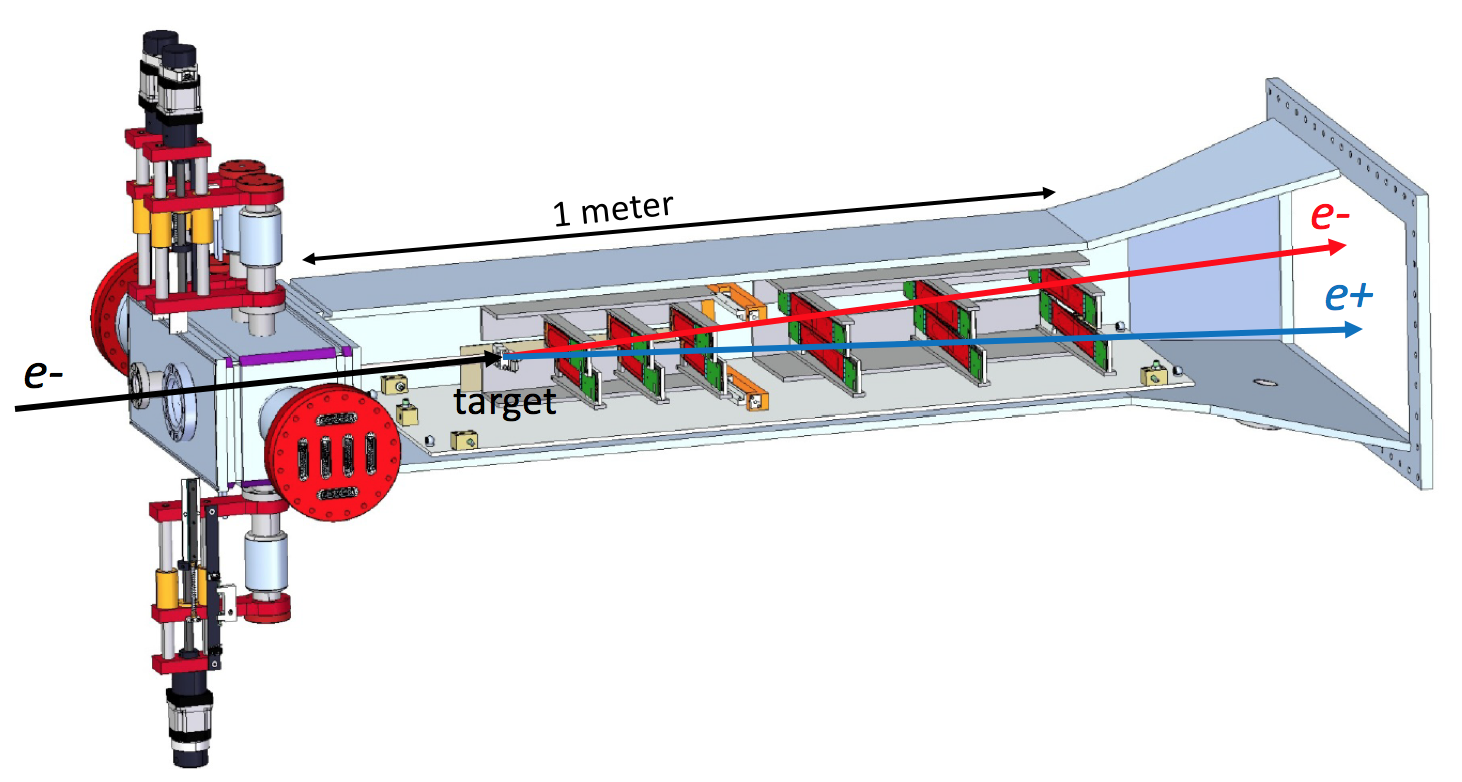
\includegraphics[width=1.0\textwidth]{pics/experiment/svt.png}
  \caption[Rendering of the HPS SVT]{A rendering of the HPS SVT. The beam enters from the left through the vacuum box. The silicon sensors are shown in red, and the hybrid readout boards are shown in green.}
  \label{Figure:svt}
\end{figure}

\begin{figure}[h]
  \centering
      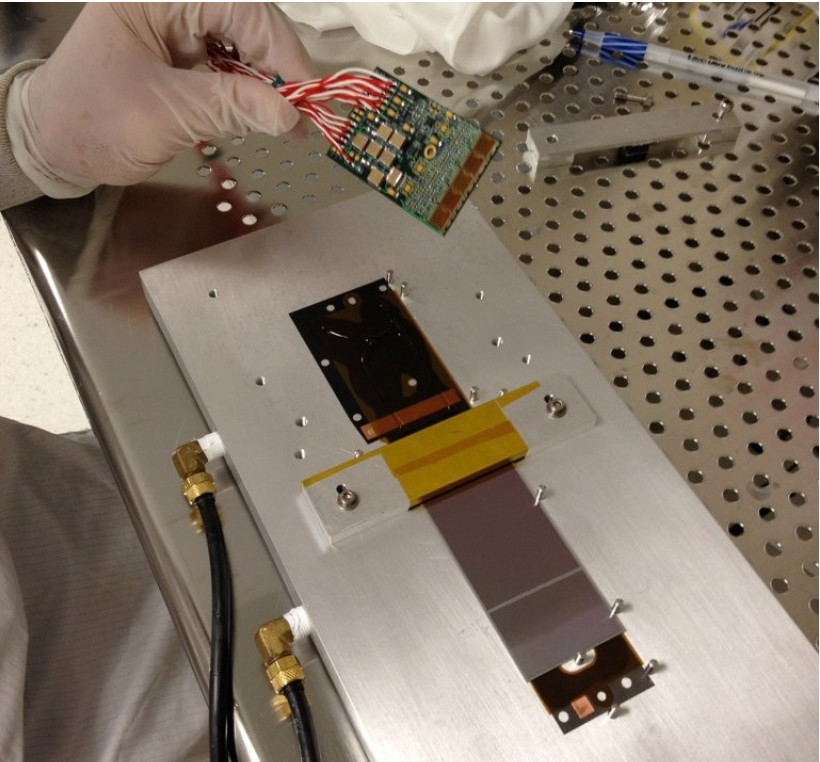
\includegraphics[width=0.5\textwidth]{pics/experiment/svtSensorAssembly.png}
  \caption[Assembly of a half module of the SVT ]{A half module is being assembled for Layers 1-3 of the SVT. A readout hybrid with the APV25 chips is being attached to the frame along the silicon sensor.~\cite{collaboration_heavy_2013}}
  \label{Figure:svtAssembly}
\end{figure}

The Silicon Vertex Tracker (SVT) measures particle momentum and trajectories through a magnetic field in order to reconstruct the invariant mass and the vertex position of the $e^+e^-$ pair. The SVT is composed of six layers of 0.7$\%$ radiation length-thick silicon placed downstream of the target and housed in a vacuum chamber within the analyzing magnet. The SVT is separated into top and bottom halves that can be positioned vertically above and below the beam. Nominally, the SVT operates with a 15~mrad opening angle such that the first layer of the SVT is at $\pm$0.5~mm from the active beam. A drawing of the SVT is shown in Figure~\ref{Figure:svt}.

The SVT is located in a magnetic field such that particles are bent horizontally (field points downward). Each of the six layers is composed of two silicon strip detectors capable of measuring a hit position in one dimension. By setting the strips at a stereo angle with respect to one another, each layer of the SVT is capable of three-dimensional hit reconstruction. The first three layers of the SVT are one silicon strip sensor-wide and have a stereo angle of 100~mrad between the strips. The last three layers of the SVT are two strip sensors-wide in order to better match the Ecal acceptance. The stereo angle between the sensors in layers four through six is 50~mrad. The axial sensors are oriented horizonally whereas the stereo sensors are angled with the lower end closer to the beam plane on the positron side (beam left) where the background is less intense. The different stereo angles are used to eliminate ghost hits that can generate ghost tracks. The first five layers of the SVT cover the Ecal acceptance while the sixth layer has a slightly reduced acceptance but can be used to improve track reconstruction. The full track reconstruction only requires five hits per track in order to pick up tracks that may be missing hits due to an inefficiency. \\
\indent The hybrid readout boards on each sensor house the APV25 readout chips that connect the sensor to the data acquisition (DAQ) system. The power to the APV25 chips is supplied through the hybrid, and the temperature of the strip is actively monitored at the hybrid. The heat generated by the operating hybrid  flows through the aluminum support structure. As the sensors are cooled for operation, the support structure and sensor contract at slightly different rates. In order to maintain the sensor at a constant tension, one end of the sensor is attached to a spring pivot. The assembly of a silicon sensor is shown in Figure~\ref{Figure:svtAssembly}.

The APV25 samples the signals on the strips every 24~ns and stores the results in a pipeline. Once a trigger is received, the pipelines are read out. The readout yields six samples at 24~ns intervals that can be fit to reconstruct the waveform. A 4-pole functional fit was used to extract the time and amplitude of the corresponding hit. A latency time that is configured in the SVT DAQ is used to correctly determine which channel pipelines are read out that correspond to the trigger. The latency time is approximately equal to the time delay of the trigger. Some early data in the Engineering Run was lost due to incorrect latency timing. 


\section{Electromagnetic Calorimeter}
The ECal was used to trigger events and measure particle energy and timing. The ECal is a homogeneous calorimeter comprised of 442 trapezoidal PbWO$_4$ scintillating crystals, each read out by a large area avalanche photodiode (APD) attached to the back of each crystal~\cite{Balossino201789}. The crystals are re-purposed from the former CLAS IC detector and have been upgraded with larger avalanche photodiodes. Each crystal is trapezoidal in shape and 16~cm long with the front and back faces 1.3$\times$1.3~mm$^2$ and 1.6$\times$1.6~mm$^2$, respectively. The calorimeter layout is shown in Figure~\ref{Figure:ecalface}. 

\begin{figure}[h]
  \centering
      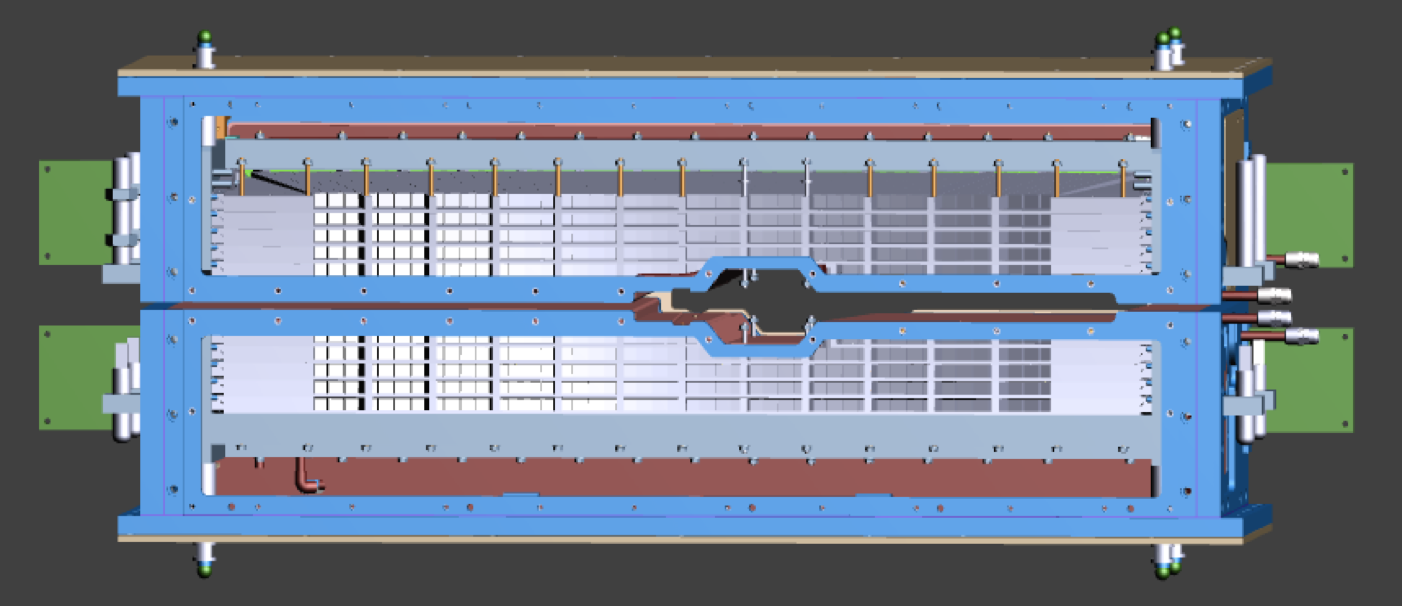
\includegraphics[width=0.85\textwidth]{pics/experiment/ecalface.png}
  \caption[Drawing of the ECal assembly face]{Drawing of the ECal assembly face, looking downstream along the beam direction. The ECal is assembled in two vertical halves and has a gap between allowing for the electron and photon beams. Beam electrons resulting from energy losses in the target are deflected in the dipole field toward the beam right and result in the ``sheet of flame". The ECal includes a cut out in order to avoid the high rates that result from detecting these particles.}
  \label{Figure:ecalface}
\end{figure}

\begin{figure}[h]
  \centering
      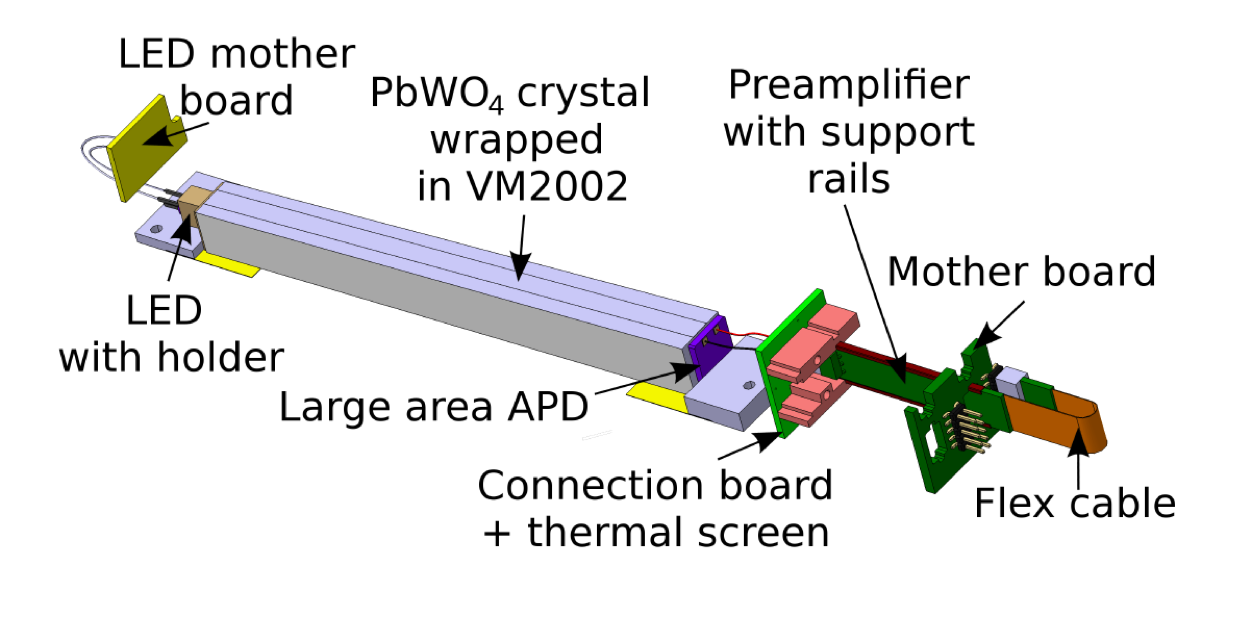
\includegraphics[width=0.85\textwidth]{pics/experiment/crystal.png}
  \caption[Single ECal module]{Drawing of an ECal crystal in readout configuration.}
  \label{Figure:crystal}
\end{figure}

\begin{figure}[h]
  \centering
      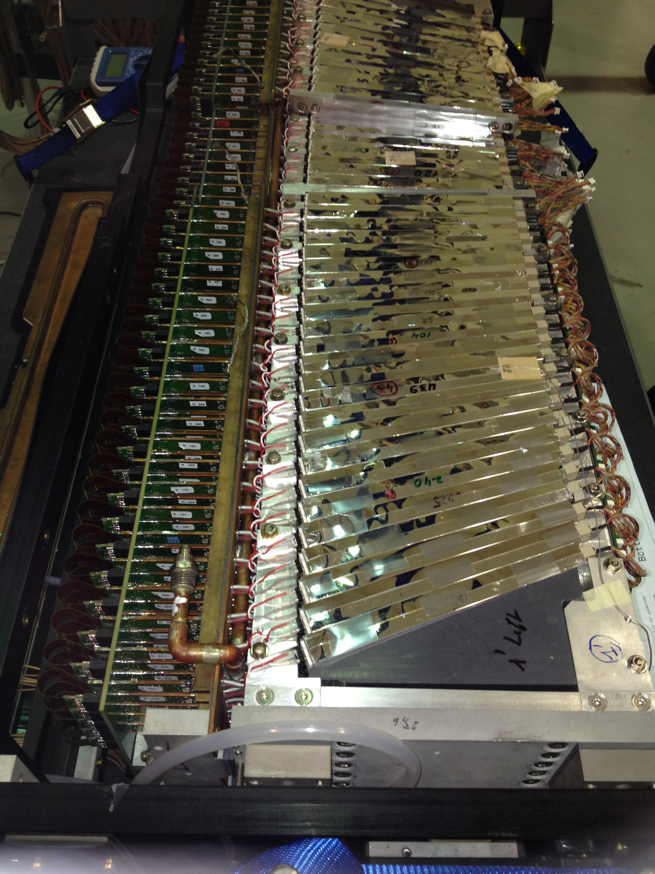
\includegraphics[width=0.5\textwidth]{pics/experiment/ecalAssembly1.png}
  \caption[Photograph of ECal crystals during assembly]{Photograph taken during assembly of the ECal from above. The preamplifiers attached to each crystal are shown on the left. As single layer of wrapped crystals are shown in their tray and the LEDs attached to each crystal are shown on the right.}
  \label{Figure:ecalAssembly1}
\end{figure}

Each crystal is wrapped in a VM2002 reflecting foil in order to increase light collection. The original APDs used by the the IC had a surface area of 5$\times$5~mm$^2$, but these were upgraded for HPS running by replacing each original APD with a large area APD (model S8664-1010) of surface area 10$\times$10~mm$^2$. The upgraded APDs collect four times more light than the old APDs. The larger signals require less electronic amplification of the signal and improve the signal-to noise-ratio. This allows a lower energy threshold for module readout and improves the energy resolution. \\
\indent The ECal is constructed as two separate vertical halves in order to avoid the 15~mrad vertical zone of excessive electromagnetic background along the beam line. The crystals in each half are arranged in five layers of 46 crystals. The layer of crystals closest to the beam in each half has nine crystals removed to allow for the passing of the unscattered electron beam. The two halves of the ECal are each at 2~cm from the  horizontal electron beam plane.\\
\indent As a particle enters the ECal, it initiates an electromagnetic shower by either bremsstrahlung or pair production. The secondary particles then produce more particles through bremsstrahlung and photon pair production giving rise to a cascade of particles, decreasing in energy. After the electron energy is too low to yield further particles, the remaining energy is deposited through ionization and excitation. The resulting scintillation photons hit the APD that converts the collected photons into an electronic signal via the photoelectric effect. Each APD is attached by a twisted pair connector to a preamplifier which converts the signal current to voltage and has low input impedence and noise.  



The gain of the APDs and the scintillation of the crystals in the ECal are temperature-dependent. An Anova A-40 external chiller operating at 17$\degree$C pumps cool water through copper cooling pipes that run along the inside of the ECal at the top, bottom, front and back faces of the structure. The internal temperature of the ECal was monitored using sixteen thermocouples located at various locations within the ECal. The thermocouples are read out using Omega D5000 series transmitters. Both devices are connected through RS-232 serial communications for external monitoring and alarms should the temperature change significantly.\\
\indent Low voltage power is supplied to the preamplifiers via an Agilent 6221 power supply operating at 5~V and approximately 4.1~A when all preamplifiers are connected. The high voltage to each of the 52 APD groups is supplied by CAEN A1520P modules in a SY4527 mainframe. Both voltage supplies are monitored and accessible for remote operations.  

\subsection{Light Monitoring System}
The Light Monitoring System (LMS) is a remotely-controlled upgrade to the ECal consisting of a bi-color LED attached to the front of each ECal module. PbWO$_4$ scintillating crystals are relatively radiation tolerant but have a known decrease in light yield after exposure to enough radiation~\cite{Batarin2005543}. This effect is non-uniform in the ECal as different modules are exposed to different levels of radiation. The LMS can turn individual modules on and off independently. This proved useful in checking each channel's functionality and correct cabling. The LEDs were selected such that the shape and duration of the emitted flash generates a pulse shape similar to the scintillation effect in the PbWO$_4$crystal~\cite{battaglieri_ft_clas12}.

Each crystal has a plastic LED holder glued to the front that contains a bi-color LED, model RAPID 56-0352, capable of emitting red and blue light. The use of two different colors allows for the study of different effects in the ECal modules. The blue LED has a wavelength close to the 430~nm emission peak of PbWO$_4$  \cite{battaglieri_ft_clas12} and is used to check for radiation damage in the crystal as this spectrum would be most affected. The red light is not sensitive to the radiation effects in the crystals, but is useful for checking the stability of the  APD gain. 

The LMS uses four driver boards on each half of the ECal. The four driver boards on each half are connected to one of two main controllers, and each driver can turn on a single LED at a time. The controllers communicate with the LMS through ethernet and USB interfaces. The controller board for the top half of the ECal also contains the master clock signal that sets the rate at which the LEDs flash. This clock signal is sent to the bottom controller so that the driver boards on the bottom half of the ECal can flash at the same rate, and the clock signal is used to trigger LED events when the DAQ is used. 


During the initial assembly of the ECal, the LEDs were used to study the cross talk between ECal modules. The cross talk between channels was found to be 2$\pm$1$\%$ and generally occurred in modules of the same row to the immediate left and right of the triggered module. The effect most likely appears due to light leakage out the back face of the crystal where the APD does not cover the entire surface.

The raw waveform response from a red LED signal in a single ECal module is shown in Figure~\ref{Figure:redSignal}. The raw units are given in mV which are a factor of four times less than the units of FADC.

\begin{figure}[htb]
  \centering
      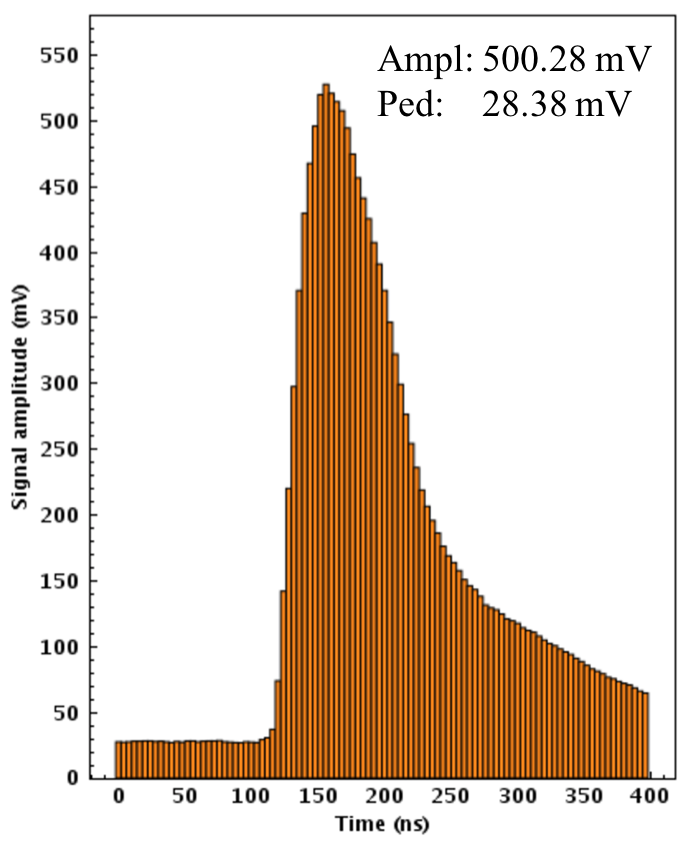
\includegraphics[width=0.5\textwidth]{pics/experiment/ledSignal.png}
  \caption[LED signal in ECal FADC]{A red LED in a single ECal module as readout through the FADC (see section~\ref{pulsefitting})}
  \label{Figure:redSignal}
\end{figure}

Before and after periods of long beam run times, the ECal gains were checked with the LEDs. The LED test ran a sequence of red and blue LED flashes so that the characteristic response of each module was measured. The typical results from an LED test are shown in Figure~\ref{Figure:redCompare}.

\begin{figure}[htb]
  \centering
      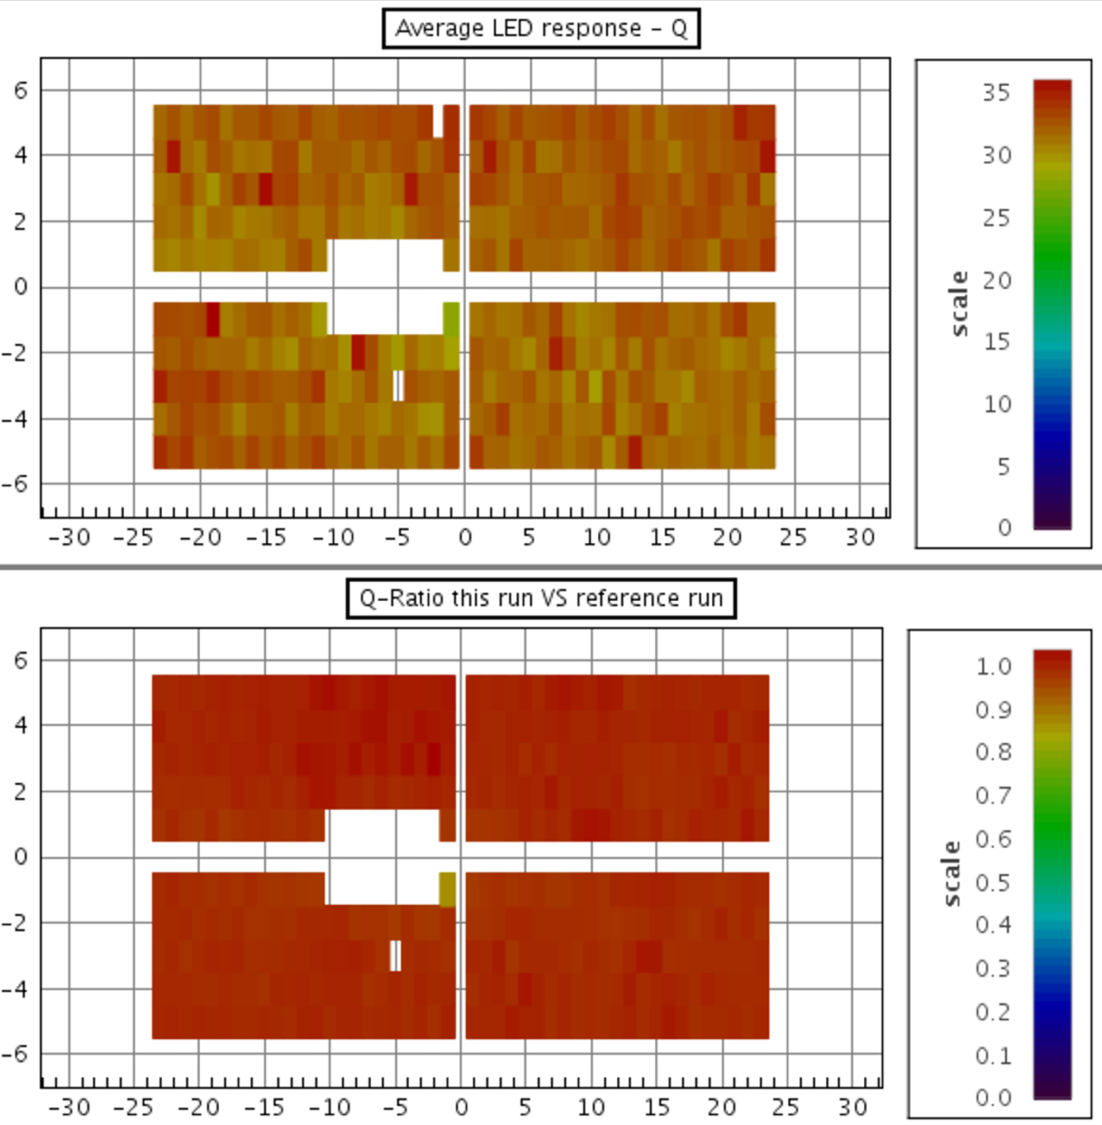
\includegraphics[width=0.65\textwidth]{pics/experiment/ledCompare.png}
  \caption[Results of a single LED run]{The top shows the LED response in each crystal for a specific LED run. The bottom compares each crystal with a its database value as stored from a previous LED run.}
  \label{Figure:redCompare}
\end{figure}

As shown in Figure~\ref{Figure:redCompare}, the individual ECal module response is given as the pulse-integral in units of GeV. The response values for individual crystals have large units of energy because the LED pulse is significantly longer than an actual scintillation pulse in the crystal. A LED test can show differences in the gain of individual crystals on the order of $1\%$ when compared to previous LED test results. During the Engineering Run, a 5$\%$ change in the gains across all modules occurred over the course of establishing production beam between February and April. This change was seen in LED response studies in addition to the gains obtained with cosmic energy calibration.

\subsection{Avalanche Photodiodes}


We upgraded the ECal by installing large area Hamamatsu S8664-3189 APDs for readout. APDs were used for reading out the ECal modules due to their ability to operate in the fringe magnetic field of the HPS beam line. Both the Institut de Physique Nucleaire d'Orsay (IPN) and Instituto Nazionale di Fisica Nucleare (INFN) groups in the HPS collaboration purchased the large area APDs for upgrade. As the IPN group re-designed the motherboards for the upgrade, INFN developed the testing apparatus so that the gain of each APD could be characterized and sorted into one of 52 high voltage groups to minimize response variations. The large area APDs are shown in Figure~\ref{Figure:apd}.

\begin{figure}[h]
  \centering
      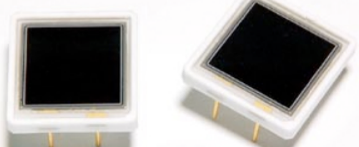
\includegraphics[width=0.4\textwidth]{pics/experiment/apd.png}
  \caption[Hamamatsu S8664-3189 large area APDs]{The Hamamatsu S8664-3189 large area APDs are $10\times10$~mm$^2$.}
  \label{Figure:apd}
\end{figure}

APDs are reverse-biased diodes with an internal high electric field that multiplies the electrons through an avalanche mechanism.  The characteristic gain of an APD depends on the temperature of the environment due to the interaction of the electrons with the phonons. The gain is inversely correlated with temperature.  The APD gains have a linear dependence on both voltage and temperature. Prior to grouping the APDs for installation in the ECal, each APD was tested and bench marked to check for quality and optimal operating voltage in order to achieve a pre-selected gain of 150. The testing apparatus was designed and installed by the group from INFN as the same procedure was used in the construction of the Forward Tagger~\cite{celentano_2014}. The apparatus is shown in Figure~\ref{Figure:apdtest}.

\begin{figure}[h]
  \centering
      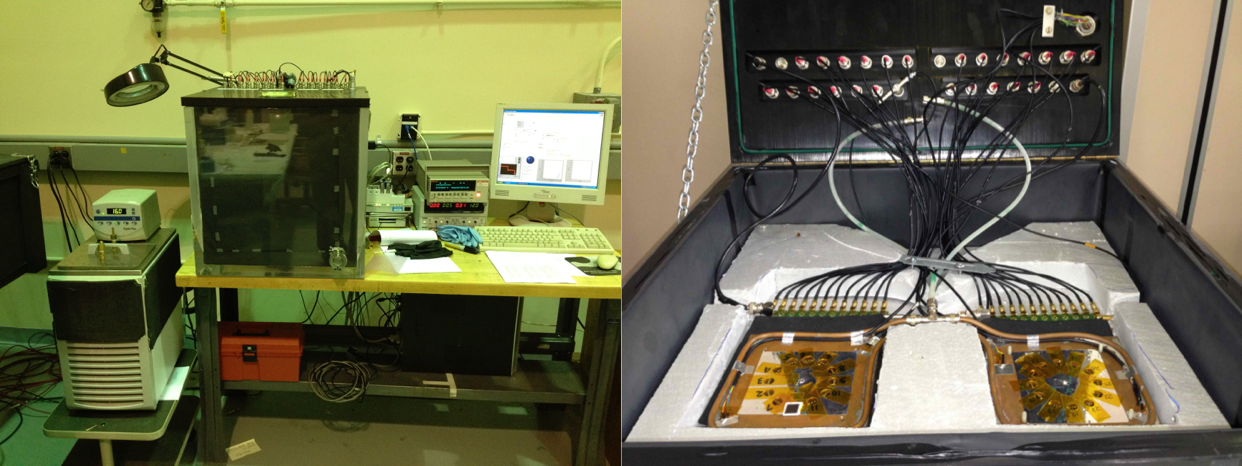
\includegraphics[width=0.7\textwidth]{pics/experiment/apdtests.png}
  \caption[Testing assembly for large area APDs]{On the left, the testing setup is shown and includes a chiller, the light-tight plastic box that contains the LEDs and APDs, an electrometer, and the data acquisition. On the right, the setup inside of the light-tight plastic box is shown that contains a copper cooling plate to maintain the chiller temperature, 10 slots on each side to hold APDs, and the LED in the center of each half.}
  \label{Figure:apdtest}
\end{figure}

In order to avoid condensation on the cooling lines, the temperature range for conducting the tests was limited to 16$\degree$C, 18$\degree$C, and 20$\degree$C. During the testing, the current in each APD is measured by the electrometer with the LED on and off while stepping through a range of voltages. The measured dark and light currents for an individual APD during testing are shown in Figure~\ref{Figure:apdcurrent}.

\begin{figure}[h]
  \centering
      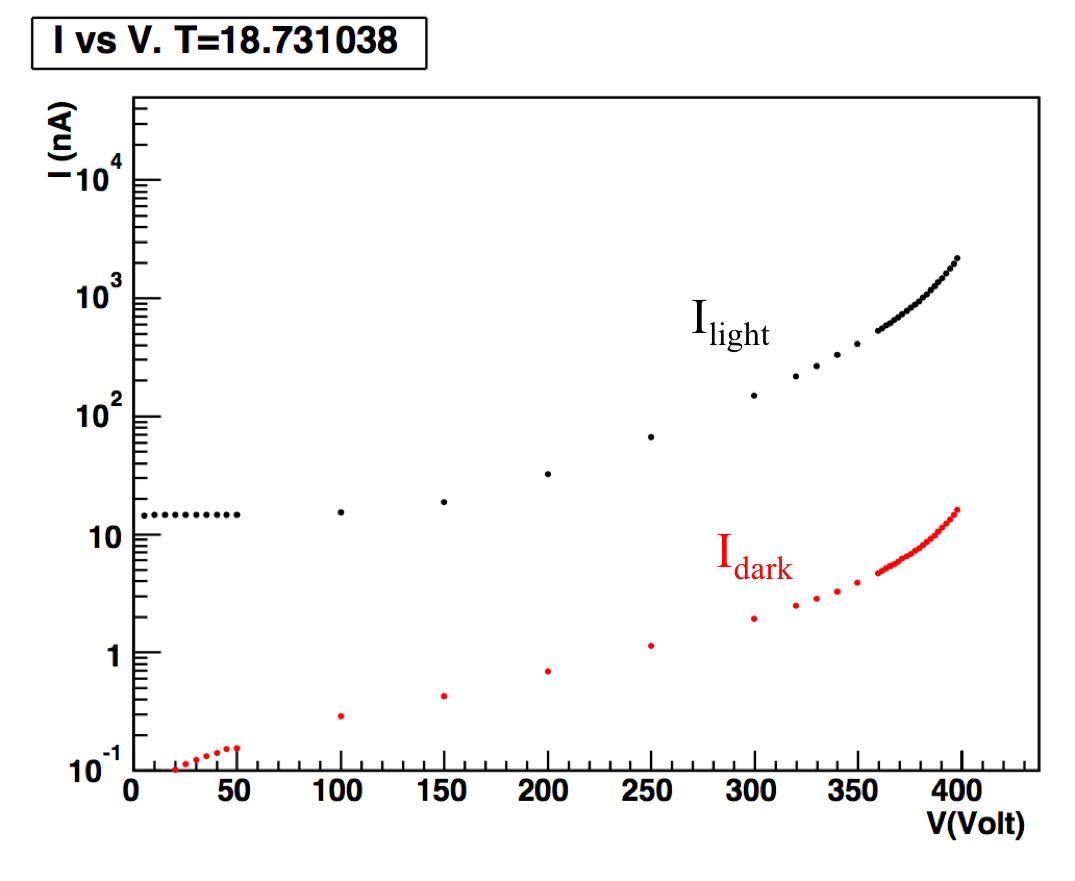
\includegraphics[width=0.5\textwidth]{pics/experiment/apdcurrent.png}
  \caption[APD current draw versus voltage with LED on and off]{The current measured from an individual APD as tested over a range of voltages with both the LED on and off. The measured temperature at the APD for this particular measurement was 18.7~$\degree$C.}
  \label{Figure:apdcurrent}
\end{figure}

The APD gain is calculated by the following relation:

\begin{equation}
	\label{eq:apdgain}
	Gain = \dfrac{I_{light}(V)-I_{dark}(V)}{I_{light}(G=1)-I_{dark}(G=1)} 
\end{equation}
The gain is 1 when the avalanche mechanism is not present. $I_{light}(G=1)$ in Eq.~\eqref{eq:gain} is the corresponding light current, and $I_{dark}(G=1)$ is the measured dark current when the gain is 1. Using this relation, the gain can be characterized for all measured dark currents and should have a linear relation. This relationship is shown in Figure~\ref{Figure:apdIvG}.

\begin{figure}[h]
  \centering
      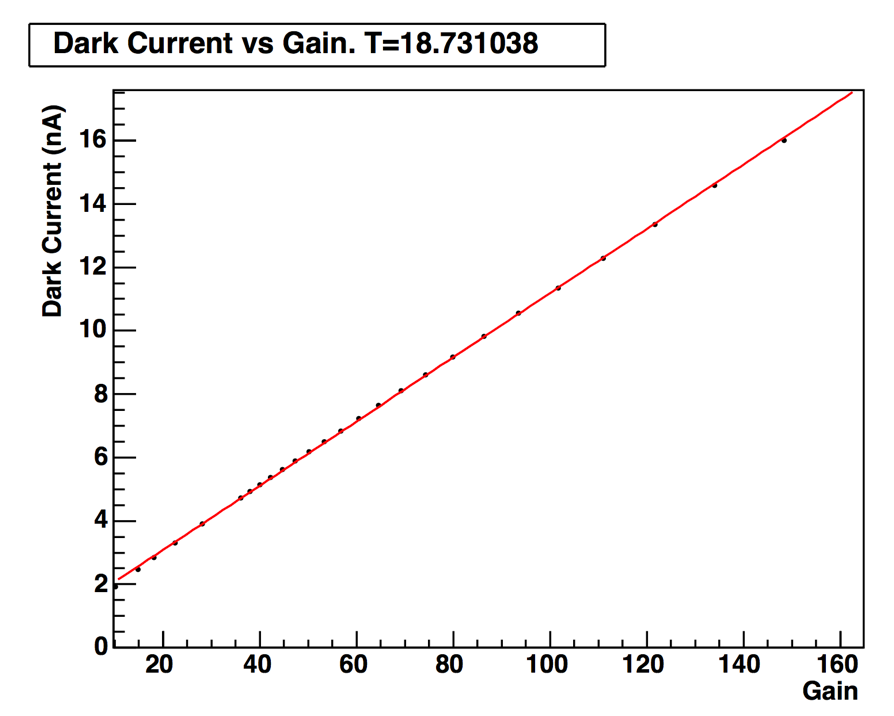
\includegraphics[width=0.5\textwidth]{pics/experiment/apdIvG.png}
  \caption[APD measured dark current as a function of gain]{The dark current measured from an individual APD plotted versus the gain as tested over a range of voltages with both the LED on and off. The measured temperature at the APD for this particular measurement was 18.7~$\degree$C.}
  \label{Figure:apdIvG}
\end{figure}

If the relationship between the dark current and the gain is not linear, as shown in Figure~\ref{Figure:apdIvG}, then the APD was re-tested to ensure quality. APDs were placed into 52 common voltage groups ranging from as little as two to a maximum of ten APDs in each group in order to minimize gain variations across the ECal. The grouping temperature was chosen to be 18~$\degree$C in order to avoid condensation in the cooling lines of the ECal. The optimal voltage for each APD at 18~$\degree$C and a pre-selected gain of 150 can be extrapolated as shown in Figure~\ref{Figure:apdTV}.

\begin{figure}[h]
  \centering
      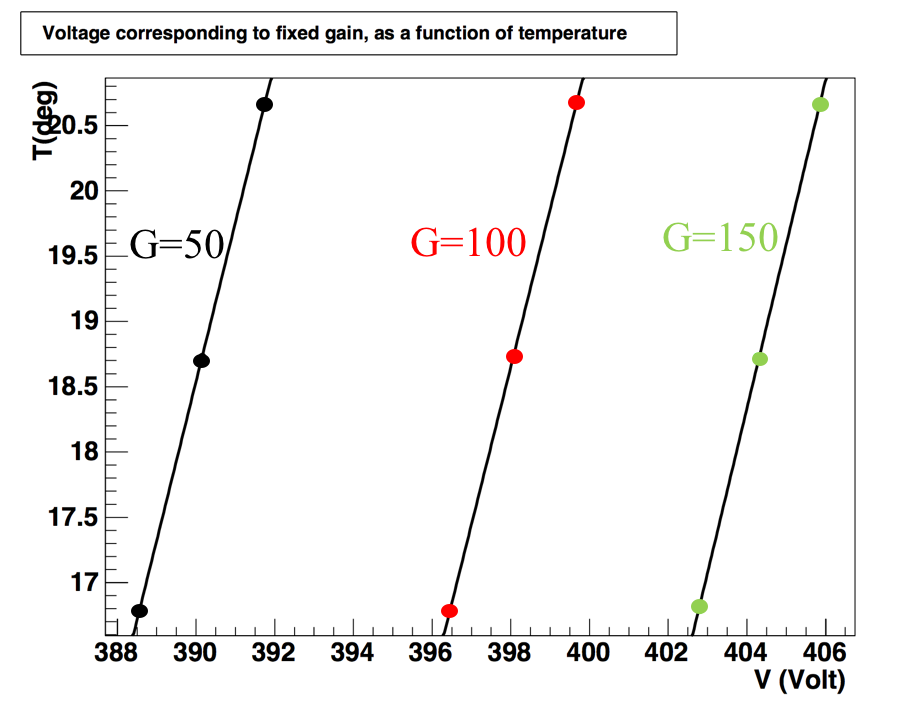
\includegraphics[width=0.5\textwidth]{pics/experiment/apdTV.png}
  \caption[APD fixed gain in terms of voltage and temperature]{The calculated voltages for fixed gains as a function of temperature can be used to group the APDs for common high voltage.}
  \label{Figure:apdTV}
\end{figure}

\section{Trigger}
Events of interest in the HPS experiment are triggered by the ECal. Each channel of the ECal is read out to an FADC250 with 16 channels per board. The FADC250 continuously samples analog signals at a rate of 250~MHz, or every 4~ns, with 12-bit precision. As the data size was small enough, the 2015 and 2016 data was recorded in raw mode such that 100~samples of raw information in a channel are read at the trigger time. This raw mode, called Mode 1, allowed for precise offline pulse fitting of the signals for optimal energy and timing resolution. In the 2015 Engineering Run, the signals from the ECal were split with $1/3$ of the signal going to TDCs and $2/3$ of the signal going to the FADCs. This was done as a precautionary measure in the event that the new FADCs were unreliable. In the 2016 Physics Run, the splitters were removed, allowing for the full signal to go to the FADC due to their proven capabilities. \\
\indent The full readout chain of the ECal trigger is shown in Figure~\ref{Figure:readoutChain}.
\begin{figure}[thb]
  \centering
      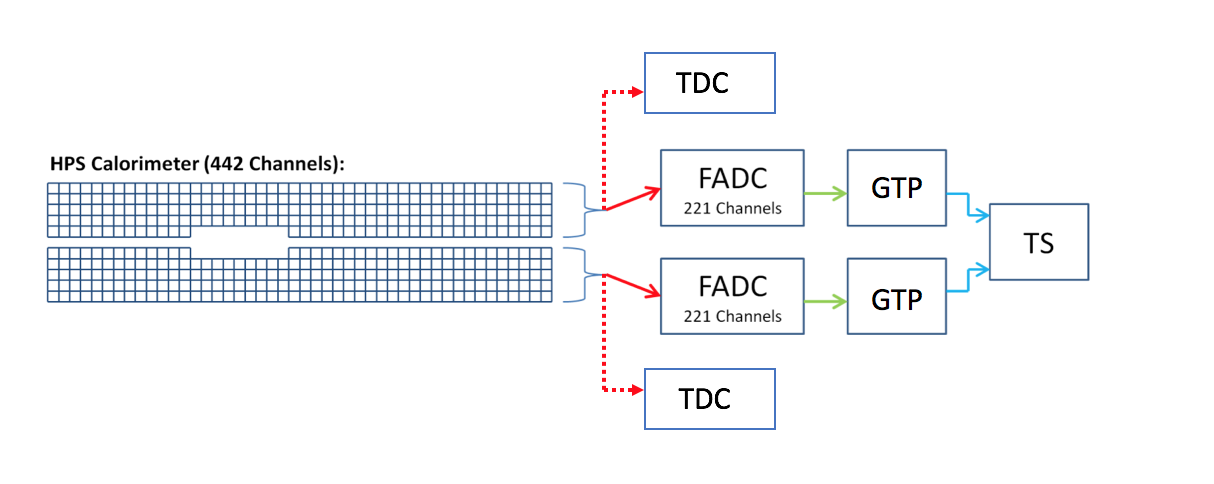
\includegraphics[width=0.75\textwidth]{pics/experiment/readoutChain.png}
  \caption[ECal readout chain]{The Flash ADC continuously samples ECal crystals at 250~MHz. In the 2015 Engineering Run, signals from the ECal were split with $1/3$ of the signal going to the TDCs and $2/3$ of the signal going to the FADCs. When a signal crosses threshold, the GTP makes $3\times3$ crystal clusters by searching for hits above threshold in adjacent crystals. The trigger processor (TP) uses the GTP clusters to make a trigger decision.}
  \label{Figure:readoutChain}
\end{figure}

When a signal crosses a pre-defined threshold, a set number of samples before and after the crossing are summed together to provide a pulse charge value which is converted to energy. The conversion to energy requires access to the individual channel gains and pedestals (as found by cosmic calibrations) which are pre-loaded into the data acquisition (DAQ) system. The energy and time of threshold crossing are sent to the General Trigger Processor (GTP) board every 16~ns  for clustering~\cite{balossino_hps_2016}\.\
\indent The GTP clusterer first identifies the crystal carrying the highest energy (known as the seed hit) in comparison to all surrounding crystals. The immediately neighboring crystals of the seed hit are compared in both energy and time coincidence with respect to the seed crystal in order to create a cluster. The cluster energy is the sum of all of the hits in a cluster. The timing coincidence is typically chosen to be 4~samples to allow for time-walk effects. The cluster information is then passed to the Subsystem Processor (SSP) to make a trigger decision based on various settable trigger cut requirements. \\
\indent The SSP includes several different trigger configurations that can run simultaneously containing different settable cuts and prescale values for ECal modules. The SSP looks for combinations of clusters that pass the configuration requirements and cuts and then sends a trigger to the Trigger Supervisor (TS) board when a cluster or pair of clusters satisfies the trigger requirements. The trigger is then sent to the Trigger Interface (TI) boards in order to trigger readout of all detectors.\\ 
\indent The SSP trigger configurations include two different cluster-pair triggers, two different single-cluster triggers, a random pulser trigger, a cosmic trigger, and an LED trigger of which all except for the cosmic and LED triggers were run during data taking with beam. The first single cluster trigger, Single-1, was optimized for elastically-scattered beam energy electrons off the target. The looser version of the trigger was Single-0. These triggers were useful in selecting events for calibrating the ECal and studying the trigger efficiencies. The cluster-pair trigger is the primary trigger for the HPS experiment and studies all possible combinations of clusters in the ECal for pair selection. It requires one cluster in each half of the ECal. The tuneable cuts used in this trigger are presented in Table~\ref{tab:pairTriggerCuts}~\cite{balossino_hps_2016}. \\

\begin{table}[htb]
\caption{Pair-1 Trigger Cuts}
\label{tab:pairTriggerCuts}
\centering
\begin{tabular}{lc}
\toprule
%\multicolumn{2}{c}{Name} \\
%\cmidrule(r){1-2}
Trigger cut & Cut value \\
\midrule
Time difference & $| t_{top}-t_{bot} | \leq t_{coincidence}$   \\
Cluster energy & $E_{min}<E_{i}<E_{max}$\\
Cluster sum & $E_{sum min}\leq E_1+E_2\leq E_{sum max}$\\
Cluster size & $N_{hits}\geq N_{threshold}$\\
Energy difference & $ E_{2}-E_{1}<E_{difference}$\\
Coplanarity & $ |\arctan\dfrac{x_1}{y_1}-\arctan\dfrac{x_2}{y_2} | \leq \theta_{coplanarity}$\\
Energy-distance & $E_{1}+r_{1}F\geq E_{slope}$ \\ 
\bottomrule
\end{tabular}
\end{table}

The variables $t_i,E_i, N_i, x_i,$ and $y_i$ denote the cluster time, cluster energy, number of hits in the cluster, and coordinates of the cluster, respectively. The subscript, $1$, denotes the cluster with the lowest energy of the pair.  The parameter, $r_1$, is the distance between the center of the lowest energy cluster and the center of the ECal (defined as $r_1=\sqrt{x_1^2+y_1^2}$). The parameters selected for the cuts include the $t_{coincidence}, E_{min}, E_{max}, E_{sum min}, E_{sum max}, N_{threshold}, E_{difference}, \theta_{coplanarity}, r_{1},$ and $E_{slope}$, and are chosen from studying A$^{\prime}$ Monte Carlo in order to optimize the signal acceptance while minimizing the background. The GTP clusters are created prior to track-matching and offline clustering (which includes hits belonging to a cluster beyond those immediately adjacent to the seed hit). For the 2015 data, a GTP cluster conserves roughly 80$\%$ of the fully reconstructed particle energy when the seed hit is not on the edge of the ECal. \\
\indent The time coincidence cut is kept loose enough in the SSP pairs cluster selection to allow for time walk and cabling offsets which are not corrected for until the full pulse is fitted in offline reconstruction. At the GTP stage, the time only corresponds to threshold crossing. The cluster energy cut selects clusters that are reconstructed by the GTP in the energy range of interest. The minimum hit requirement for clusters was lowered at the start of running due to $A^{\prime}$ Monte Carlo studies indicating that 1 hit clusters were possible and could improve reach without overburdening the trigger. The cluster sum cut most significantly removes accidental pairs containing elastically-scattered beam energy electrons in addition to removing low energy cluster sum events that will not pass thresholds for well-reconstructed events. The energy difference cut removes events that have extremely different cluster energies and do not satisfy $A^{\prime}$-type criteria. \\
\indent The coplanarity cut removes events that are not coplanar including M$\o$ller and wide-angle bremsstrahlung (WAB) backgrounds because the $e^+e^-$ trident events of interest are distributed symmetrically around the beamline. The angle is calculated from the center of the ECal where the beam line passes through to each cluster in the pair relative to the vertical axis. The pairs should be approximately $180\degree$ apart. \\
\indent The energy-distance cut is applied to the lowest-energy cluster of the pair in order to reject events where the cluster is too close to where the electron beam passes through the ECal. Trident kinematics show that these clusters are dominated by bremsstrahlung low energy photons and that there is some reasonable distance of separation with respect to the beamline for these lower energy events.\\ 
\indent The cut values used in the 2015 Pair-1 trigger are shown in Table~\ref{tab:pairTriggerVals}.

\begin{table}[htb]
\caption{Pair-1 trigger cut values for the Engineering Run}
\label{tab:pairTriggerVals}
\centering
\begin{tabular}{lc}
\toprule
%\multicolumn{2}{c}{Name} \\
%\cmidrule(r){1-2}
Trigger cut & Cut value \\
\midrule
Time difference & $| t_{top}-t_{bot} | \leq12$ ns   \\
Cluster energy & $54<E<630$ MeV \\
Cluster size & $N_{hits}\geq 1$\\
Energy sum & $180<E_{top}+E_{bot}<860$ MeV\\
Energy difference & $| E_{top}-E_{bot}|<540$ MeV\\
Coplanarity & $\theta_{top}-\theta_{bot}<30\degree $\\
Energy-distance & $E_{1}+(5.5 \textrm{ MeV/mm})r_{1}>600$ MeV\\ 
\bottomrule
\end{tabular}
\end{table}

\indent The pulser trigger generates a constant rate of triggers at 100~Hz regardless of the physics events as measured by the ECal. This makes the pulser an unbiased probe for measuring the backgrounds of the experiment during running with the beam and concurrent with other triggers.\\ 
\indent The cosmic trigger was used without the beam for calibration of the ECal and uses the timing coincidence between two scintillators, placed below and external to the ECal, in order to trigger readout of all ECal channels for offline reconstruction of the cosmic event. The timing coincidence of the scintillators placed in line and below the ECal was chosen to be 40~ns where the leading edge of the scintillator signal in the FADC pulse crosses 60~ADC samples. Once the timing and threshold conditions are met, all modules in the ECal were readout in Mode 1 format. 

%%%%%%%%%%%%%%%%%%%%%%%%%%%%%%%%%%%%%%%%%
\chapter{Detector Calibration and Performance} 
%The ECal was installed in Hall B in the fall of 2014 and then calibrated using cosmic ray energy deposition in the crystals. The ECal was fully commissioned with a 2~GeV electron beam in December 2014 and demonstrated that the electronics read out chain from the ECal worked. The SVT was installed in the spring, and both detectors were calibrated using the data obtained from the 1.056~GeV electron beam in the 2015 engineering run. This chapter describes the methodology for calibration and the performance of the SVT and the ECal in the HPS experiment. 

\section{Silicon Vertex Tracker Performance}
The SVT measures particle hit locations on its silicon strips and reconstructs particle trajectories. The SVT momentum calibration strongly depends on the accuracy of its alignment in the magnetic field. In offline analysis, pairs of tracks are re-fit to obtain the vertex location. The invariant mass of the pair is reconstructed from the vertex of the two tracks by using the measured opening angle and the momenta. 

\subsection{Track reconstruction}

Hits in the SVT strips have an associated amplitude and time reported from the fit to the raw spectrum. These fitted hits are then clustered on the strips. The highest amplitude hit on the strip is designated as the ``seed" hit and must pass a threshold amplitude of $4\sigma_{noise}$. Hits on surrounding strips that are above $3\sigma_{noise}$ and within 8~ns of the seed time are added to the cluster. The position of the cluster is calculated using an amplitude-weighted position, and the time of the cluster is calculated as an amplitude-squared weighted time of the hits in the cluster~\cite{uemura_search_2016}. These are considered to be the 1D hits on the sensor. \\
\indent These 1D hits are converted into 3D hits by pairing the 1D hits with a cluster on the other sensor associated with that layer. These 1D hits are matched as coming from the same particle if they are close enough spatially such that the strips cross and if they are within 16~ns of each other. If they pass these cuts, then a 3D hit is created at their point of intersection. The 3D hit position is calculated from the track fit to these two hits because there is some small angle and distance between the two pair sensors.\\
\indent The initially constructed tracks are called seed tracks. Candidate seed tracks are first built by fitting a helix to hits in three SVT layers. These layers are considered to be the layers that ``seed" that track. The track is then extrapolated to a fourth layer which searches for a hit near the track that ``confirms" the track, and the track is re-fit to include this hit. If no hit is found, the track is discarded. Seed tracks that have been seeded and confirmed are then ``extended" to test for hits consistent with the track in the fifth and sixth layers. Only one hit layer is required to extend the track, but the track can match to hits in both layers. The designation of which specific layers are used for seeding, confirming, and extending tracks is the tracking strategy. During the 2015 engineering run, HPS used four different tracking strategies so that no track combination would be overlooked. Seed tracks that pass the strategy criteria are fit with a single helix to all the hits. The effects of multiple scattering are propagated with the position resolution at the downstream layers to reduce their importance in the fit.\\
\indent General Broken Lines (GBL) is a model that is used for the final track fitting that fully accounts for the effects of multiple scattering at each layer~\cite{blobel_fast_2011}~\cite{kleinwort_general_2012}. GBL treats each track as a series of track segments connected by scatters in each silicon sensor. A full GBL track fit is optimized to reduce the position residuals of each hit on the track and to minimize the kinks in scattering angles at each sensor on the track. Because each scatter is treated independently at each layer, scatters in downstream layers do not significantly alter the track trajectory upstream. GBL tracks are used for HPS analysis. 

\subsection{Momentum resolution}
The momentum resolution of the SVT is determined at the beam energy separately for the top and bottom by looking at tracks from elastically-scattered electrons. The momentum resolution of these tracks indicate the momentum resolution at the beam energy of 1.056~GeV. 

\begin{figure}[thb]
  \centering
      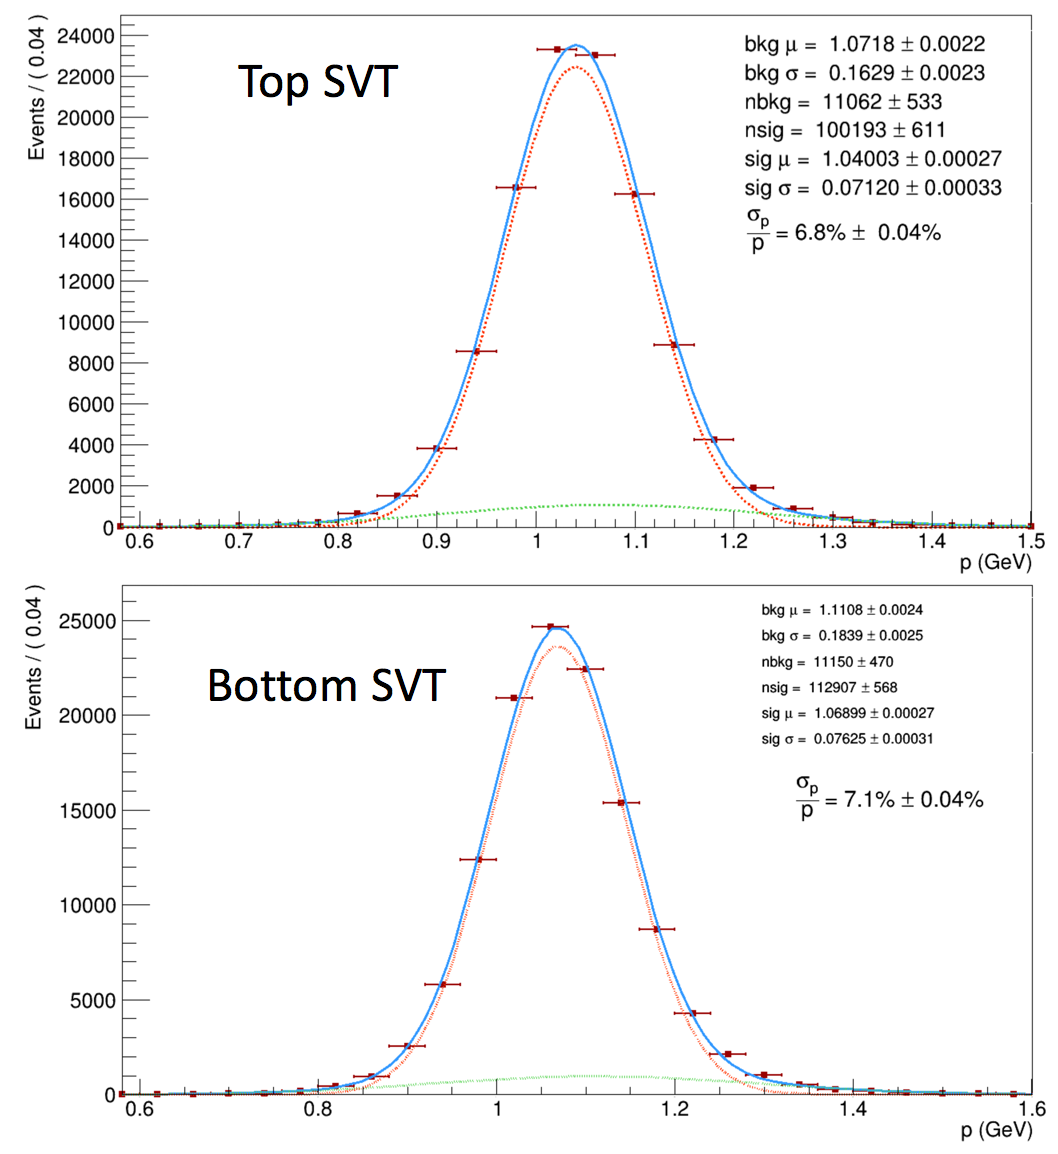
\includegraphics[width=0.75\textwidth]{pics/performance/SVTMom.png}
  \caption[Momentum resolution of the SVT]{The momentum resolution for elastically-scattered electron tracks passing through the top and bottom halves of the halves of the ECal separately. The momentum resolution is approximately 7$\%$~\cite{moreno_search_2016}.}
  \label{Figure:pRes}
\end{figure}

By using the measured ECal energy and resolution (see discussion in section~\ref{EcalResData}), one can also extract the momentum resolution of the SVT for different track momenta. By looking at tracks matched to clusters in the ECal and fitting the ratio of the measured ECal energy $E$ to the SVT momentum $P$ distribution, the momentum resolution is extracted as
\begin{equation}
	\label{eq:pres}
	\sigma_P = P\sqrt{\sigma_{E/P}^2-\Big(\dfrac{\sigma_E}{E}\Big)^2} 
\end{equation}
where $\sigma_{E/P}$ is the measured width of the $E/P$ distribution fit with a Gaussian, and $\sigma_E/E$ is the energy-dependent ECal energy resolution. The SVT momentum resolution is roughly 7$\%$ across the range of momenta accessible in the 2015 run configuration (see Figure~\ref{Figure:pResExtrap}). The momentum resolution is within 0.5$\%$ of the resolution found by fitting the SVT elastically-scattered electron tracks shown in Figure~\ref{Figure:pRes}.

\begin{figure}[thb]
  \centering
      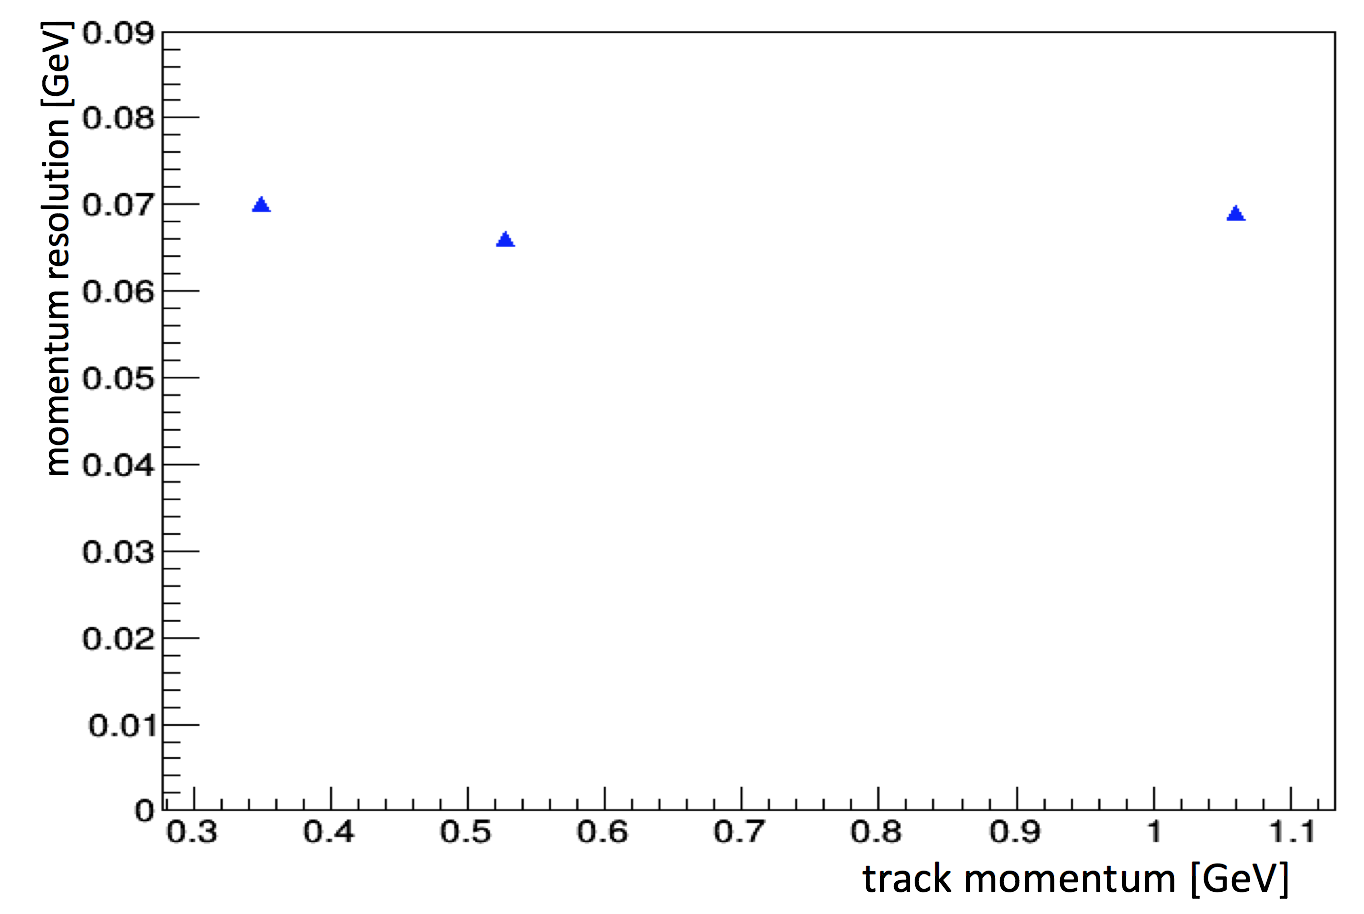
\includegraphics[width=0.75\textwidth]{pics/performance/pResExtrapolated.png}
  \caption[Momentum resolution of the SVT extracted from $E/P$]{The momentum resolution of the SVT is roughly constant for all accessibly momenta at 7$\%$. This is roughly consistent with the momentum found in Figure~\ref{Figure:pRes}.}
  \label{Figure:pResExtrap}
\end{figure}

\subsection{Tracking efficiency}

Reconstructed GBL tracks require a minimum of five hit tracks but can have six hit tracks. The tracking efficiency per SVT layer is extracted from the ratio of six-hit tracks to the number of five or more hit tracks missing a certain layer. It is better than 98$\%$ for layers 2--5. Layer 1 has the lowest efficiency of all the tracking layers at around 90$\%$ as shown in Figure~\ref{Figure:trackEff}. The inefficiency of Layer 1 is thought to be due to the high rates from being close to the active beam. 

\begin{figure}[thb]
  \centering
      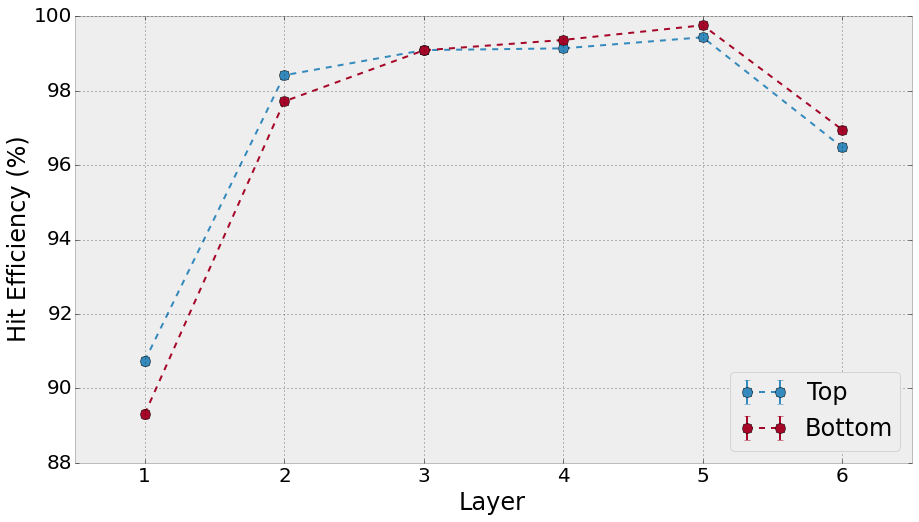
\includegraphics[width=0.75\textwidth]{pics/performance/engrun2015_hit_efficiency_vs_layer.png}
  \caption[Tracking efficiency of the SVT by layer]{The tracking efficiency is shown by layer as a comparison between the number of six-hit tracks and the number five or more hit tracks missing a particlular layer. The tracking efficiency is generally high (better than 95$\%$), but Layer 1 is lower than the other layers at  90$\%$~\cite{moreno_search_2016}.}
  \label{Figure:trackEff}
\end{figure}

\subsubsection{Tracking efficiency using three particle events}
We can also measure the overall tracking efficiency of the SVT by using three particle final state events. These may result from tridents or wide angle bremsstrahlung pair conversion. These events require three clusters in the ECal and two or more tracks. The three clusters are chosen to ensure that they come from events with three particles. For any two SVT tracks, the third track must have a projected momentum that would have passed through the SVT. For events with three tracks, the momentum sum (as shown in Figure~\ref{Figure:psumtrks}) reflects the quality of the selection criteria. 
\begin{figure}[thb]
  \centering
      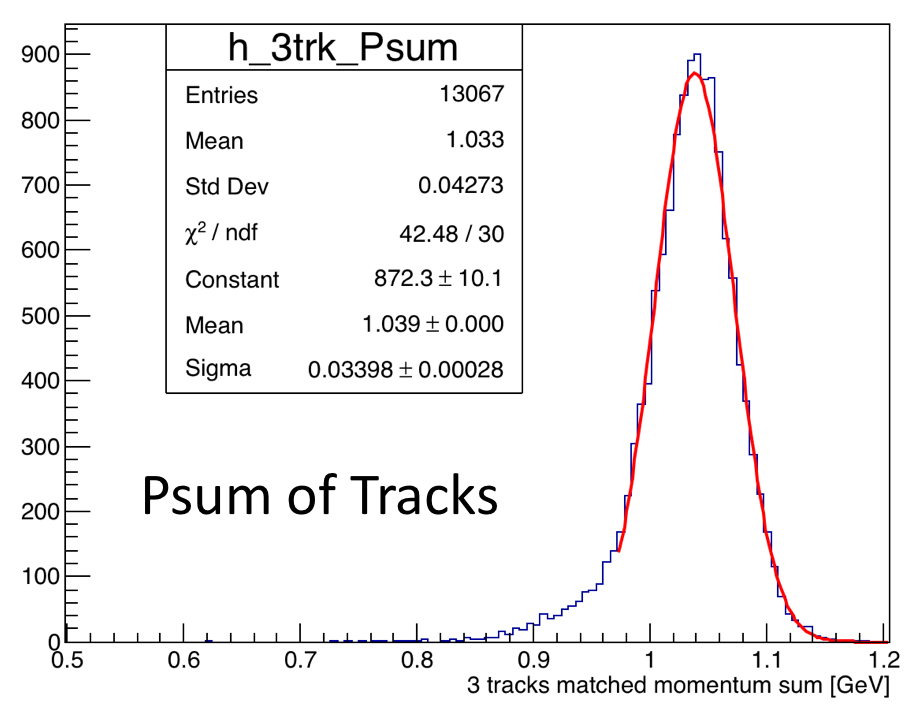
\includegraphics[width=0.55\textwidth]{pics/performance/pSum_3trk.png}
  \caption[Momentum sum of three track final state particles]{The momentum sum of three track final state particles is shown.}
  \label{Figure:psumtrks}
\end{figure}

The combined cluster energy sum was required to be within 10$\%$ of the beam energy so as to eliminate events that did not contain three particles. The ratio of the number of three track events to the number of two or more track events tells us the efficiency of measuring a certain particle. This technique is limited to measuring the efficiency at low momentum ($<0.5$~GeV/c).\\
\indent There are three different topologies considered for each particle type ($e^+$ or $e^-$): whether it was in a half (top or bottom) by itself, in the half with the electron that is closest to the beamline, or in the half with the electron that is farthest from the beamline. The efficiencies for these topologies were found to be the same for particles in the top versus the bottom so those results were combined to improve statistics. Bins with low statistics were thrown out. The efficiencies can be seen in Figure~\ref{fig:eff3prong}.


\begin{figure}[hbt]
%\begin{center}
\begin{minipage}{0.55\textwidth}
	  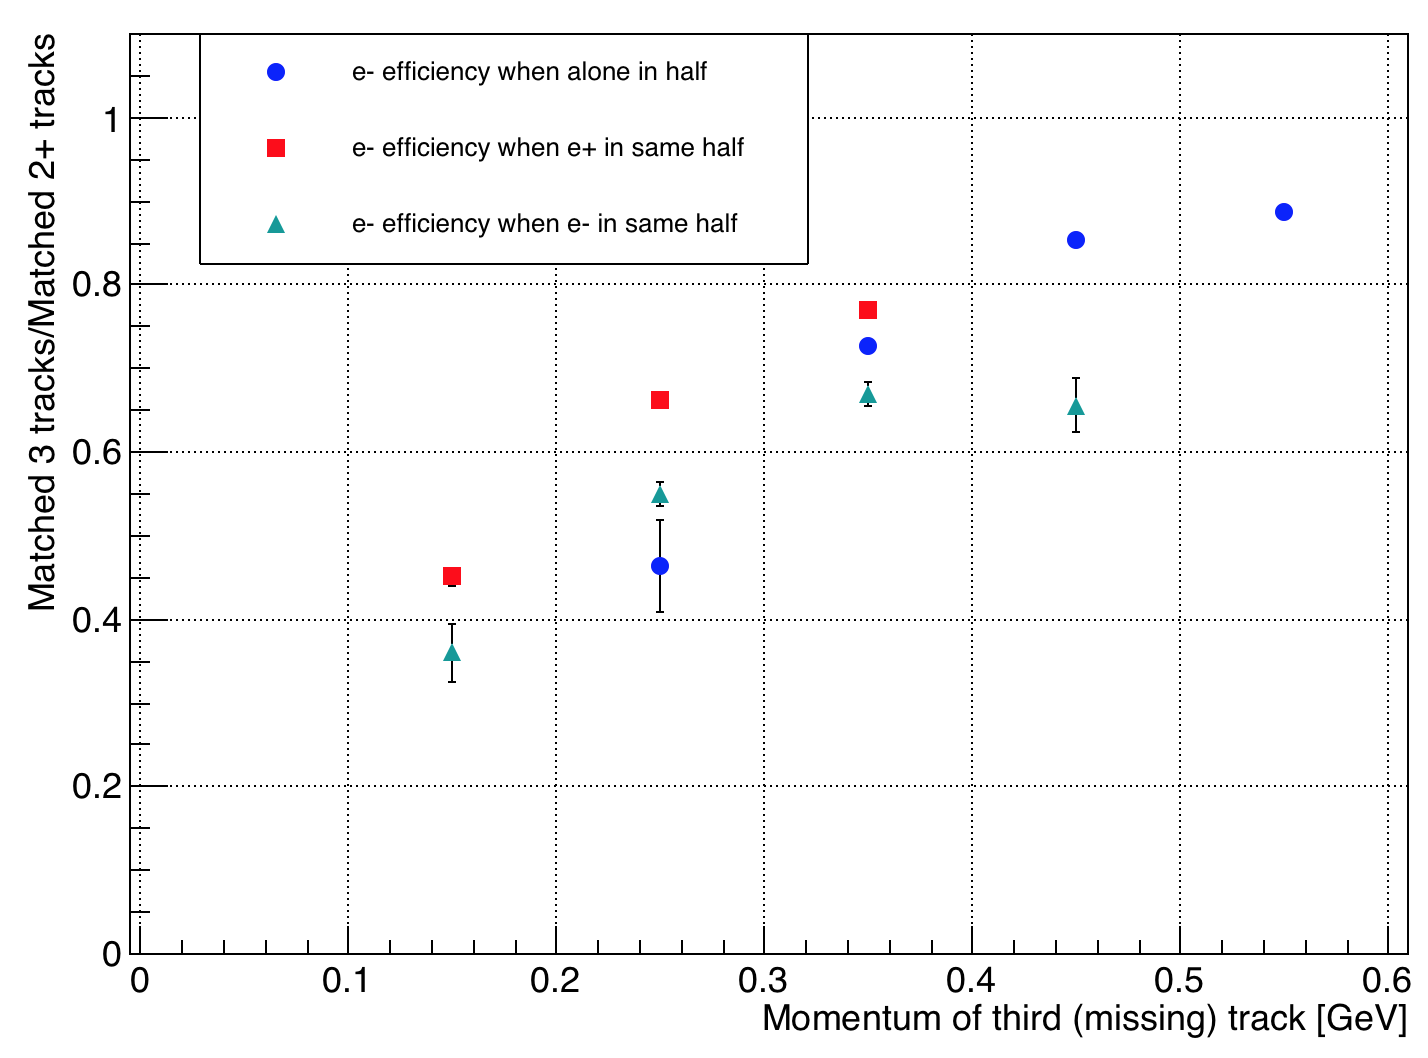
\includegraphics[width=\textwidth]{pics/performance/em_trkEff.png}
    	  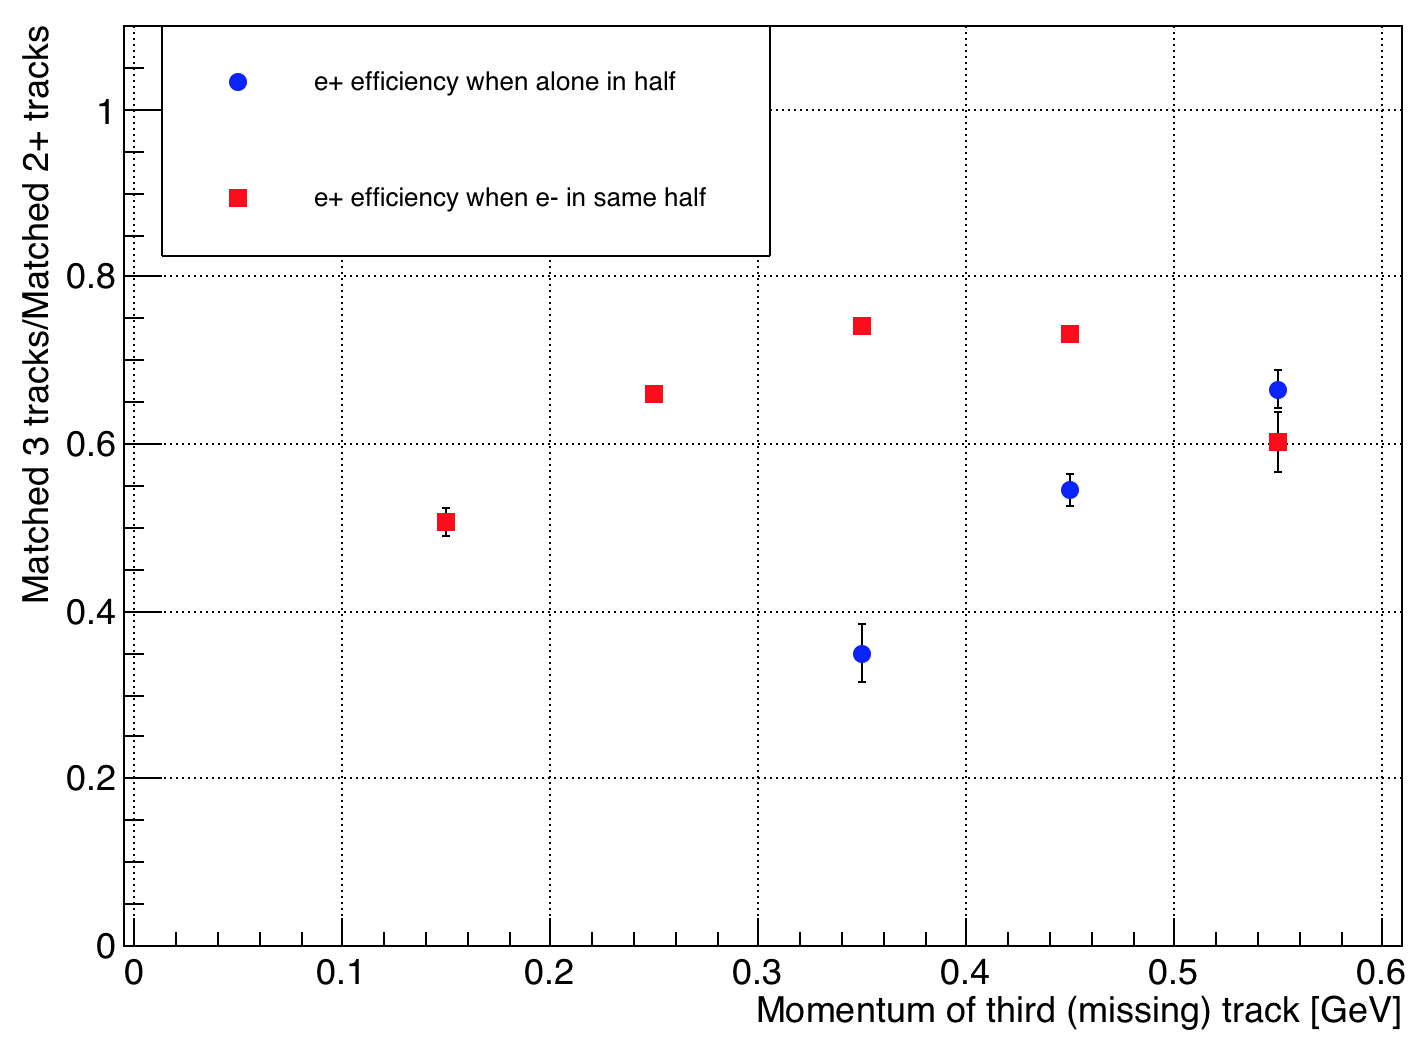
\includegraphics[width=\textwidth]{pics/performance/ep_trkEff.png}
%\end{center}
\end{minipage}\hfill\begin{minipage}{0.32\textwidth}
\caption[Tracking efficiency from three particle final state events]{ \label{fig:eff3prong} \baselineskip 11pt
{The efficiency for tracking a particle as a function of its momentum. The tracking efficiency for electrons (top) and positrons (bottom) is shown separately for different topologies.}
}
\end{minipage}
\end{figure}

The resulting electron efficiency increases with momentum and plateaus around 400~MeV. This turn on of the efficiency was not previously seen in the trident Monte Carlo. The positron efficiency is more difficult to interpret and has yet to be fully understood. The positron spectrum may be more influenced by the pair-converted wide angle bremsstrahlung. The general tracking efficiency assumed in the proposal was 0.85. 

%%%%%%%%%%%%%%%%%%%%%%%%%%%%%%%%%%%%%%%%%%%%%%%%%%%
\section{Electromagnetic Calorimeter}
The ECal was calibrated both in energy and time. The first calibration performed before receiving beam from the accelerator was the cosmic ray energy calibration. A full timing calibration of the ECal was performed using the accelerator RF signal and cluster-pair events. A final calibration using physics events from elastically-scattered beam energy electrons and events from wide angle bremsstrahlung (WAB) yielded the full calibration of the ECal for all energies.  

\subsection{Energy Reconstruction}
The ECal uses an adapted version of the clustering algorithm that was used by the CLAS IC. The geometrical arrangement of the crystals differs greatly from that used by the IC and required detailed studies and simulations to reconstruct the incident particle energy. The angles of incidence of the particles (electrons, positrons, and photons) entering the ECal varies significantly across the ECal. The edge effects in the ECal are substantial due to the horizontal split between the top and bottom halves and  the proximity to the beam. \\
\indent As a particle enters the ECal, it deposits all of its energy in the crystal material. Due to the segmentation of the calorimeter, multiple adjacent crystals will each contain different fractions of the incident particle's energy. In offline clustering, the energy is reconstructed by summing all of the modules that measured some amount of the incident particle energy. The total reconstructed energy is always proportional to and less than the incident particle energy due to energy loss effects. These energy loss effects can best be studied through simulation and experimental testing with the electronics.\\
\indent Clustering searches for a crystal having energy higher than all the immediately adjacent modules. This module becomes the ``seed" hit and initializes the cluster. The clustering algorithm then searches for hits surrounding the seed hit with lower energy and adds these hits to the cluster.The process continues by searching for hits surrounding the clustered hits with lower energy to add to the cluster. When two clusters overlap such that it is difficult to identify which hit a cluster belongs to, the energy of that module is divided between the two clusters in proportion to the seed hit energies of the two clusters.  Once all hits have been clustered, the cluster energy is the summed energy of all of the hit contributions within the cluster. 

\subsubsection{Simulations}
Simulations were performed using the fully modeled detector geometry in SLIC as part of the standard HPS software package. The geometry includes all strips of the SVT, vacuum chambers, ECal crystals, and relevant dead material. The software also tracks particles through a 3D magnetic field map corresponding to the field values for 1~GeV beam running~\cite{szumila-vance_hps_2016}.\\
\indent Single electrons, positrons, and photons were simulated at discrete energies of 0.2, 0.3, 0.4, 0.5, 0.6, 0.7, 0.8,  0.9, 1.0, and 1.1~GeV to uniformly cover the range of energies detectable in the 2015 engineering run. The simulation uses the full reconstruction chain excluding pile-up effects. Offline reconstruction clusters all of the adjacent ECal crystals containing some fraction of the incident particle energy so that the total cluster energy can be measured as the sum of the energy carried by all of the crystals in a cluster. The offline cluster reconstruction uses the same thresholds used in data and production Monte Carlo: 7.5~MeV for individual hits, 50~MeV for seed hits in clusters, and 100~MeV for cluster energies.\\
\indent Due to the complex showering cascade that occurs when a particle deposits its energy in the ECal, several adjacent crystal modules contain some fraction of the incident energy of the particle. These modules are clustered in offline reconstruction to obtain the total deposited energy of the incident particle. The reconstructed energy, $E_{rec}$, not corrected for shower loss effects is 

\begin{equation}
\label{eq:eclsum}
E_{rec} = \sum_i E_i    
\end{equation}
where $E_i$ is the energy of the $i^{\textrm{th}}$ module in the cluster. Some energy is lost between crystals and out the back of the ECal. After summing the ECal energy over the cluster, the incident particle energy can be found by correcting for the shower loss effects as  

\begin{equation}
\label{eq:eclsf}
E_{corr} = \dfrac{E_{rec}}{f}   
\end{equation}
where $f$ is the energy-dependent ratio of measured to incident particle energy. This factor is obtained from simulation. The energy loss corrections as derived from Monte Carlo are shown in Figure~\ref{Figure:ecorr}.

\begin{figure}[thb]
  \centering
      \includegraphics[width=0.75\textwidth]{pics/performance/energycorrection.pdf}
  \caption[ECal energy shower correction functions derived from simulation]{The fraction $f$ is the reconstructed cluster energy, $E_{rec}$, divided by the Monte Carlo generated particle energy, $E_{gen}$, and is plotted versus the reconstructed energy. Each simulated particle type is shown in a different color, and the functional fit of Equation~\eqref{eq:ecorrfunc} for each particle is shown by the dashed lines.}
  \label{Figure:ecorr}
\end{figure}

The difference in the energy corrections for the various particle types arises from geometrical effects and the incident angles of the particles entering the crystals~\cite{szumila-vance_hps_ecal_2014}. The focal point of the calorimeter, the point toward which all crystals are angled, lies 80~cm from the front face of the ECal. The HPS target is beyond this focal distance at approximately 1.4~m from the face of the ECal and is offset beam right in the pair spectrometer magnetic field. Charged particles produced at the target take different trajectories from the target to the ECal due to the magnetic field. This affects the entry angle of the particle into a crystal and requires a charge and momentum-dependent correction. The form of the energy correction function for the central region of the ECal is described by a three parameter fit:\\

\begin{equation}
	\label{eq:ecorrfunc}
	\dfrac{E_{rec}}{E_{gen}} = \dfrac{A}{E_{rec}}+\dfrac{B}{\sqrt{E_{rec}}}+C 
\end{equation}

The shower leakage effects in crystals becomes significant close to the calorimeter edge. The energy reconstruction deteriorates rapidly in the crystals closest to the edge but is relatively constant in central region of the ECal. The energy reconstruction at the edges was characterized using Monte Carlo as a function of particle hit position in the ECal relative to the inner beam gap edge. In Equation ~\eqref{eq:ecorrfunc}, parameter $A$ is not strongly correlated with position and remains constant for a given particle type. Parameters $B$ and $C$  strongly depend on the cluster position relative to the beam gap edge of the ECal. These dependencies can be seen for electrons in Figure~\ref{Figure:sfparEdge}.

\begin{figure}[htb]
  \centering
      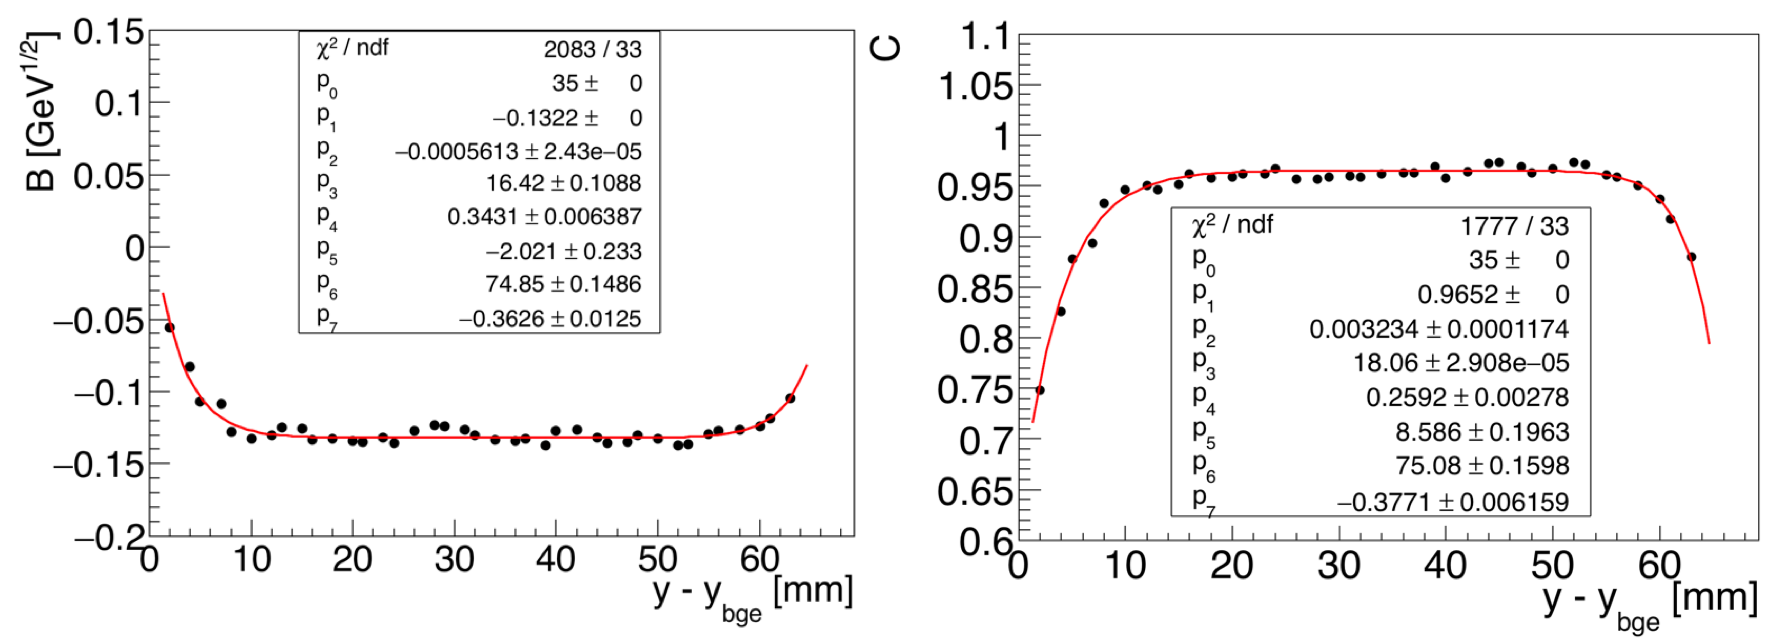
\includegraphics[width=1.0\textwidth]{pics/performance/sfparEdgeFit.png}
  \caption[ECal energy shower parameters for electrons relative to the inside beam gap edge]{Parameters $B$ and $C$ from Eq.~\ref{eq:ecorrfunc} for electrons, as a function of vertical position
relative to the innermost beam gap edge.}
  \label{Figure:sfparEdge}
\end{figure}
The energy leakage parameters $B$ and $C$ can be fit with two functions at the edges that match in the central region of the ECal, away from the edges of the calorimeter. The equations used to fit the $B$ and $C$ parameters are described by:

\begin{equation}
\begin{split}
\label{eq:p1parlt}
B(y<p_0) = p_1-p_2 e^{-(y-p_3)p_4}\\
B(y>p_0) = p_1-p_5 e^{-(y-p_6)p_7}
\end{split}
\end{equation}

\begin{equation}
\begin{split}
\label{eq:p2parlt}
C(y<p_0) = p_1-p_2 e^{-(y-p_3)p_4}\\
C(y>p_0) = p_1-p_5 e^{-(y-p_6)p_7}
\end{split}
\end{equation}

The energy leakage correction functions are relatively constant in the central region of the calorimeter and are matched at a central distance $p_0$. For columns containing 5 crystals, the distance to the beam gap edge is the absolute value of the distance from the cluster centroid to the innermost beam gap edge. In the regions above and below the region where row 1 crystals are removed in the ECal, additional consideration is made when calculating the distance to the inner beam gap edge in order to be consistent with other regions of the ECal. At distances within 35~mm to the inner beam gap edge of row 2 when above and below the electron hole, the distance to the inner beam gap edge for the corrections corresponds to the inner edge of the row 2 crystals. At distances greater than 35~mm from the inner beam gap edge above and below the electron hole, the correction is applied relative to the inner beam gap edge distance as calculated to the inner edge of the row 1 crystals. This ensures that the edge corrections are consistent throughout the different regions of the ECal. For completeness, the corresponding energy correction parameters for positrons and photons are seen in Figures~\ref{Figure:sfparEdgeEP} and \ref{Figure:sfparEdgeP}, respectively. 

\begin{figure}[htb]
  \centering
      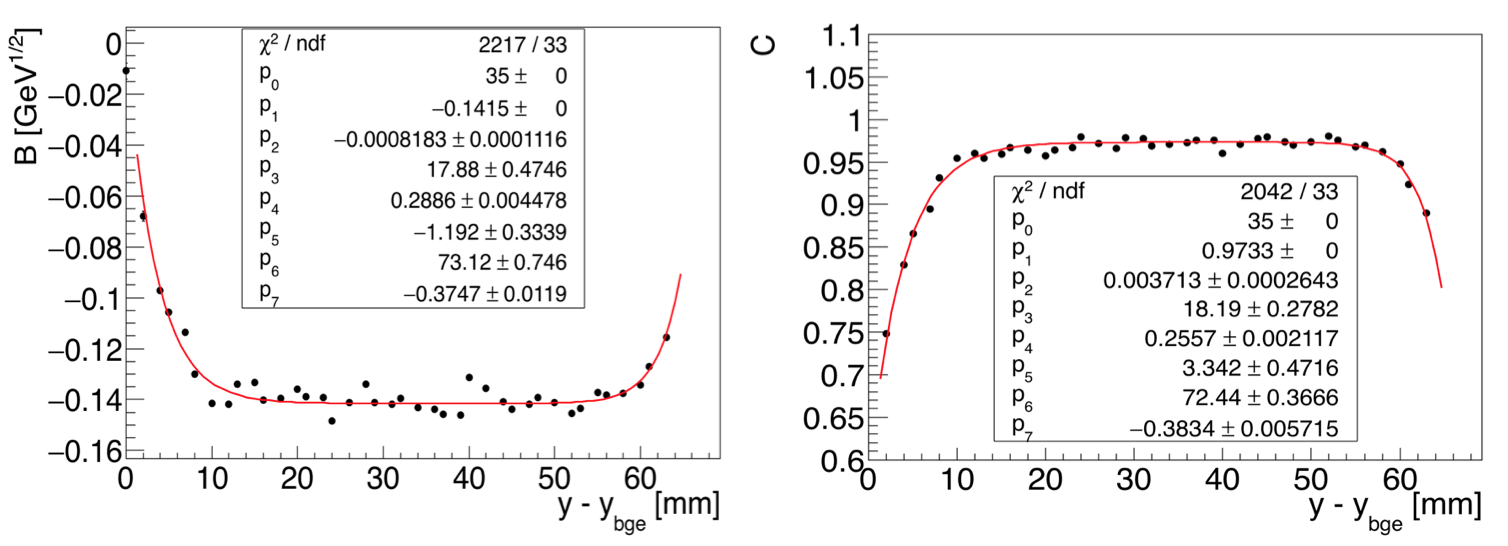
\includegraphics[width=1.0\textwidth]{pics/performance/sfparEdge_ep.png}
  \caption[ECal energy shower parameters for positrons relative to the inside beam gap edge]{Parameters $B$ and $C$ from Eq.~\ref{eq:ecorrfunc} for positrons, as a function of vertical distance from the innermost beam gap edge.}
  \label{Figure:sfparEdgeEP}
\end{figure}

\begin{figure}[htb]
  \centering
      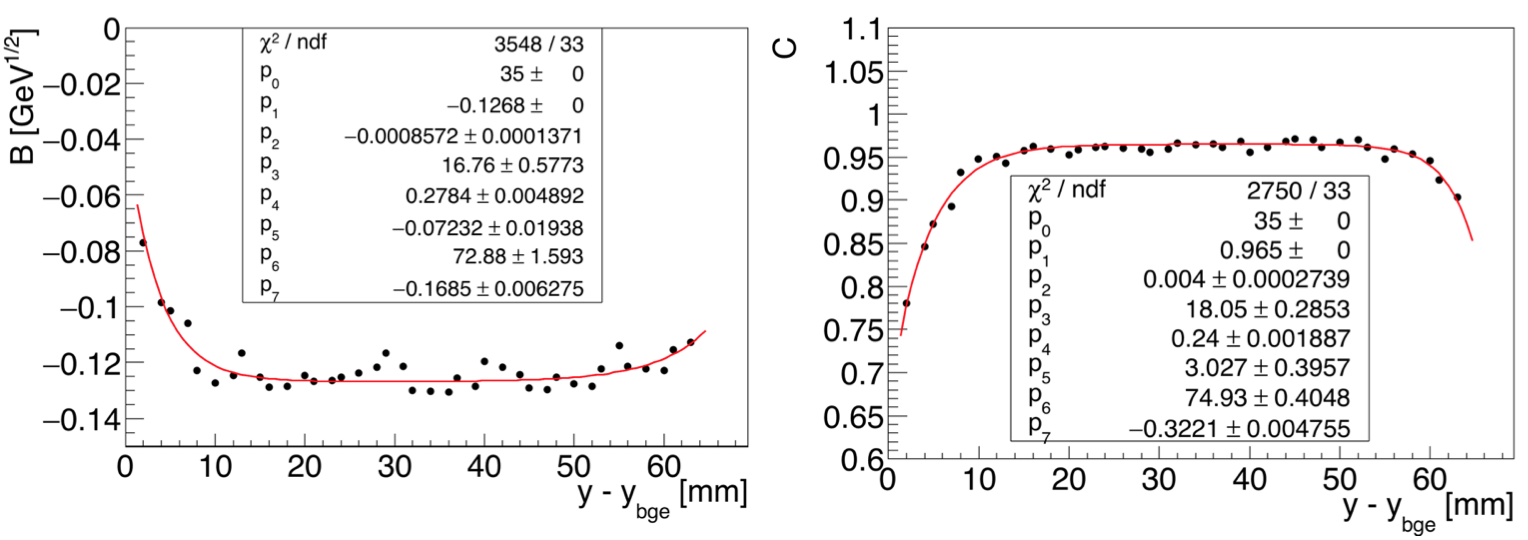
\includegraphics[width=1.0\textwidth]{pics/performance/sfparEdge_p.png}
  \caption[ECal energy shower parameters for photons relative to the inside beam gap edge]{Parameters $B$ and $C$ from Eq.~\ref{eq:ecorrfunc} for photons, as a function of vertical position
relative to the innermost beam gap edge.}
  \label{Figure:sfparEdgeP}
\end{figure}

The energy correction fraction is relatively constant beginning at approximately 1~cm from the ECal edges. As a result, we define the fiducial region of the ECal to be more than 1~cm from the edge, or approximately 3/4 of the front face crystal dimension. This result is consistent with the findings for the CLAS IC~\cite{szumila-vance_hps_ecal_2014}.\\
\indent In reconstruction of the data, the energy of all the crystals in the cluster are summed to make the uncorrected, reconstructed cluster energy. Separately, tracks from the SVT are matched with clusters in the ECal. From the curvature of the track, the particle type can be determined as being either a positron or electron. Clusters that have no matching track are determined to be due to photons. The position of the track at the ECal and the particle type are used to apply the corrections in Equation~\eqref{eq:ecorrfunc} that contain the further edge corrections (if necessary) from Equations~\eqref{eq:p1parlt} and~\eqref{eq:p2parlt}. Photon clusters are corrected using the photon-type energy and position corrections to the cluster in the ECal.  

\subsubsection{Energy resolution}

The energy resolution of the ECal is energy-dependent and improves with energy as approximately $1/\sqrt{E}$. 
\begin{figure}[htb]
  \centering
      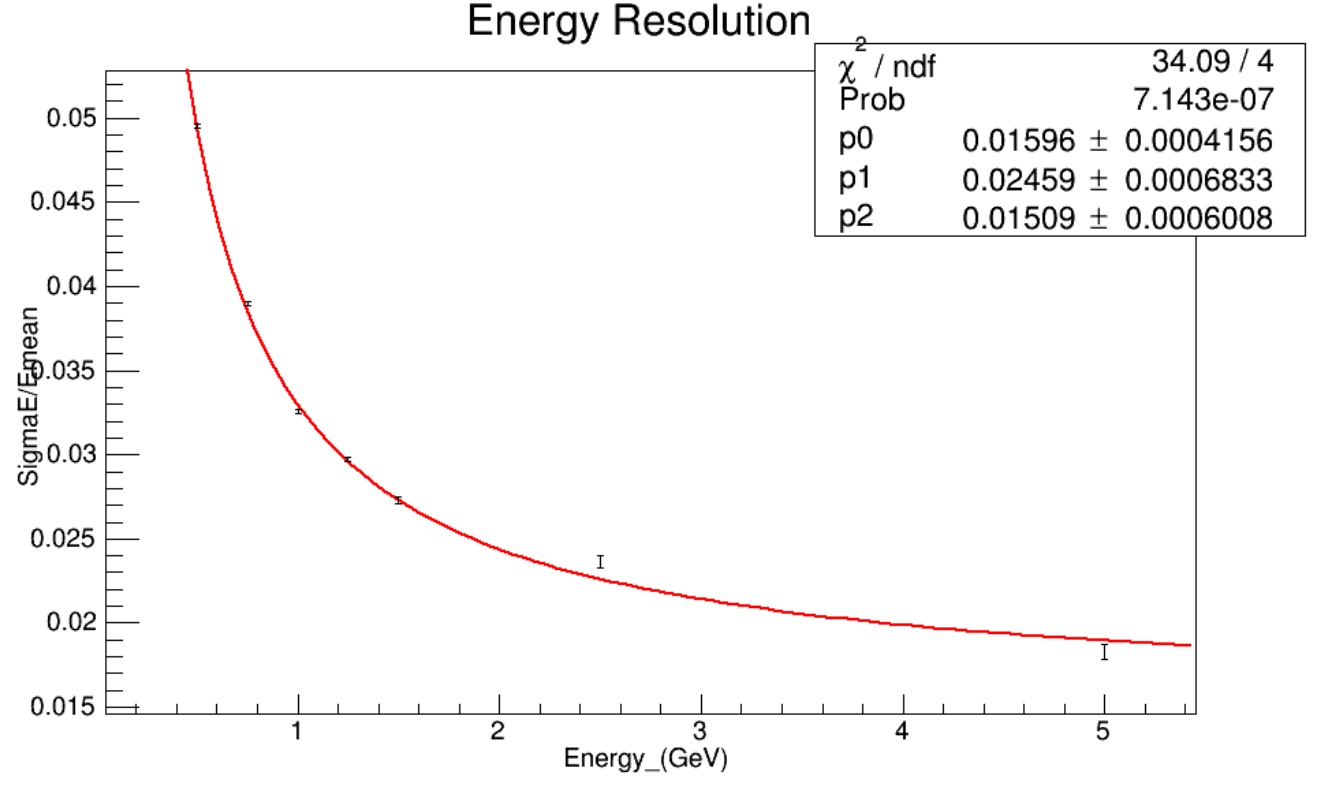
\includegraphics[width=0.6\textwidth]{pics/performance/eResFitMC.png}
  \caption[ECal fractional energy resolution fitted from simulation]{ECal fractional energy resolution from simulation. The points show the fractional energy resolution extracted from simulation, and the red line is the fit to the points.}
  \label{Figure:eResFitMC}
\end{figure}
From simulation, we obtain the energy resolution as shown in Figure~\ref{Figure:eResFitMC}. The fit shown in Figure~\ref{Figure:eResFitMC} is described by
\begin{equation}
\label{eq:eResMC}
\dfrac{\sigma_E}{E} (\%) = \dfrac{1.60}{E} \oplus \dfrac{2.46}{\sqrt{E}} \oplus 1.51
\end{equation}
where the energy is in units of GeV. The first term corresponds to the preamplifier noise. We were expecting 3~MeV$\times \sqrt{10} = 0.009$~GeV, where 10 is the average number of hit crystals, but we instead measured 0.016~GeV. Simulation does not include the FADC error (expected to be 1.3~MeV~\cite{charles_2014}) which contributes a term (in $\%$) as $0.13\sqrt{10}\textrm{ [GeV]}/E\textrm{ [GeV]}$ which must be added quadratically to the first term. The second term corresponds to the statistical fluctuations in the shower development and is influenced by the lateral containment of the shower and energy deposited in the crystals. The second term from simulation does not include fluctuations in the number of photoelectrons (30 photoelectrons/MeV, multiplied by an excess noise factor parameterizing the fluctuations in the APD gain process, or Fano factor, of 2~\cite{panda_2008}) contributing $0.8/\sqrt{E}$. This term is calculated as $\sqrt{F/N_{pe/GeV}}$. The third term is interpreted as the fluctuation of energy leakage through the back of the crystals. This third term should include the crystal-to-crystal inter-calibration error which is estimated to be 1$\%$~\cite{szumila-vance_hps_ecal_2014}. By including these additional resolution effects in the measurement, we obtain the resolution as anticipated from Monte Carlo

\begin{equation}
\label{eq:eResUpdated}
\dfrac{\sigma_E}{E} (\%) = \dfrac{1.65}{E} \oplus \dfrac{2.59}{\sqrt{E}} \oplus 1.81 
\end{equation}
where the energy is in units of GeV.

\subsubsection{Position reconstruction}
\indent ECal clusters can provide position information of comparable resolution to the SVT. Weighting schemes for calculating the cluster centroid must avoid periodic patterns resulting from the crystal segmentation. The CLAS IC algorithm provided the optimal position resolution:~\cite{szumila-vance_hps_ecal_2014}

\begin{equation}
\begin{split}
\label{eq:posncalc}
x_{cl} & =  \dfrac{\sum_i w_i x_i}{\sum_i w_i}\\
y_{cl} & =  \dfrac{\sum_i w_i y_i}{\sum_i w_i}
\end{split}
\end{equation}
where $x_i$ and $y_i$ are the $x$ and $y$ positions of the $i^{\textrm{th}}$ crystal in the cluster, and the crystal weight $w_i$ is described by 

\begin{equation}
\label{eq:posnwt}
w_i  =  \max[0, w_0+\ln\dfrac{E_i}{E_{rec}}]
\end{equation}
Here, $E_i$ is the energy deposited in the $i^{\textrm{th}}$ crystal, $E_{rec}$ is the sum of the energies of all of the crystals in the cluster, and $w_0$ is an energy threshold such that $E_i/E_{rec} > e^{-w_0}$ and is found in simulation to have a value of $3.1$~\cite{szumila-vance_hps_ecal_2014}. The logarithmic term enhances the contribution from the tails and improves the position measurement.\\
\begin{figure}[htb]
  \centering
      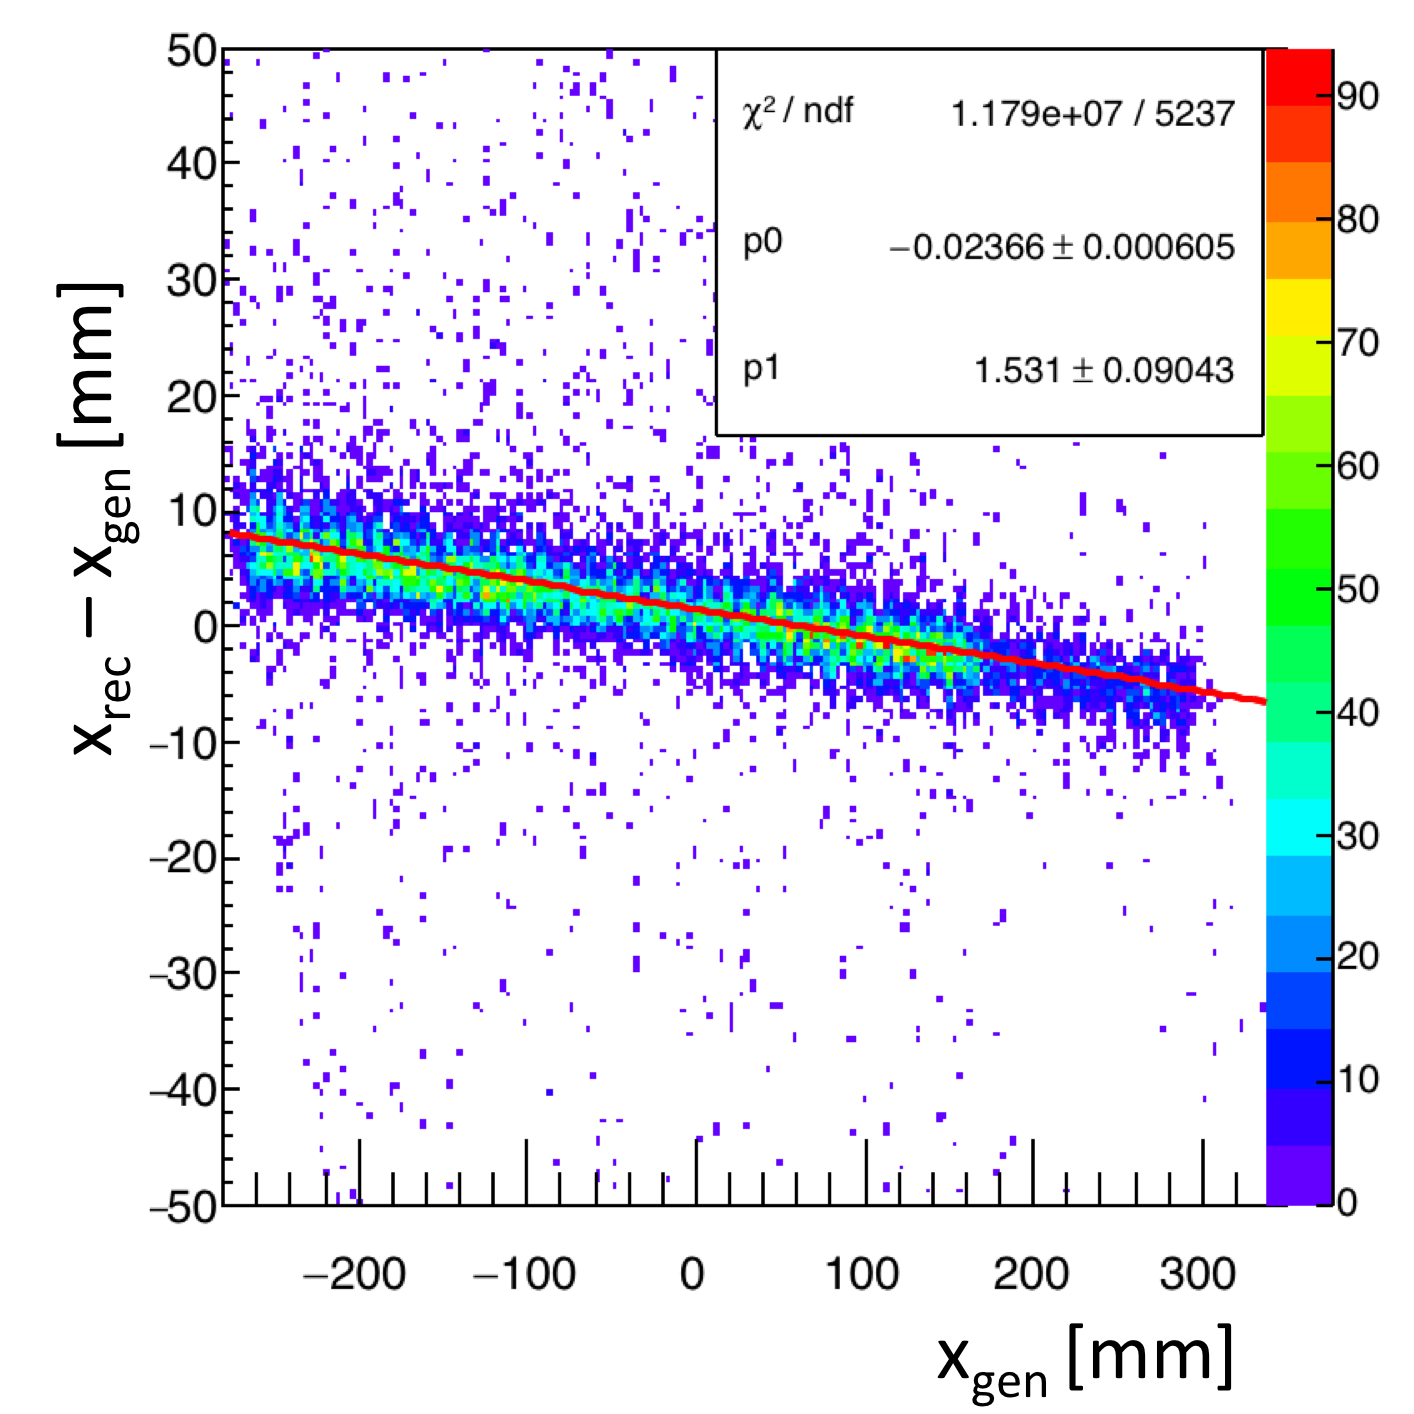
\includegraphics[width=0.7\textwidth]{pics/performance/xposn1gev.png}
  \caption[Horizontal position correction for 1~GeV electrons]{The position correction for 1~GeV electrons plotted versus the Monte Carlo generated position at the ECal. It is both energy and position-dependent in order to account for the different angles of incidence at the ECal.}
  \label{Figure:xposn1gev}
\end{figure}
\indent Additional effects resulting from the differing angles of entry at the ECal require a position correction to the $x$-coordinate of the cluster. These corrections are both charge and momentum-dependent. The position correction for a generated 1~GeV electron is shown in Figure~\ref{Figure:xposn1gev}. The correction at each energy by particle-type is fit with
\begin{equation}
\label{eq:posncorr}
x_{rec} - x_{gen} = A(E_{rec}) x_{gen} + B(E_{rec})
\end{equation}
where the energy-dependence of the fit parameters $A(E_{rec})$ and $B(E_{rec})$ uses the reconstructed cluster energy, uncorrected for shower loss effects. These parameters for the electron horizontal position correction as a function of the reconstructed cluster energy are shown Figure~\ref{Figure:xposcorrPar}.

\begin{figure}[htb]
  \centering
      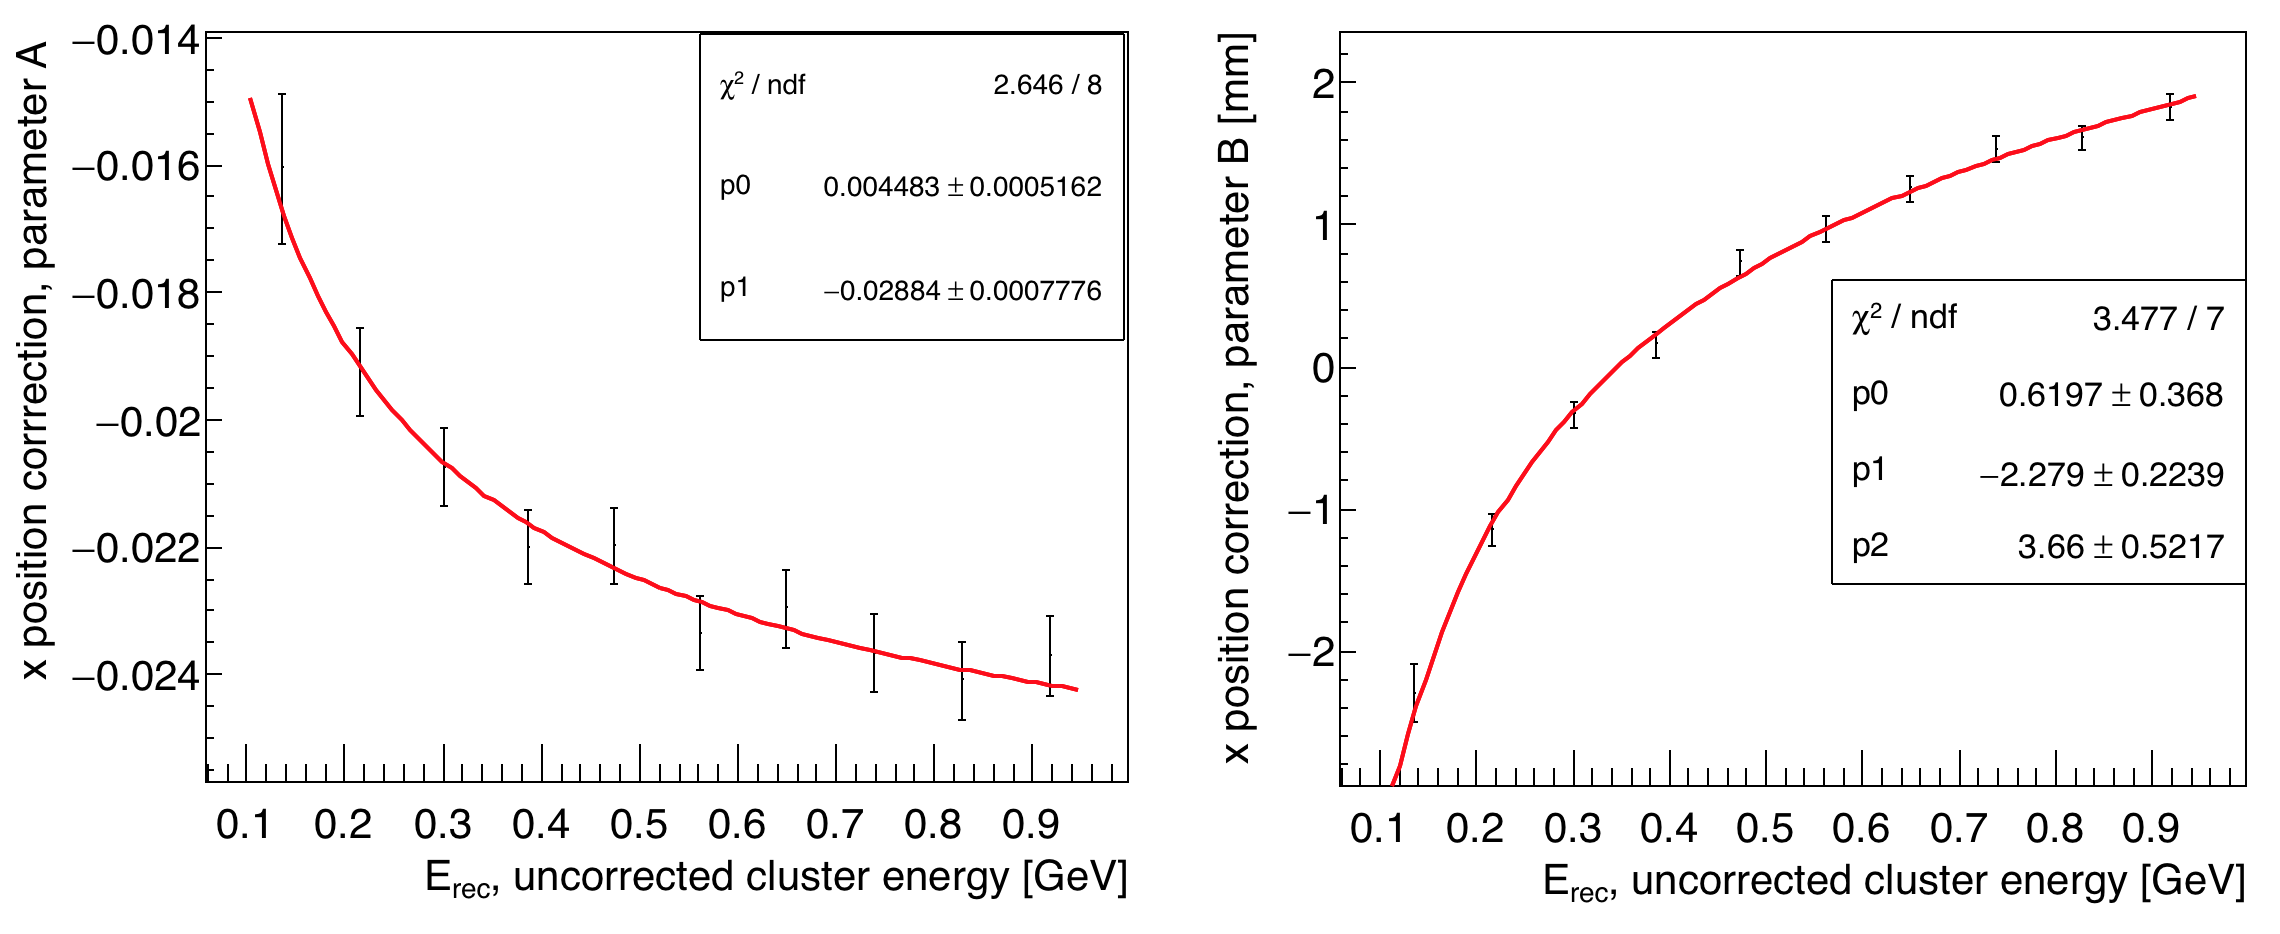
\includegraphics[width=1.0\textwidth]{pics/performance/xposcorrPar.png}
  \caption[Horizontal position correction dependence for electrons]{The horizontal position correction parameters of Equation~\eqref{eq:posncorr} as functions of the reconstructed cluster energy (without any further energy corrections for shower loss).}
  \label{Figure:xposcorrPar}
\end{figure}

The parameters in Figure~\ref{Figure:xposcorrPar} are fit to functions of the form:
\begin{equation}
\label{eq:posnCpar}
\begin{split}
A(E_{rec}) & =  \dfrac{p0}{\sqrt{E_{rec}}}+p1\\
B(E_{rec}) & =  p0\times E_{rec} +\dfrac{p1}{\sqrt{E_{rec}}}+p2
\end{split}
\end{equation}
The correction values for all three particle types are summarized in Table~\ref{tab:horizPosCorr}. Position corrections are not needed for the vertical cluster position.

\begin{table}[htb]
\caption{Horizontal position corrections.}
\label{tab:horizPosCorr}
\centering
\begin{tabular}{|c|c|c|}
\toprule
%\multicolumn{2}{c}{Name} \\
%\cmidrule(r){1-2}
Particle & $A(E_{rec})$ & $B(E_{rec})$ \\
\midrule
electron & $0.004483/\sqrt{E_{rec}}-0.02884$ & $0.6197E_{rec}-2.279/\sqrt{E_{rec}}+3.66$ \\
positron & $0.006887/\sqrt{E_{rec}}-0.03207$ & $-0.8048E_{rec}+0.9366/\sqrt{E_{rec}}+2.628$ \\
photon & $0.005385/\sqrt{E_{rec}}-0.03562$ & $-0.1948E_{rec}-0.7991/\sqrt{E_{rec}}+3.797$ \\
\bottomrule
\end{tabular}
\end{table}


\subsubsection{Position resolution}

After applying the position corrections to each particle-type at the simulated energies, the residual between the measured and simulated position reconstruction is obtained. The fitted residuals for the position of 1~GeV electron clusters are shown in Figure~\ref{Figure:corrPosnsFits}.
\begin{figure}[htb]
  \centering
      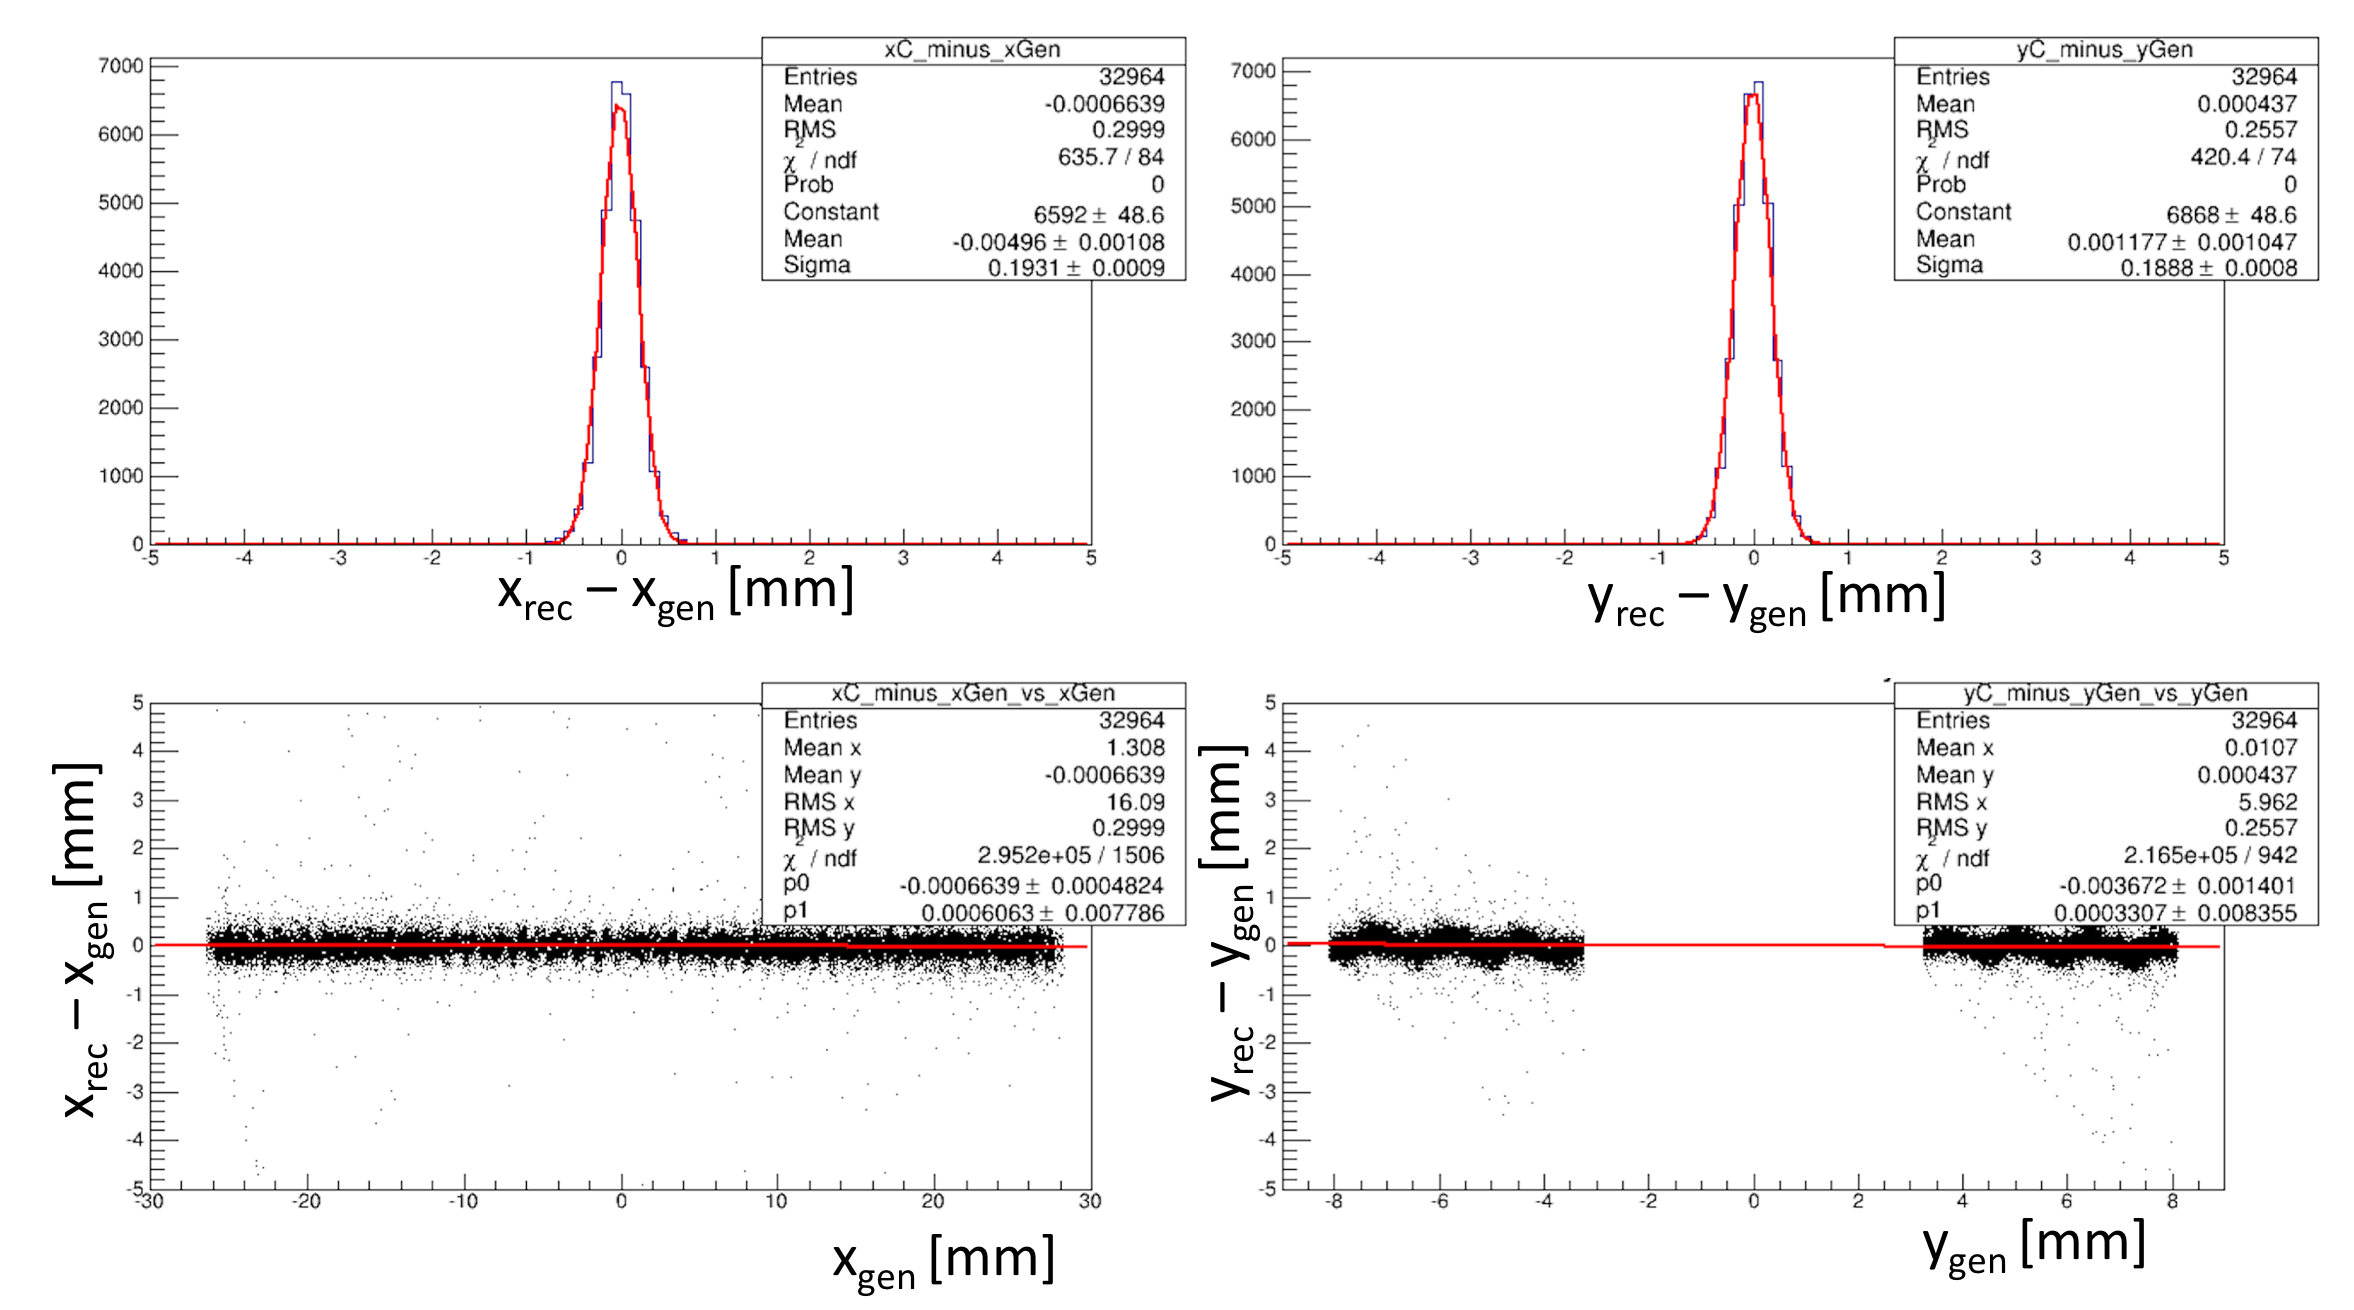
\includegraphics[width=1.0\textwidth]{pics/performance/corrPosnsFits.png}
  \caption[Position resolution for 1~GeV electrons]{The position resolution for 1~GeV electrons, after applying the horizontal position corrections.}
  \label{Figure:corrPosnsFits}
\end{figure}
As shown in Figure~\ref{Figure:corrPosnsFits}, no correction is required when reconstructing the vertical position of the cluster. The energy-dependent resolution of both the horizontal and vertical position of reconstructed clusters can be seen for electrons in Figure~\ref{Figure:emPosnResn}. 
\begin{figure}[htb]
  \centering
      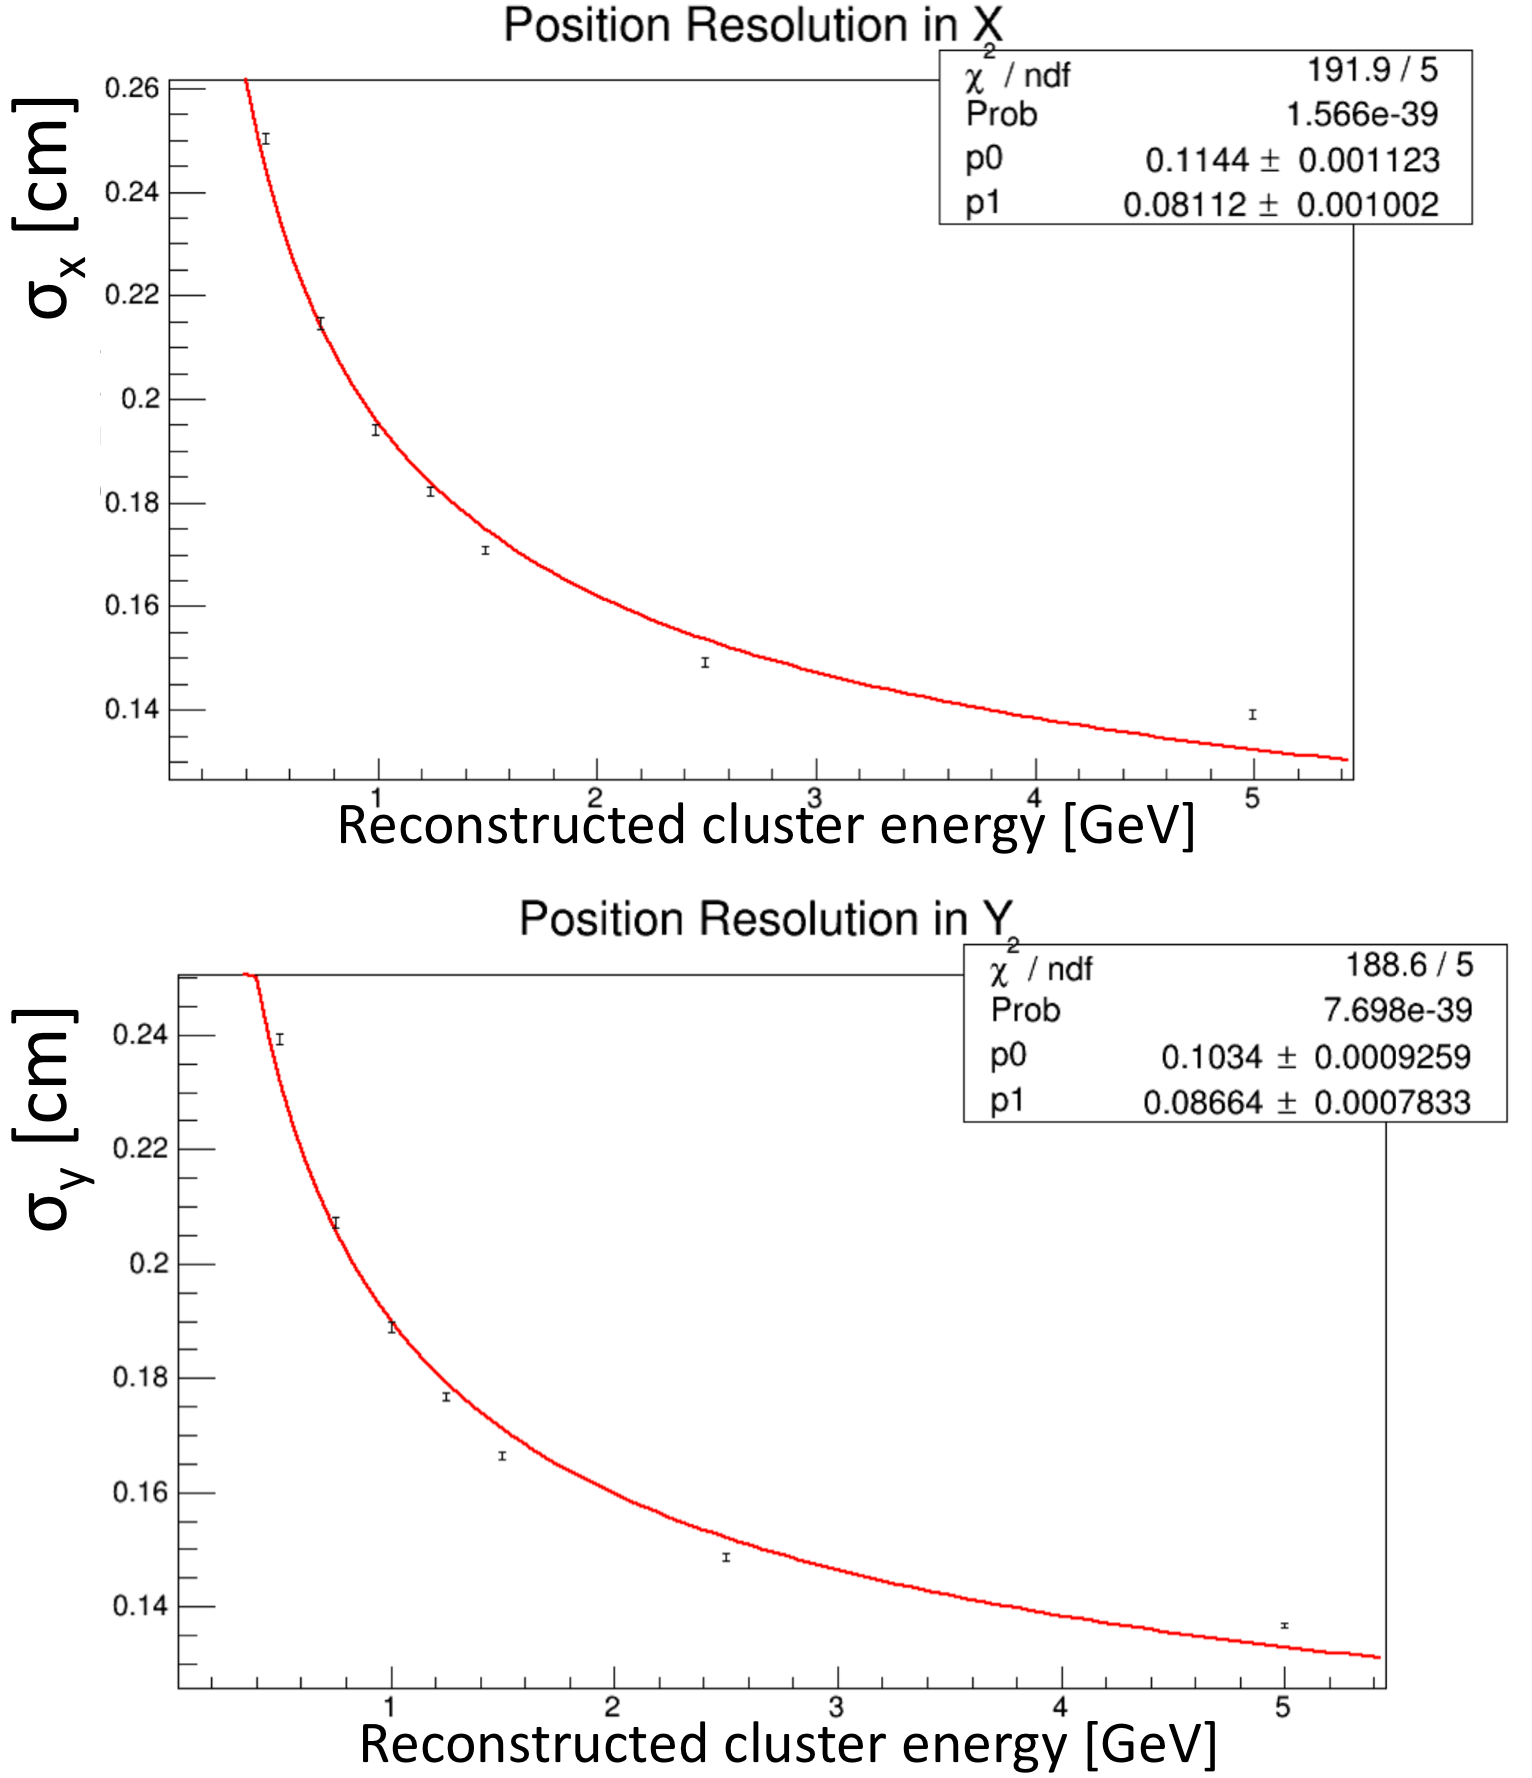
\includegraphics[width=0.7\textwidth]{pics/performance/emPosnResn.png}
  \caption[Energy-dependent position resolution for electrons]{The energy-dependence of the position resolution for electrons as determined from simulation.}
  \label{Figure:emPosnResn}
\end{figure}
The position resolution is parameterized as:
 
\begin{equation}
\label{eq:posnRes}
\begin{split}
\sigma_x \textrm{[cm]}& =  \dfrac{p0_x}{\sqrt{E}}+p1_x\\
\sigma_y \textrm{[cm]}& =  \dfrac{p0_y}{\sqrt{E}}+p1_y
\end{split}
\end{equation}
where the parameters $p0$ and $p1$ are fit to the position resolution as a function of energy. The position resolution is better than 2~mm for 1~GeV electrons. As the ECal face is located at  approximately 1.4~m from the target, the ECal provides valuable position information when matched with a track. The ECal position resolution functions for all particle types is given in Table~\ref{tab:PosnResTable}. The reconstructed cluster energy ($E_{rec}$ in units of GeV) is not corrected for shower-loss effects. 

\begin{table}[htb]
\caption{Position resolution.}
\label{tab:PosnResTable}
\centering
\begin{tabular}{|c|c|c|}
\toprule
%\multicolumn{2}{c}{Name} \\
%\cmidrule(r){1-2}
Particle & $\sigma_x$ [mm] & $\sigma_y$ [mm] \\
\midrule
electron & $0.1144/\sqrt{E_{rec}}+0.08112$ & $0.1034/\sqrt{E_{rec}}+0.08664$ \\
positron & $0.1268/\sqrt{E_{rec}}+0.07711$ & $0.1068/\sqrt{E_{rec}}+0.08423$ \\
photon & $0.1255/\sqrt{E_{rec}}+0.08877$ & $0.1005/\sqrt{E_{rec}}+0.08867$ \\
\bottomrule
\end{tabular}
\end{table}
\subsection{Energy Calibration using cosmic rays}
\begin{figure}[htb]
  \centering
      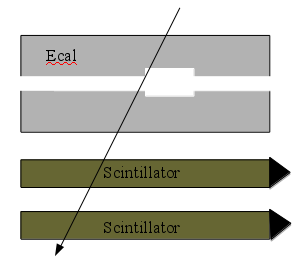
\includegraphics[width=0.7\textwidth]{pics/performance/cosmicschematic.png}
  \caption[Setup for ECal cosmic ray calibration]{Experimental setup for the cosmic ray calibration. The event read out was triggered by the coincidence of the two scintillators.}
  \label{Figure:cosmicScheme}
\end{figure}
The large area APDs enabled the ECal to have the sensitivity to detect signals from cosmic muons traversing the ECal crystals perpendicularly. This signal was used for the initial calibration of the modules. The experimental setup for the cosmic calibrations used two scintillators placed below the ECal to trigger readout of all of the crystals. A schematic for the setup of the cosmic calibration is shown in Figure~\ref{Figure:cosmicScheme}. Each scintillator measures 75~cm long, 22~cm wide and 5~cm thick, covering a slightly larger perpendicular area than the ECal crystals. The two scintillators are less than half a meter apart with the closest scintillator less than half a meter beneath the ECal. \\
\indent The rates and energy deposited in the crystals from cosmic ray muons was studied using Monte Carlo simulation. The energy deposited in each crystal in a layer is proportional to the path length of the track passing through the crystal. From simulation, the average energy deposited in a crystal by a cosmic ray passing vertically though the ECal is shown in Figure~\ref{Figure:cosmicEdep}  (i.e., only tracks passing through one crystal in each row were included).

\begin{figure}[htb]
  \centering
      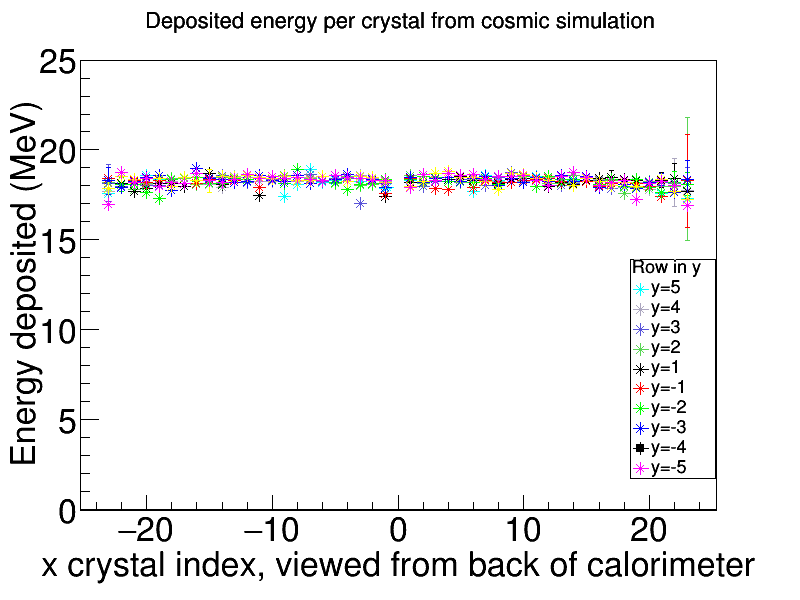
\includegraphics[width=0.8\textwidth]{pics/performance/cosmicEdep.png}
  \caption[Simulation of energy deposited per ECal module from cosmic rays]{The simulated cosmic ray muon energy deposition per crystal of the ECal. The mean energy was 18.3~MeV.}
  \label{Figure:cosmicEdep}
\end{figure}
Additionally, the cosmic ray muon track had to pass through the crystals immediately above and below the struck crystal. For crystals near edges, the geometrical requirement was adjusted to include the two crystals immediately above (or below for cases where the edge is above the crystal) the crystal being read out. The average energy deposited per crystal is approximately 18.3~MeV~\cite{Agashe:2014kda}. In data, the raw FADC waveform for each crystal is read out, and the event is kept for further study after applying strict coincidence cuts between the two scintillators. The trigger rate for data is about 7~Hz. 30$\%$ of events passed the coincidence cut between the scintillators. For a track passing vertically through all ten ECal layers, we can see the signal in each crystal as shown in Figure~\ref{Figure:cosmicSig}.

\begin{figure}[htb]
  \centering
      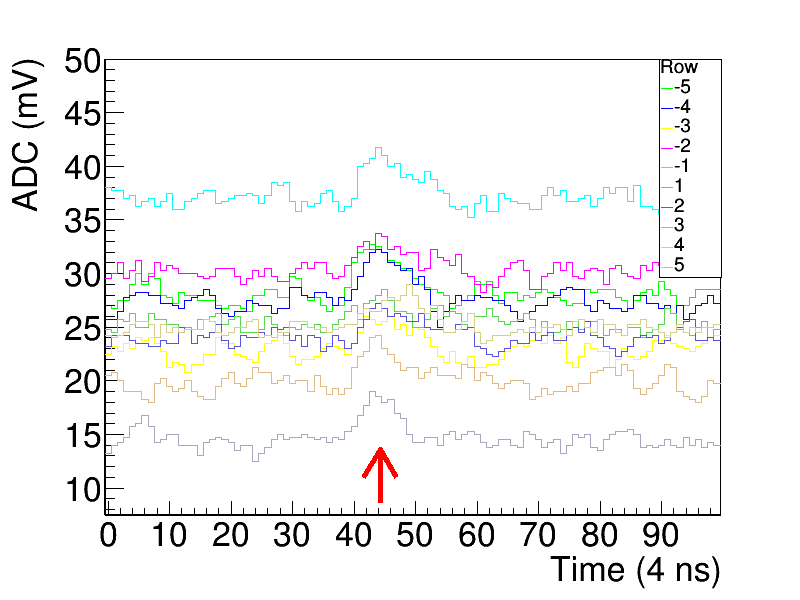
\includegraphics[width=0.7\textwidth]{pics/performance/cosmicSignal.png}
  \caption[Real cosmic ray signal in raw FADC waveform passing vertically through ECal]{The crystal signals plotted versus time for a cosmic ray signal passing vertically through all ten layers of crystals in the ECal. Each crystal's signal is separated vertically in this plot by its pedestal. The arrow indicates the approximate time that the cosmic signal passed through the detector. 1~V corresponds to 4096 FADC channels.}
  \label{Figure:cosmicSig}
\end{figure}

As seen in Figure~\ref{Figure:cosmicSig}, each FADC channel has a different pedestal value. The pedestal for each event was calculated as an average of twenty bins toward the beginning of the time window. By searching for a threshold crossing in the time window where cosmic events occurred, the signal was then fully integrated and the pedestal was subtracted\footnote{The raw waveform thresholds were 2.5~mV in 2015 and increased to 3.5~mV in 2016 to accommodate the larger signals after the removal of the splitters. As shown in Figure~\ref{Figure:readoutChain}, the $1/3$ of the signal from the ECal was split to go to the TDC modules. The splitters and TDCs were removed for the 2016 engineering run so that the full signal could be measured by the FADC.}. Geometric cuts are then applied to the data in offline analysis. Crystals having peaks over a certain threshold must have at least an adjacent crystal located both above and below with a threshold crossing, but the signals in the crystals to the left and right must not cross threshold. These cuts ensure that the track passed as vertically as possible through the ECal (reducing the variation in path length through each crystal). A fit to the energy spectrum in a single crystal is shown in Figure~\ref{Figure:cosmicFit}.\\
\begin{figure}[htb]
  \centering
      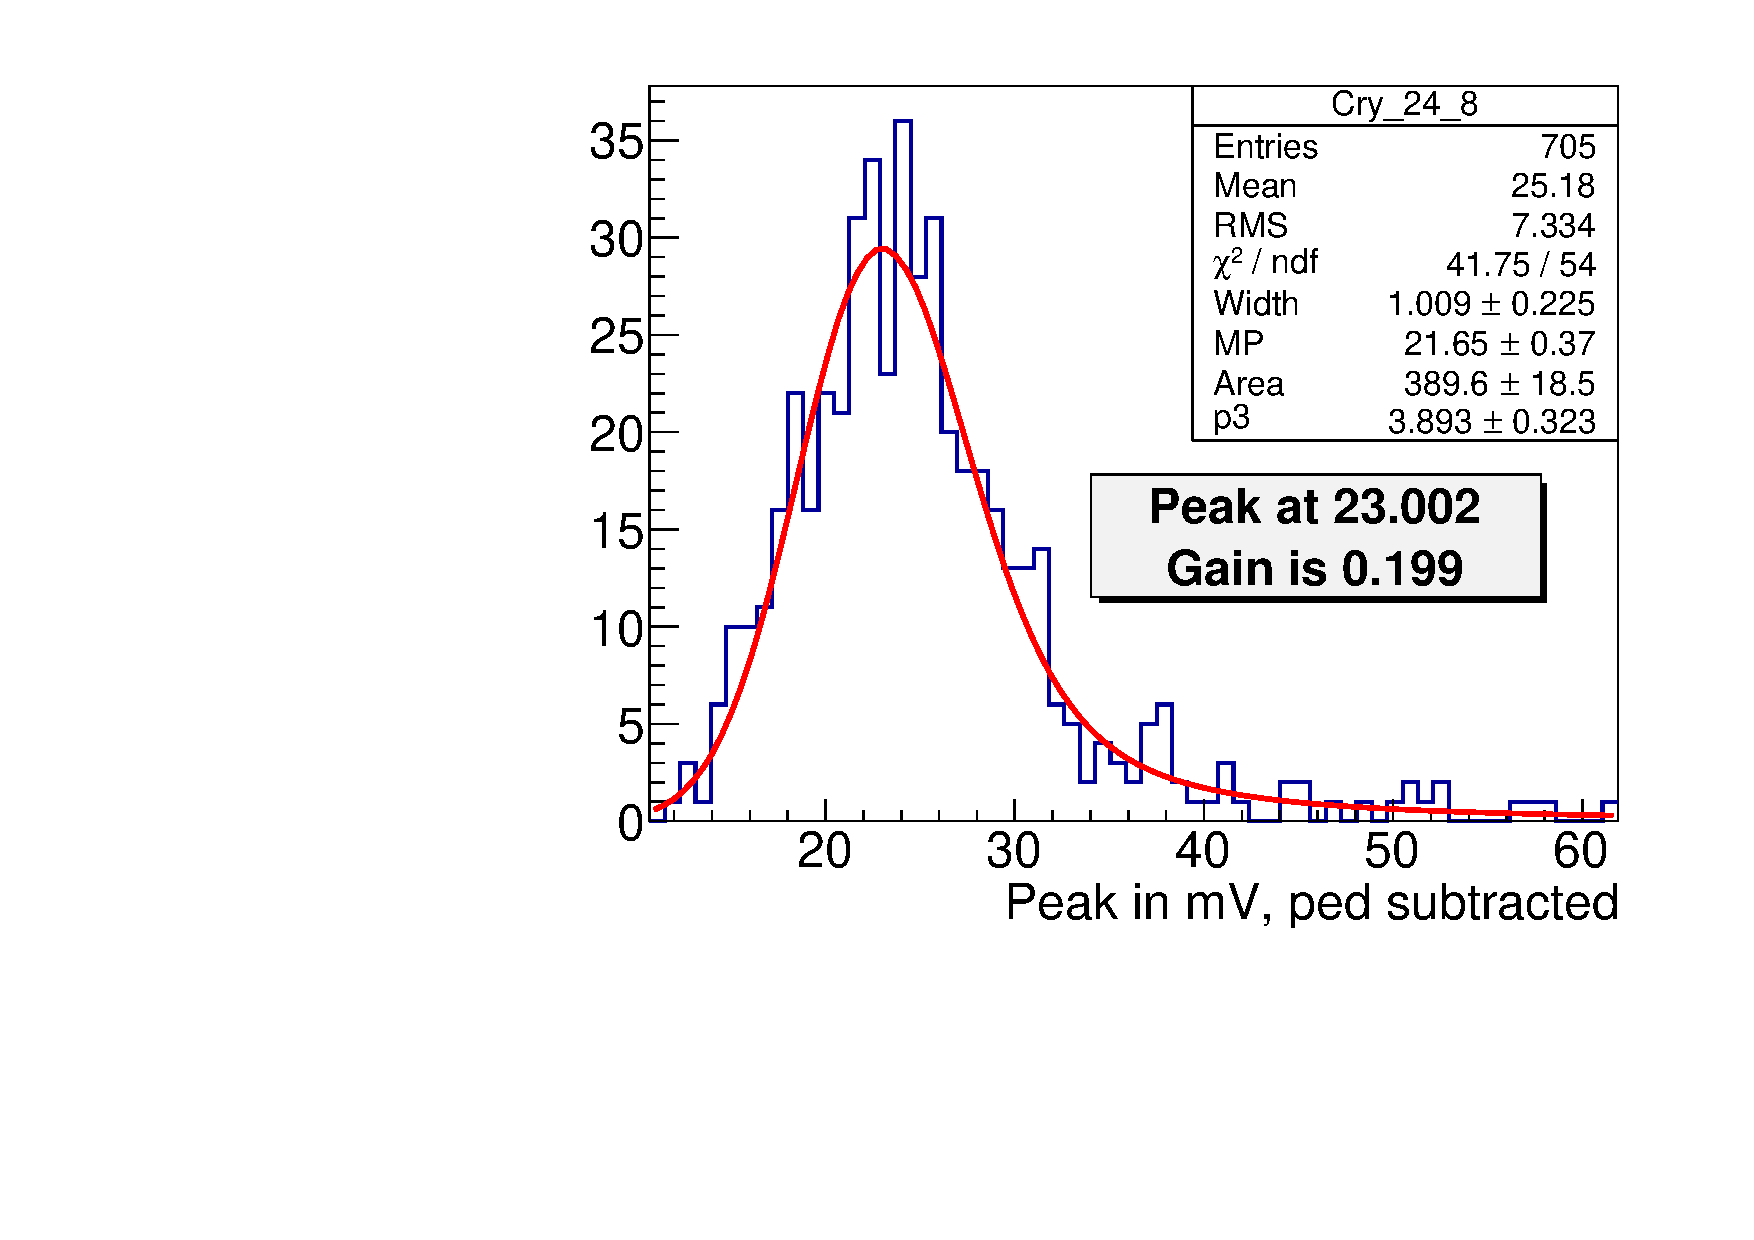
\includegraphics[width=0.8\textwidth]{pics/performance/cosmicFitExample2015.pdf}
  \caption[Integrated cosmic signal in ECal fitted for calibration]{A histogram of the energy (signal pulse integral) deposited by cosmic ray signals in a single crystal. The fit used a Landau-Gaussian convolution function. The peak location was calculated numerically from this fit.}
  \label{Figure:cosmicFit}
\end{figure}
The fit shown in Figure~\ref{Figure:cosmicFit} utilized a Landau-Gaussian convolution as the Landau part corresponds to the crystal's response to a particle's energy deposition, and the Gaussian part accounts for the statistical nature of the electronics shaping and readout. The peak of the fit is calculated numerically, and the initial conversion from pulse-height to energy (MeV) is obtained (called the Gain factor). The gain factor is calculated using the measured peak position in units of FADC pulse-integral and the known energy deposited from the simulation in units of MeV:
%1~V corresponds to 4096~FADC channels. The 4096~FADC counts can be set to 1~V or 2~V, but for 2015 and 2016 running, the setting was 1~V. 
\begin{equation}
	\label{eq:gain}
	\textrm{Gain} = \dfrac{\textrm{[MeV]}}{\textrm{[FADC pulse-integral]}} 
\end{equation}
The full ECal was calibrated with about 60~hours of cosmic ray data. The resultant gains for all channels in the 2015 engineering run are shown in Figures~\ref{Figure:cosmicG} and~\ref{Figure:cosmicGhisto}.

\begin{figure}[htb]
  \centering
      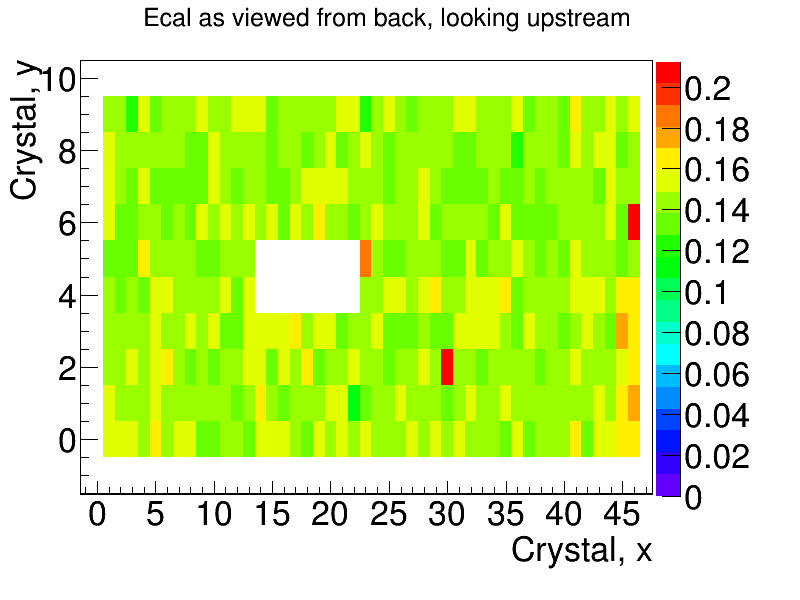
\includegraphics[width=0.7\textwidth]{pics/performance/cosmicGains2015.png}
  \caption[Resulting 2015 gain calibration in the ECal using cosmic ray muons shown by ECal module position]{Resulting gain calibration for each crystal using cosmics for the 2015 engineering run where the $z-$axis color is shown in units of [MeV/FADC pulse-integral].}
  \label{Figure:cosmicG}
\end{figure}


\begin{figure}[htb]
  \centering
      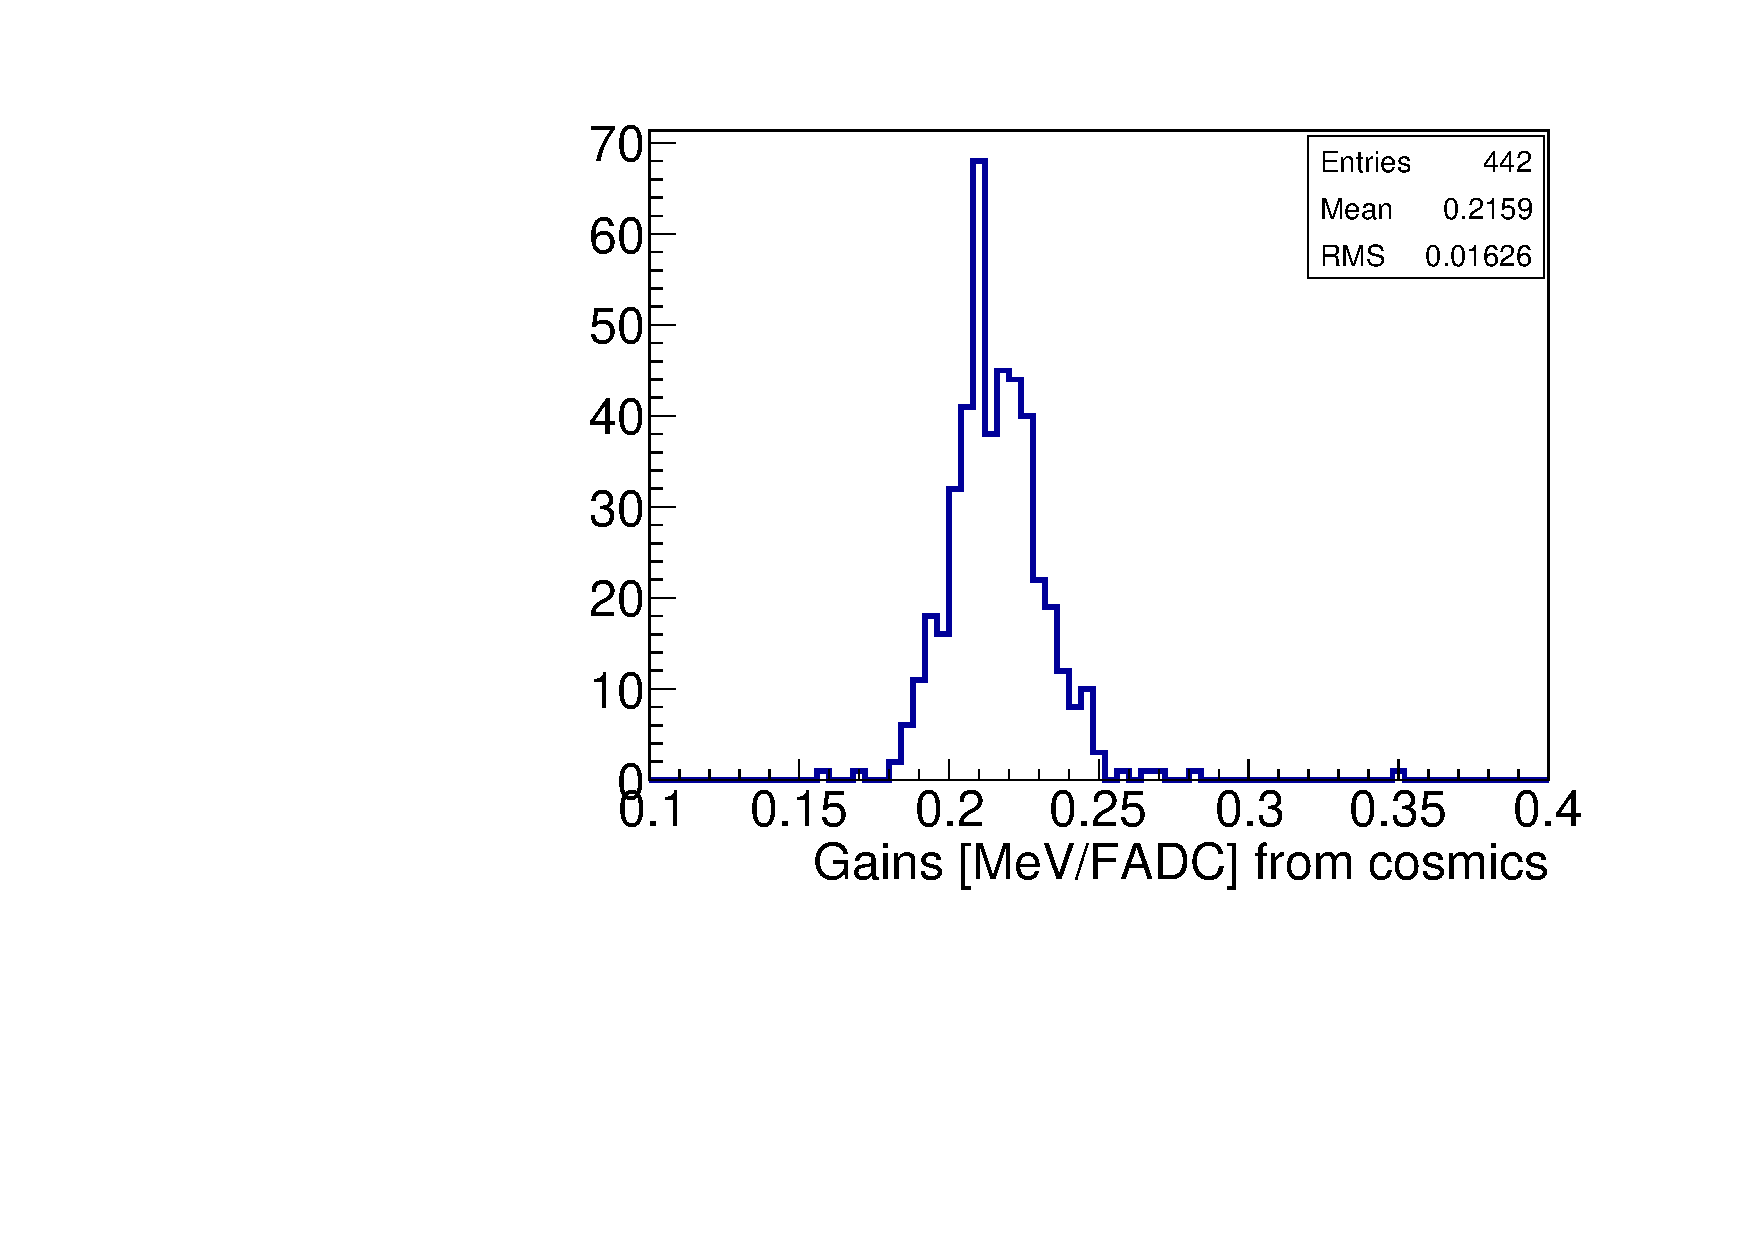
\includegraphics[width=0.7\textwidth]{pics/performance/cosmicGainsMay15.pdf}
  \caption[Distribution of the resulting 2015 gains in the ECal using cosmic ray muons]{Resulting gain calibration for all crystals using cosmics for the 2015 engineering run.}
  \label{Figure:cosmicGhisto}
\end{figure}

With the splitters installed in the ECal readout chain (shown in Figure~\ref{Figure:readoutChain}), the average gain value was around 0.2~MeV/FADC pulse-integral for the 2015 engineering run. After the removal of the splitters in January 2016, prior to the spring run, the average gains were found to be around 0.13~MeV/FADC pulse-integral.

\subsection{Ecal signal pulse fitting} \label{pulsefitting}
All data was taken using the FADC250 modules which sample at 250~MHz, or every 4~ns. While the firmware has various modes for recording data, data size was not an issue and Mode 1 was used during both engineering runs. Mode 1 preserves the full measured waveform for a module hit to allow for improved methods for extracting the energy and time information in offline analysis. The trigger decision to read out a module is based off a leading edge threshold which was set to 12~FADC pulse-height units in the 2015 engineering run. \\
\indent The full response for each module was carefully studied in order to understand the time response and shaping effects of the preamplifier on the ECal modules \cite{charles_2014}. The raw waveform response was best described by the sum of the pedestal $P$ and a $3$--pole function for the pulse with width $\tau$ occurring at time $t_0$:

\begin{equation}
	\label{eq:thrpole}
	E(t) = P + \dfrac{A}{2\tau^3}(t-t_0)^2e^{-(t-t_0)/\tau} 
\end{equation}
where the pulse integral value is the parameter $A$. When $t<t_0$, the pulse amplitude is zero. The best resolutions were found by fixing the width parameter for each module as the average measured over several pulses. An example fit is shown in Figure~\ref{Figure:mode1fit}.

\begin{figure}[htb]
  \centering
      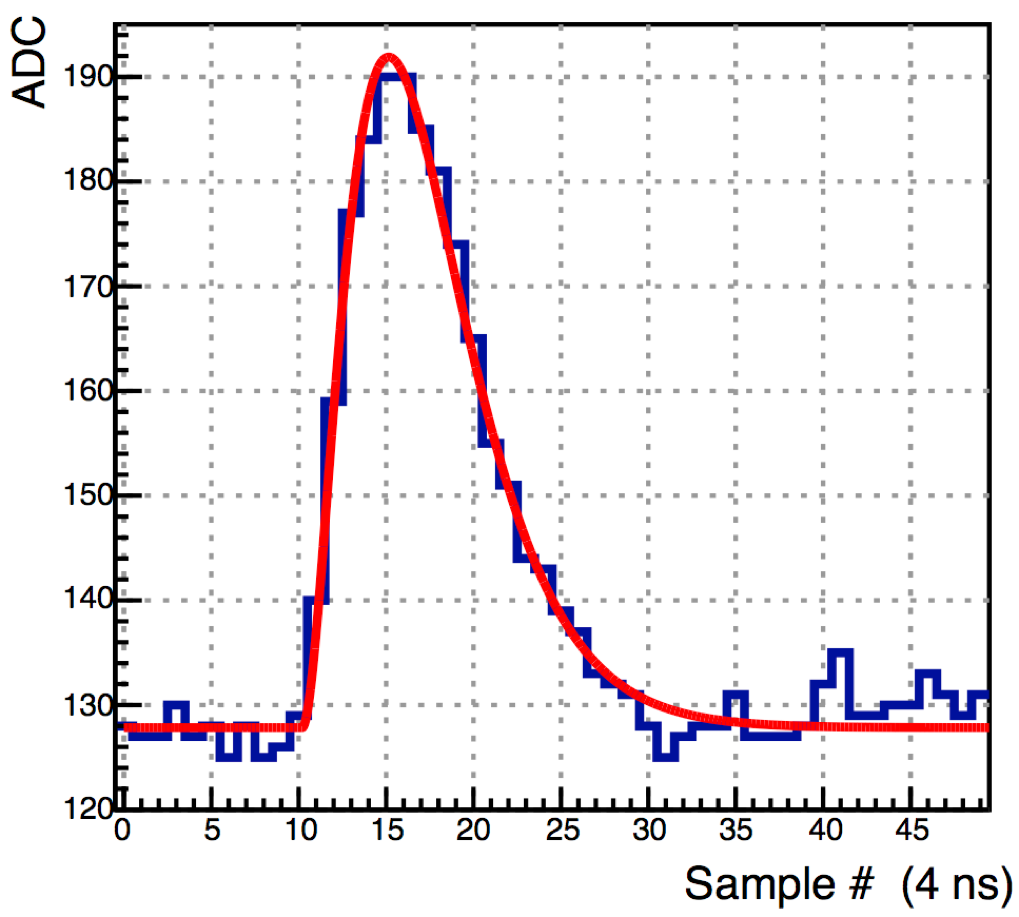
\includegraphics[width=0.5\textwidth]{pics/performance/mode1fit.png}
  \caption[Pulse-fitting to Mode 1 ECal data]{Example fit to a real ECal module pulse.}
  \label{Figure:mode1fit}
\end{figure}

The pedestal is calculated event-by-event and initialized by a running average over the previous fits for the pulse. The fit range was set to 20~ns before and 60~ns after the threshold crossing in order to eliminate contamination from pile-up signals in the same event~\cite{baltzell_ecal_2015}. The offline pulse-fitting of the raw waveform demonstrated the best time resolution and energy resolution when compared to the other hardware integral methods that could have been implemented~\cite{baltzell_ecal_2015}.

\subsection{Calibration using elastically-scattered electrons}
The calibration using cosmic ray muons was sufficient for initial data-taking with the electron beam, but the overall energy calibration of the ECal is optimal at higher energies. The ECal detects elastically scattered electrons that peak, after correction for shower leakage effects, at the beam energy. As the target is off centerline beam right, there are geometric effects that prevent elastically-scattered beam energy electrons from illuminating the entire ECal~\cite{szumila-vance_hps_2016}. From simulation, the rightmost column of crystals, and the five leftmost columns of crystals cannot be calibrated using elastically-scattered electrons. \\
\indent To calibrate the ECal using elastically-scattered electrons, we selected events where the seed hit crystal carried at least 60$\%$ of the overall cluster energy. The seed hit was also required to have more than 450~MeV in the 2015 data (1.1~GeV for the 2016 data), to have triggered a Singles 1 event readout from the DAQ, and to have occurred in the optimal trigger timing window. The cluster energy was associated with the seed hit module for the calibration. The calibration uses an iterative procedure, by which the reconstructed cluster energy is matched to the expected simulated energy (prior to energy corrections). For each crystal's cluster energy, an iteration coefficient is found that reflects the ratio of the cluster energy measured in Monte Carlo to the cluster energy found for that iteration:\\
\begin{equation}
	\label{eq:feeiter}
	C_i = \dfrac{MC_{peak}}{data_{peak}}
\end{equation}
After each iteration, this ratio $C_i$ is applied to the to the original gain coefficient as well as any coefficient found from a previous iteration. The data is re-processed applying these changes to the gains and clustering is re-run. This procedure continues until the correction coefficients found in a particular iteration are all less than 1$\%$. Crystals on the edge of the acceptance with poorly resolved peaks were given an iteration coefficient of 1. After completion of the calibration (approximately 2-3 iterations)~\cite{szumila-vance_hps_2016}, the shower loss correction functions were applied to the reconstructed cluster energies. The measured ECal energy for elastically-scattered electron clusters in the fiducial region of the ECal is shown in Figure~\ref{Figure:FeeFidPeak}.
\begin{figure}[htb]
  \centering
      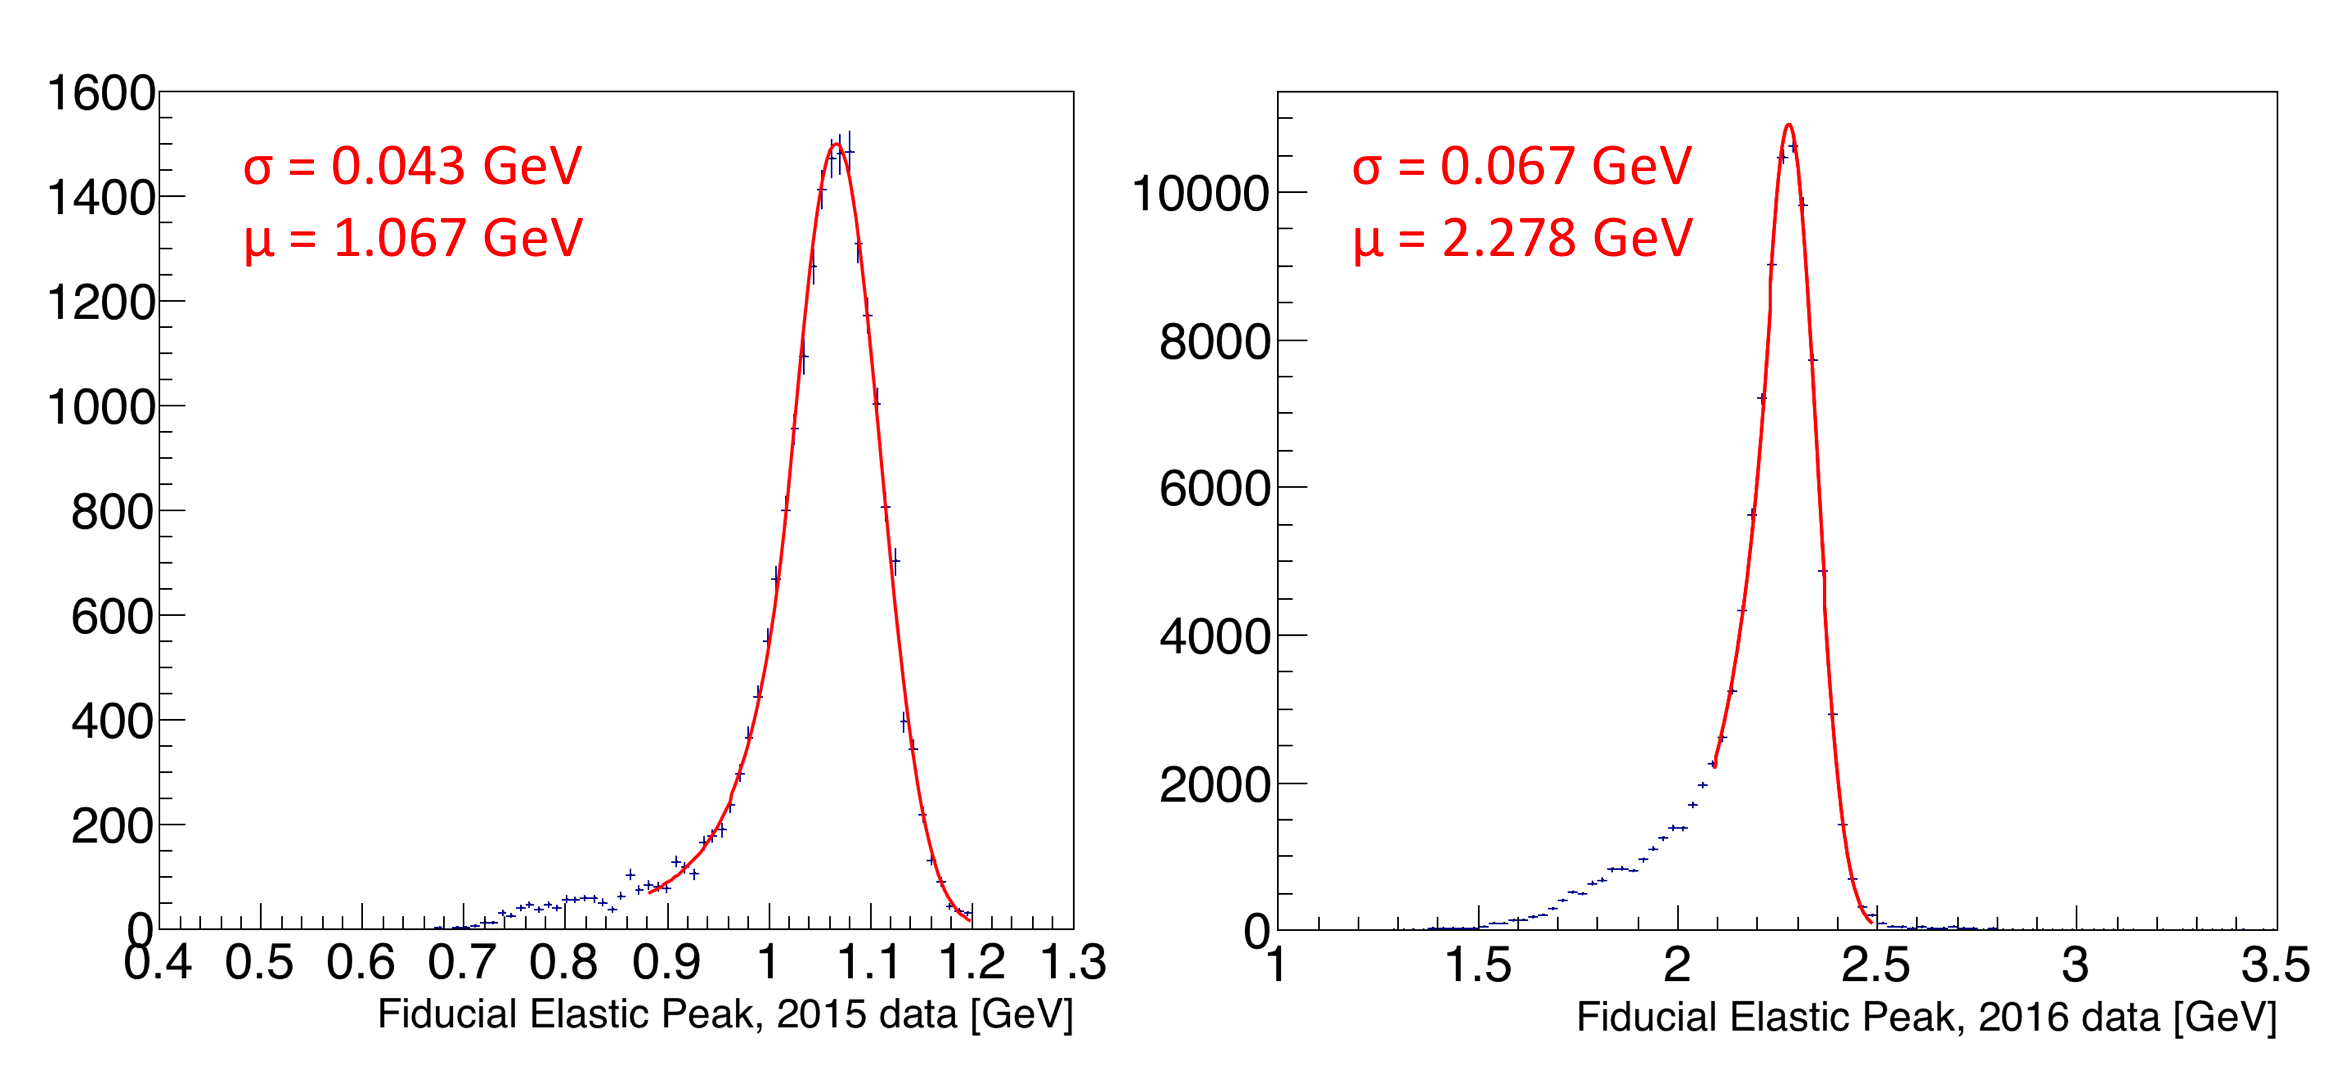
\includegraphics[width=0.9\textwidth]{pics/performance/feePeakFid.png}
  \caption[Reconstructed elastic peak in the ECal for the engineering runs]{The energy deposited in the fiducial region of the ECal for elastically-scattered electrons for the 2015 and 2016 runs is shown on the left and right, respectively. The peaks are fit with a Crystal Ball function and the peak position and widths are indicated. }
  \label{Figure:FeeFidPeak}
\end{figure}
The energy resolution improves with the beam energy. The cluster energy spectrum is fit with a Crystal Ball function which contains a Gaussian component and a power law low energy tail. The ECal has an energy resolution of approximately 4$\%$ in the fiducial region at 1~GeV and 2.9$\%$ at 2.3~GeV. \\
\indent The final gains obtained after calibration with elastically-scattered electrons were compared to the gains obtained with cosmics alone in order to check for systematic offsets. No systematic offsets were found. The comparison between the low and high energy calibrations tells us that cosmic calibration was roughly accurate, but it is limited in telling us anything about how linear the gain response is of the ECal between these two points in energy~\cite{szumila-vance_hps_2016}. Because not all of the crystals are calibrated using elastically-scattered electrons due to acceptance, the gains from cosmics were compared to the gains obtained from elastically-scattered electrons to check that there is no systematic offset. Any systematic difference would need to be applied to the crystals calibrated only with cosmics and the effects on the triggered data would need to be quantified. No systematic offset was observed. 
%\begin{figure}[H]
 % \centering
    %  \includegraphics[width=0.9\textwidth]{pics/performance/cosmicComp.png}
 % \caption[Gain comparison between cosmic and elastic calibration]{A comparison between the gains from he cosmic and elastic calibration is shown. Any overall systematic shift would need to be applied to crystals outside of the elastic calibration acceptance. }
%  \label{Figure:cosmicComp}
%\end{figure}

\subsection{Wide angle bremsstrahlung for studies of edge effects}
The primary physics trigger looks for events with two clusters. However, it also recorded a high yield of WAB events composed of an electron and a photon. The spectrum of cluster energies in the 2015 engineering run data set shows an excess of WAB events occurring where the energy sum of the two particles is approximately equal to the beam energy. \\
\indent Initial studies showed that the energy sum of two particles in WAB events having mid-range energies was lower than the reconstructed elastic energy, indicating that the shower loss corrections in the mid-range beam energy required further investigation. WAB events were used to refine the shower loss corrections for mid-range energy particles. WAB events are identified by having one track-matched cluster and one cluster with no matching track. The reconstructed energy sum of of the two particles must equal the beam energy~\cite{szumila-vance_hps_2016}:
\begin{equation}
	\label{eq:wabBeam}
	E_i = \dfrac{E_{e^-}}{f_{e^-}(E_{e^-})}+\dfrac{E_{\gamma}}{f_{\gamma}(E_{\gamma})}
\end{equation}
where $f$ refers to the shower loss correction described by Equation~\eqref{eq:eclsf}. The underlying assumption is that the relationship between the electron and photon shower loss corrections found in Monte Carlo are preserved:
\begin{equation}
	\label{eq:wabRatio}
	 \dfrac{f_{e^-, data}(E_{e^-})}{f_{\gamma, data}(E_{\gamma})}= \dfrac{f_{e^-, MC}(E_{e^-})}{f_{\gamma, MC}(E_{\gamma})}
\end{equation}
In maintaining the relationships shown in Equations~\eqref{eq:wabBeam} and \eqref{eq:wabRatio}, a chi-squared minimization yields the optimal adjustments to the shower loss correction functions for mid-range energy particles:
\begin{equation}
	\label{eq:wabBeamChi}
	\chi^2 =\sum_{i} \dfrac{(E_{beam}-E_{sum})^2}{\sigma_{e^-}^2(E_{e^-})+\sigma_{\gamma}^2(E_{\gamma})}	
\end{equation}
For each event, the energy sum of the two corrected clusters, $E_{sum}$, is calculated as described by Equation~\eqref{eq:wabBeamChi}. The end result is a small correction to the shower loss correction functions that ranges across the cluster energies and never exceeds 2$\%$~\cite{szumila-vance_hps_2016}. After incorporating these updated corrections to the shower loss correction functions, the energy resolution can be extracted for all energies and positions in the ECal.  

\subsection{Energy resolution in data}\label{EcalResData}
The elastically-scattered electrons provided the cleanest point in extracting the energy resolution of the ECal at the beam energy. Using WAB particles, electrons and photons, the energy resolution of the ECal was characterized for energies less than the beam energy for different positions relative to the edges.\\
\indent To study the energy resolution in the fiducial region of the ECal, all electrons were matched to tracks, and the track position extrapolation to the face of the ECal was used to determine the electron's vertical distance relative to the beam gap edge. For WAB electrons, the photon cluster was required to be at least 10~mm from the ECal edges to avoid edge effects. By selecting WAB events where the energy difference between the two particles is less than 100~MeV, the resolution of the energy sum peak was fitted to extract the resolution. The resolution was extracted:
\begin{equation}
	\label{eq:eResExtract}
	\sigma_{E_{\gamma}+E_{e^-}}^2 = \sigma_{e^-}^2(E_{e^-})+\sigma_{\gamma}^2(E_{\gamma})
\end{equation}
When both particles are in the fiducial region and are roughly equal in energy, then the energy resolution of the sum could be divided by $\sqrt{2}$ assuming that the energy resolution of both particles is the same. This same procedure was used to study the resolution when the particle energies were more asymmetric in energy in order to obtain the single particle energy resolution at various energies. \\
\indent The experimentally-obtained fiducial energy resolution agrees well with Monte Carlo but is about 15$\%$ larger (see Figure~\ref{Figure:eResData}).
\begin{figure}[htb]
  \centering
      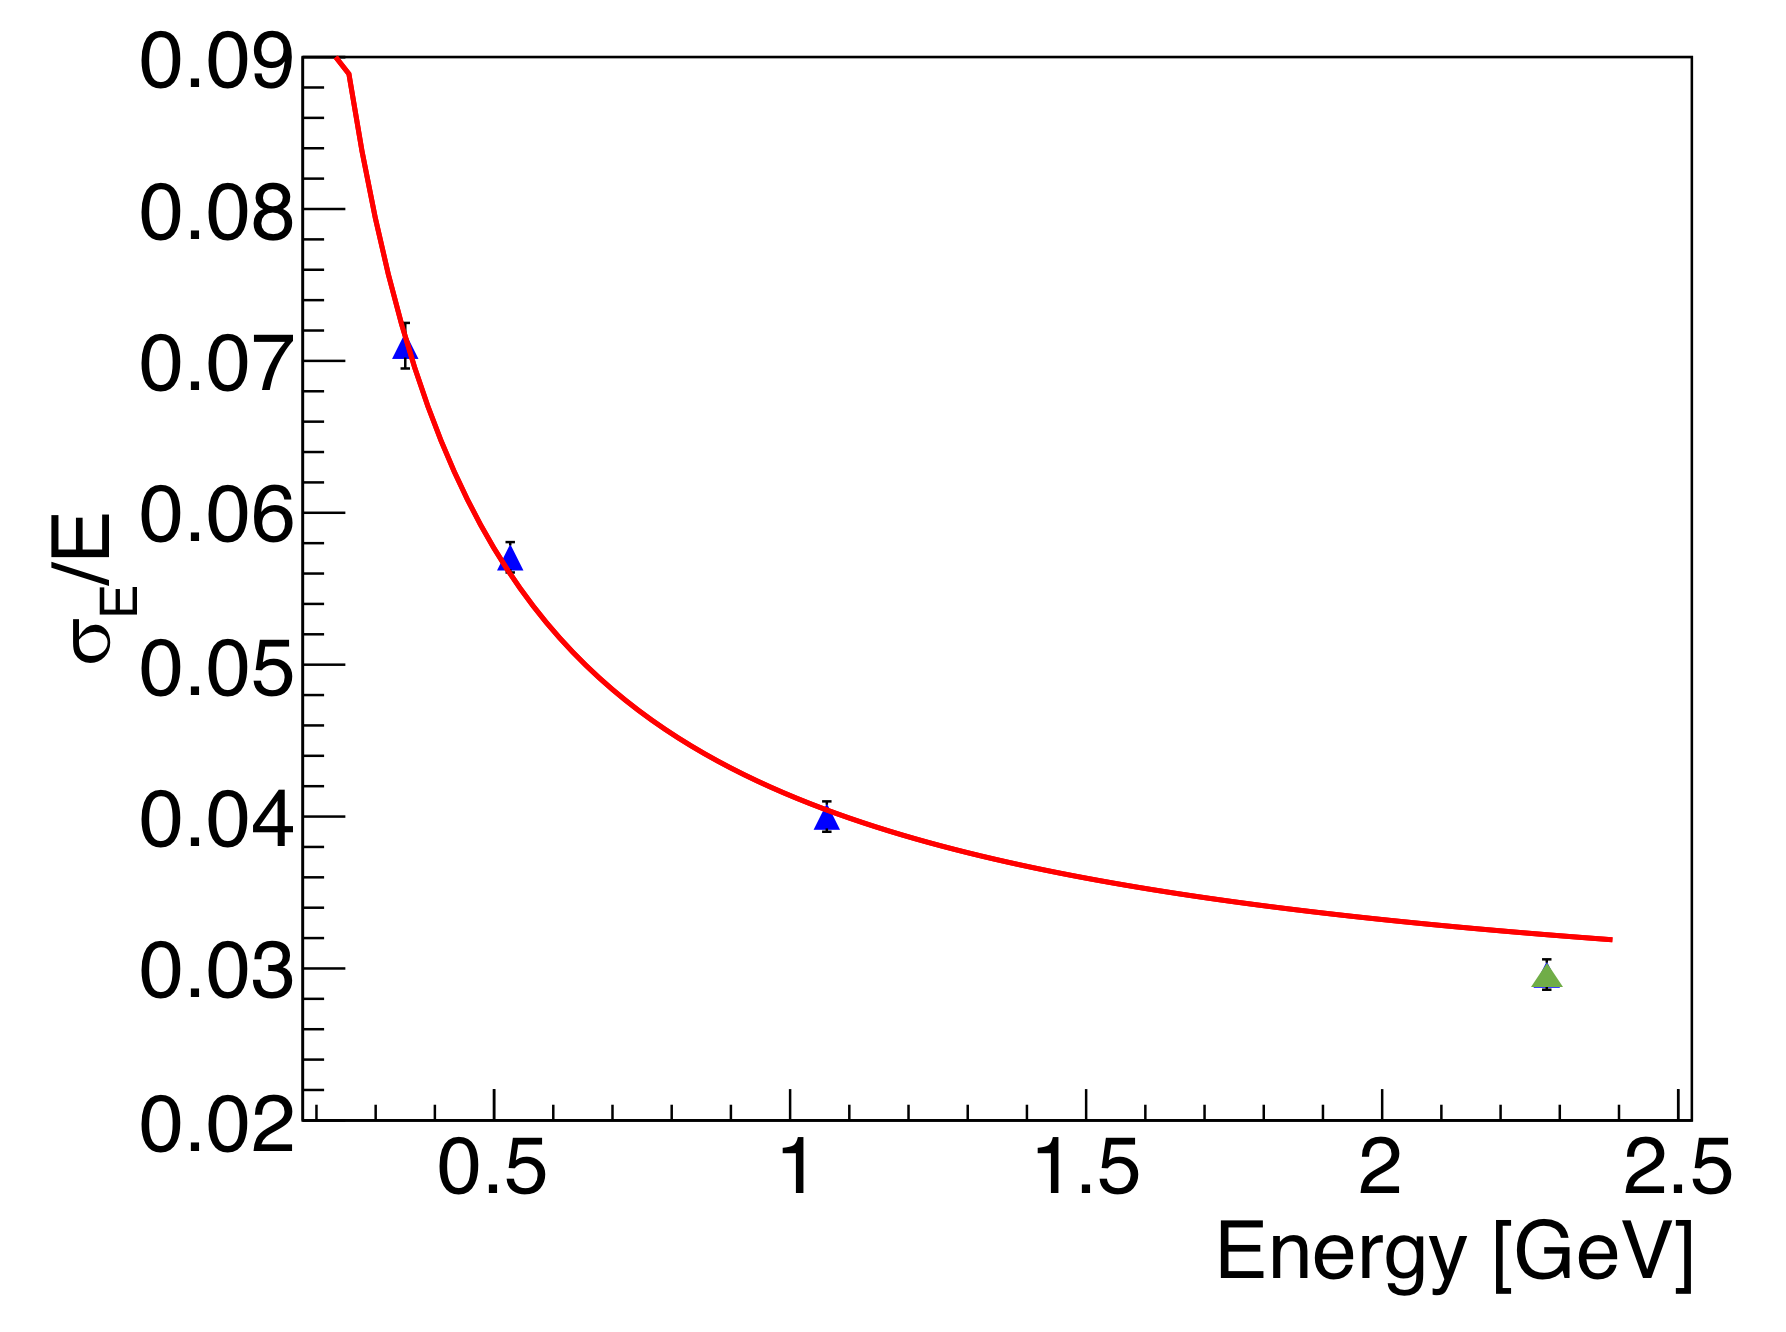
\includegraphics[width=0.6\textwidth]{pics/performance/eResData.png}
  \caption[Energy resolution of the ECal found in data]{The blue points are derived from the 2015 engineering run for the energy resolution of a single particle. The green point at approximately 2.3~GeV was determined from the elastic calibration of the 2016 engineering run data. The energy resolution was fit to the 2015 engineering run data only and extrapolated to higher energies.}
  \label{Figure:eResData}
\end{figure}
The fit to the energy resolution (energy in units of GeV) using the blue points from the 2015 engineering run data in Figure~\ref{Figure:eResData} is:\\
\begin{equation}
	\label{eq:eResData}
	\dfrac{\sigma_E}{E}(\%) = \dfrac{1.62}{E}\oplus\dfrac{2.87}{\sqrt{E}}\oplus2.5
\end{equation}
The first term is attributed to the noise from the pre-amplifiers and is roughly consistent to that found in Monte Carlo. The second term is related to the statistical fluctuations of the shower containment and the APD gain. This term is larger than the term found in Monte Carlo but is still consistent. The third term contains both the energy leakage out the back of the ECal as well as the crystal-to-crystal inter-calibration error. This term is significantly higher than anticipated from Monte Carlo, but is comparable to that found for the IC. It's possible that this term is affected by the inability to calibrate several crystals along the outer edges of the calorimeter with elastic electrons. \\
\indent The energy resolution from the 2.3~GeV engineering run (shown in green on Figure~\ref{Figure:eResData}) is slightly better than that predicted by the fit from the 1.056~GeV engineering run. It is likely that the energy resolution of the ECal improved because the signal going into the FADC modules was no longer split. \\
\indent The WAB events are a useful tool for studying the energy resolution in the ECal as a function of position relative to the edge. By selecting a photon cluster in the fiducial region of the ECal, the energy resolution of the electron (position given by the track projection at the ECal) could be measured at various energies. The second parameter of the energy resolution function described by Equation~\eqref{eq:eResData} (of the form $b/\sqrt{E}$) is strongly correlated with the vertical position relative to the beam gap edge. By fixing the other two terms to the values in the fiducial region, the value of the $b$ parameter was studied as a function of position~\cite{szumila-vance_hps_2016}. The final characterization of this value relative to the beam gap edge is shown in Figure~\ref{Figure:stochasticEdge}~\cite{balossino_hps_2016}.

\begin{figure}[htb]
  \centering
      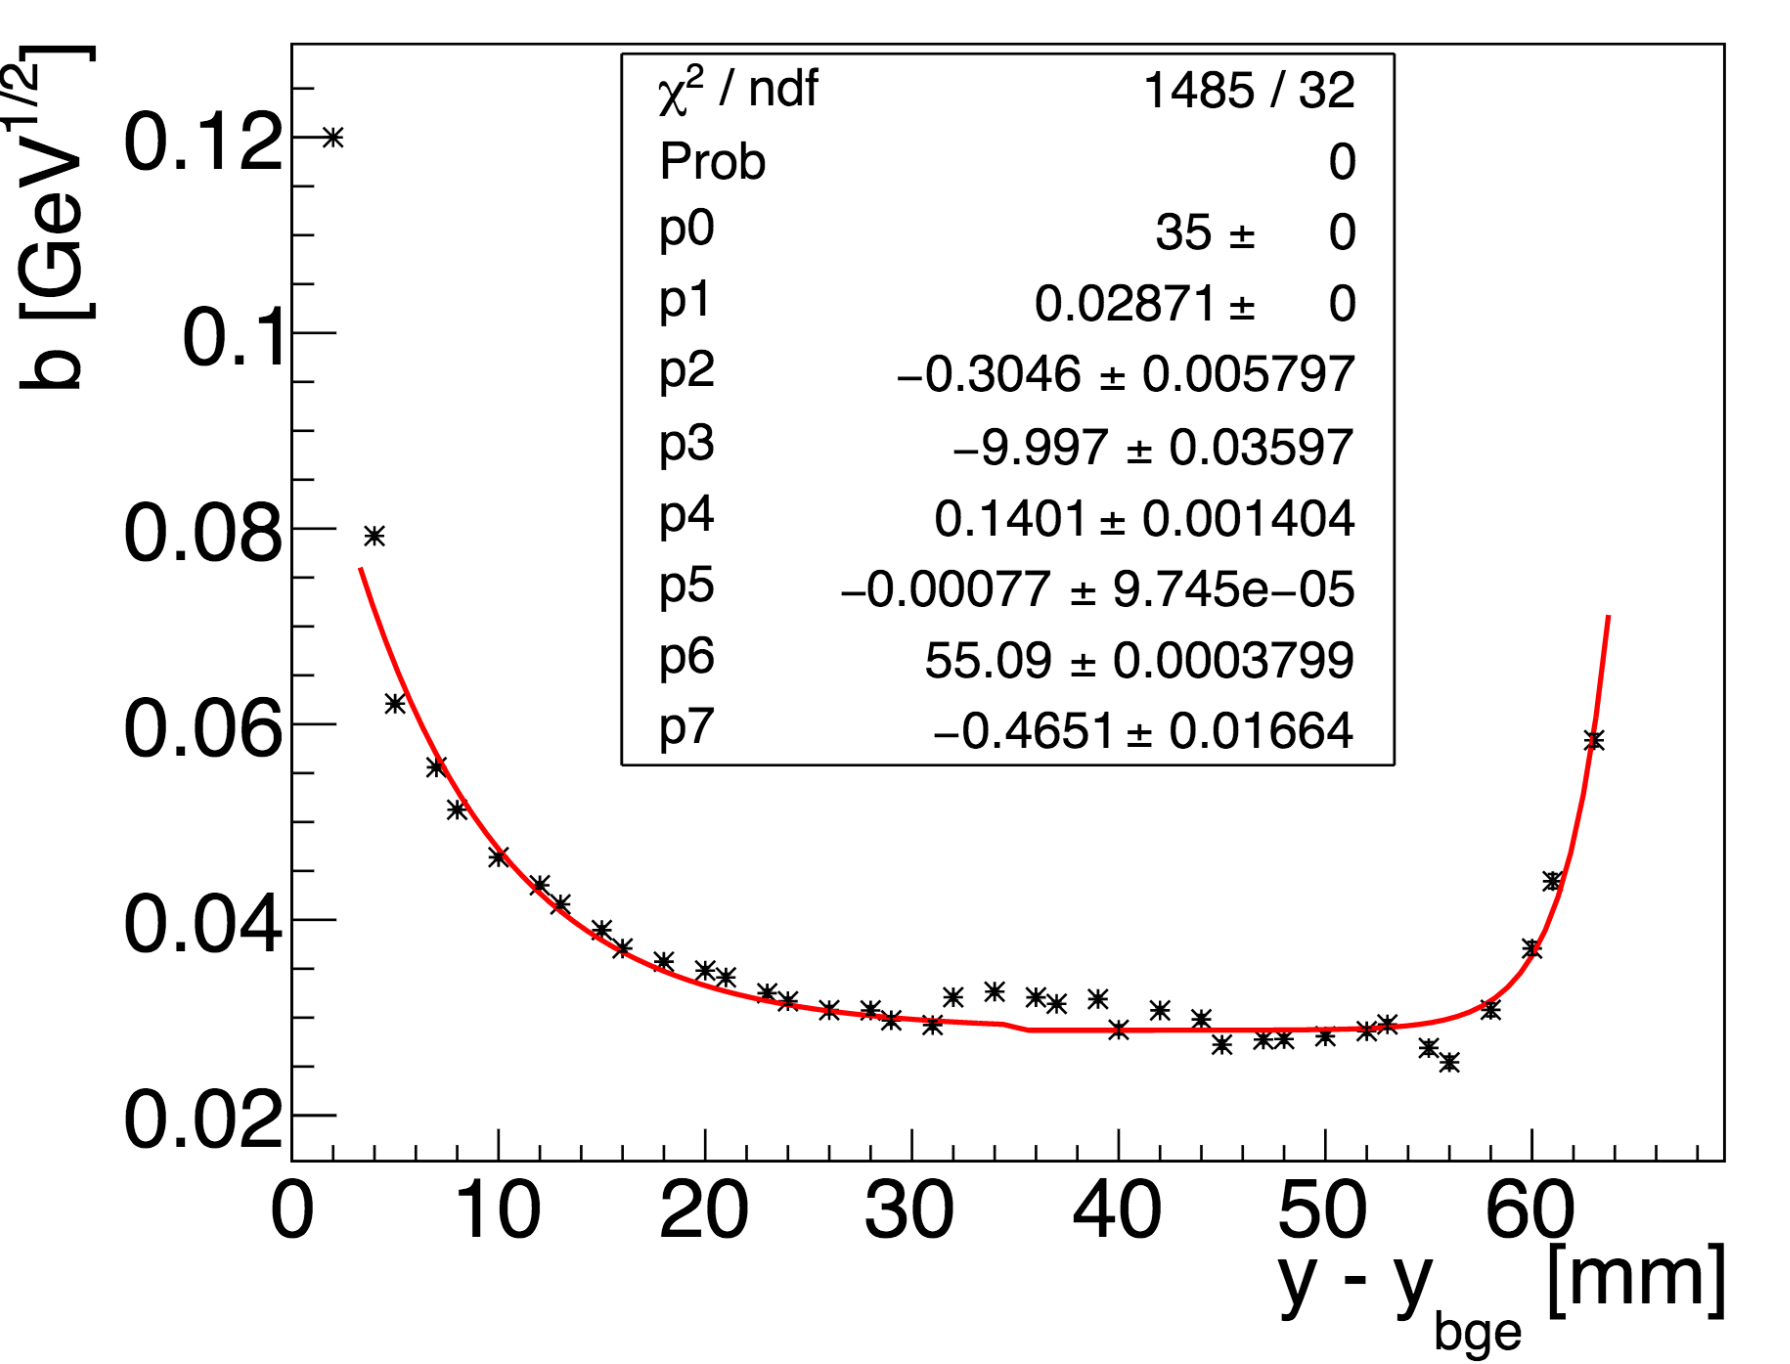
\includegraphics[width=0.5\textwidth]{pics/performance/eResEdgeEffect.png}
  \caption[Characterization of the energy resolution edge effects ]{The stochastic parameter $b$ (corresponding to the $1/\sqrt{E}$ term) of the energy resolution description is shown as a function of the vertical position relative to the ECal beam gap edge. The fit function is shown in Equation~\eqref{eq:finalRes}.}
  \label{Figure:stochasticEdge}
\end{figure}
The function that describes how the energy resolution varies with the position relative to the inner beam gap edge is 

\begin{equation}
\begin{split}
\label{eq:finalRes}
\dfrac{\sigma_E}{E}(\%)=\dfrac{1.62}{E}\oplus \dfrac{b(y-y_{bge})}{\sqrt{E}} \oplus 2.5 \\
B(y<p_0) = p_1-p_2 e^{-(y-p_3)p_4}\\
B(y>p_0) = p_1-p_5 e^{-(y-p_6)p_7}
\end{split}
\end{equation}
The energy resolution parameterizations are reliable down to approximately half a crystal width away from the edge of the crystal, but the energy resolution is significantly worse at about 10~mm from the edge of the crystal~\cite{szumila-vance_hps_2016}.

\subsection{Timing calibration and performance}
The time obtained from the raw fitting of the waveform requires corrections in order to account for crystal-to-crystal time offsets due to effects such as time walk and differences in hardware (such as cable lengths). The overall time offset for each crystal can be corrected using the accelerator RF signal, and the time walk can be removed through study of hits and hit energies in a cluster versus that of the seed hit. The corrected individual crystal time is \\

\begin{equation}
	\label{eq:toff}
	t = t_0 +\Delta t_{RF} + \Delta t_w (E)
\end{equation}
where $t_0$ is the time calculated from the fit to the raw ADC distribution of a crystal, $\Delta t_{RF}$ is the hit time offset with the accelerator RF signal, and $\Delta t_w(E)$ is the energy-dependent time-walk correction. The accelerator has an intrinsic frequency of 499 MHz, and the RF signal is sampled every 80 signals into Hall B. The RF signal in the hall is readout by two FADC250 channels. The raw waveform of the RF signal is shown in Figure~\ref{Figure:rfFits}. 

\begin{figure}[htb]
  \centering
      \includegraphics[width=0.7\textwidth]{pics/performance/rfFits.png}
  \caption[Fitted, raw waveform of the RF signal in HPS]{The raw distribution of the RF signal is shown with a straight line fit to the leading edge of the signal.}
  \label{Figure:rfFits}
\end{figure}

The strategy to read off the time from the RF signal was chosen in order to minimize the measured intrinsic resolution of the FADC modules. After identifying the peak bin (4~ns per bin), the pedestal was calculated by averaging the values in 4 bins occurring at 6 to 9 samples prior to the peak. The threshold used in selecting the fitting points was found by calculating the 1/3 height between the averaged pedestal and the peak. The points for the straight line fit were then chosen as the last point below this threshold and the next two points above the threshold. These points were chosen due to the linear uniformity of the pulse away from the
peak bin. The time that was used from this fit was at the half height between the pedestal and the peak. This combination of parameters minimized the width of the time difference distribution between the two independently recorded RF signals as shown in Figure~\ref{Figure:intrTres}. 

\begin{figure}[htb]
  \centering
      \includegraphics[width=0.7\textwidth]{pics/performance/rfRes.png}
  \caption[FADC intrinsic time resolution]{The intrinsic time resolution of the FADC modules can be obtained by the width of the two RF signal time difference to be approximately 24~ps.}
  \label{Figure:intrTres}
\end{figure}

The internal time resolution of the FADC modules was measured to be approximately 24~ps from the width of the time difference between the two RF signals. We then used the RF signal to precisely calibrate the time offsets of each crystal as follows. The individual crystal module time offsets are measured with respect to the accelerator RF time. For time offsets less than 2~ns, or the time between electron bunches from the accelerator, we calculate the fine time offset per crystal \\

\begin{equation}
	\label{eq:tfine}
	\Delta t_{fine} = \textrm{mod}(t_0 - t_{RF} + N\times 2.004, 2.004) - 1.002 \textrm{ ns}
\end{equation}
where $t_0$ is the time for the crystal as reported from pulse-fitting, $t_{RF}$ is the RF time, and $N$ is an arbitrarily large integer to shift the distribution to all positive values. 2.004~ns is the period of the 499~MHz accelerator RF frequency. Before applying Equation~\eqref{eq:tfine}, we observe the beam bunch structure in the time difference between the crystal hits and the RF time in Figure~\ref{Figure:beamBunch}. 

\begin{figure}[htb]
  \centering
      \includegraphics[width=0.7\textwidth]{pics/performance/beamStructure.png}
  \caption[Time difference between ECal hits and RF time]{The time difference between ECal hits and the RF time showing the electron beam bunch structure of approximately 2~ns, consistent with the known accelerator frequency.}
  \label{Figure:beamBunch}
\end{figure}
By applying Equation~\eqref{eq:tfine} to the data of Figure~\ref{Figure:beamBunch}, we can align all of the signals and see the fine offset of each module with respect to the RF time. This technique only shows the offset component that is less than 2~ns and results in all crystals being aligned to the nearest 2$n$~ns, where $n$ is an integer.\\ 
\indent To fully align the crystals, we choose a crystal to align with the RF signal at 0, and then align all other crystals with respect to this crystal. Because the primary trigger for HPS is a cluster pairs trigger, we can compare the time difference between clusters to make this correction. The time of the highest energy hit in a cluster was used to set the time for the cluster. Comparison studies exploring the use of an energy-weighted cluster time using the hit times in a cluster found no significant difference due to the seed hit energy dominating the time distribution and produced the same results as if one had used the time from the seed hit only. Well-correlated pairs of clusters were selected by looking for pairs with an energy sum equal to the beam energy and an energy difference of less than 200~MeV. The times for both clusters must have occurred in the 30--70~ns time window for the 2015 engineering run. The time difference correction between pairs of clusters after the fine time offset correction is shown in Figure~\ref{Figure:2clusoffset}.

\begin{figure}[htb]
  \centering
      \includegraphics[width=0.9\textwidth]{pics/performance/2clusteroffset.png}
  \caption[Time difference between two clusters after fine offset time correction]{A histogram of the difference in cluster times for two-cluster events after correcting all clusters with the fine timing offset correction. Clusters are aligned to the nearest 2~ns time offset with respect to the RF signal. Shown on the left is a cluster pair that has an overall 2~ns time difference that needs to be corrected for. The plot on the right shows a different cluster pair with an offset centered at 0.}
  \label{Figure:2clusoffset}
\end{figure}

In Figure~\ref{Figure:2clusoffset}, a 2~ns offset between a cluster pair is seen on the left prior to this step in the timing correction with respect to the RF signal. A different cluster pair, shown on the right, has no overall time offset. \\
\indent After correcting for the time offsets of all crystals with respect to the RF time, an energy-dependent correction, known as the time walk correction, must be accounted for. Time walk is the time difference of different amplitude signals crossing threshold in an ADC due to the finite rise time of the leading edge. The effect causes lower energy particles to cross the threshold later in time than higher energy particles. This effect can be removed by studying the time difference between a cluster hit and the seed hit as a function of the cluster hit energy. Pulse fitting of the raw signal removes most of the time walk when compared to other methods that can be used to obtain a hit time. In the 2015 engineering run data, the seed hit was greater than 400 MeV and provided a reasonable threshold against which to compare hit times at lower energies. For the 2016 engineering run data, the time walk correction was able to use a much higher seed hit threshold of 1~GeV, and the energy-dependence could be extended to higher energies. The time walk can be extracted from the comparison of the hit times within a cluster as shown in Figure~\ref{Figure:hittimeincluster}.

\begin{figure}[htb]
  \centering
      \includegraphics[width=0.7\textwidth]{pics/performance/hittimeincluster.png}
  \caption[Hit times in a cluster versus the hit energy]{The time walk correction for the 2016 data can be extracted from the time difference between each cluster hit time versus the seed hit time plotted versus the hit energy.}
  \label{Figure:hittimeincluster}
\end{figure}

The time walk correction found from the 2016 engineering run data is shown in Figure~\ref{Figure:twalk} and is described by:
\begin{figure}[htb]
  \centering
      \includegraphics[width=0.6\textwidth]{pics/performance/twalk2016.png}
  \caption[Time walk correction for the 2016 engineering run ECal data]{The time walk correction for the 2016 engineering run data was found by plotting the time difference between each cluster hit time and the seed hit time versus the crystal hit energy.}
  \label{Figure:twalk}
\end{figure}
\begin{equation}
	\label{eq:twalkEq}
		\Delta_{t_{walk}} = e^{p_0+p_1E}+p_2+p_3E+p_4E^2	
\end{equation}
After removing all crystal-to-crystal time offsets and applying the energy-dependent time walk correction to all modules, the resulting time resolution for all energies is shown in Figure~\ref{Figure:timeRes} and described by:
\begin{figure}[htb]
  \centering
      \includegraphics[width=0.6\textwidth]{pics/performance/timeRes2016.png}
  \caption[Time resolution of the ECal for the 2016 run ]{The time resolution as a function of energy.}
  \label{Figure:timeRes}
\end{figure}
\begin{equation}
	\label{eq:twalkEqn}
		\sigma_t \textrm{ [ns]} = \dfrac{p0}{E}\oplus p1	
\end{equation}
The final measured time resolution for the time difference between two clusters is shown in Figure~\ref{Figure:timeRes2cl}.
\begin{figure}[htb]
  \centering
      \includegraphics[width=0.6\textwidth]{pics/performance/2clusterTres.png}
  \caption[Time resolution for the time difference between two clusters]{The fully calibrated time difference between two clusters is shown from the 2016 engineering run. The energies sum to greater than 80$\%$ of the beam energy and have a resulting resolution of approximately 330~ps.}
  \label{Figure:timeRes2cl}
\end{figure}
As shown in Figure~\ref{Figure:timeRes2cl}, for two clusters that have an energy sum greater than 80$\%$ of the beam energy in 2016, the resolution is approximately 330~ps. For the 2015 engineering run at a lower beam energy, the resolution of the time difference between two clusters was found to be approximately 470~ps. 

%\subsection{Experimental agreement with Monte Carlo}
%
%After accounting for all backgrounds, the energy sum of the two particles is in general agreement between Monte Carlo and data as shown in Figure~\ref{fig:mcAgree}.
%
%\begin{figure}[htb]
%  \centering
%      \includegraphics[width=0.8\textwidth]{pics/searching/mcAgree.png}
%  \caption[Energy sum comparison in Monte Carlo and data]{Energy sum in Monte Carlo and data. The energy sum is in general agreement at the high end of the spectrum where HPS is optimized to search for heavy photons. Further studies to isolate track and SVT layer inefficiencies at the lower energy sum are still being explored.}
%  \label{fig:mcAgree}
%\end{figure} 
%
%The agreement between data and Monte Carlo is critical to the HPS experiment for estimating the overall radiative fraction, or fraction of events in the final trident sample that can be attributed to purely radiative production. This value is used to project the expected heavy photon yield in the final samples. While there is good agreement between the background simulation and data above the radiative cut at 80$\%$ of the beam energy, there is still widespread disagreement at the low energy sum. The detector efficiencies are still being studied for inefficiencies that may contribute to this difference at the low energy sum.
%%%%%%%%%%%%%%%%%%%%%%%%%%%%%%%%%%%%%%%%%
\chapter{Searching for displaced vertices}
%The search for heavy photons with displaced vertices is centered on the idea that the experimental vertex resolution is Gaussian ($N\propto e^{-z^2/\sigma^2}$) and that heavy photons have a measurable lifetime with an exponential decay length ($N_{A^{\prime}}\propto e^{-z/\gamma c\tau}$). Therefore, beyond a certain distance $z$ from the target, there should be almost no background but still some $A^{\prime}$ signal. The goal of this analysis to search for the heavy photon signal in a region of little to no background. We choose two-cluster events with an energy sum greater than 80$\%$ of the beam energy having tracks that match to ECal clusters. We reconstruct the vertex position between the pairs of tracks at the point of closest approach and measure the invariant mass of the $e^+e^-$ pair from the measured three-momenta. We select an unbiased sample of events with low background by choosing a downstream position $zCut$ at which we can reject backgrounds and search for signal events.\\

\subsection{General event selection}
The event selection for the vertex analysis was optimized using a blinded data analysis such that the cuts were tuned on 10$\%$ of the data. The events relevant to the vertex analysis were selected using the Pairs 1 HPS trigger. This loose trigger selects events that have one cluster each in the top and bottom halves of the ECal. The measured sum of the energy of the two reconstructed particles is chosen to be greater than 80$\%$ of the beam energy to keep possible $A^{\prime}$ events and reject Bethe-Heitler background. Tracks are reconstructed using various hypotheses, and a Generalized Broken Lines (GBL) track re-fit is performed using a minimum of five hits in a track. The closest approach of an $e^+e^-$ track pair is used to construct the vertex using an unconstrained vertex fit. The vertex $\chi^2$ quality of a beam spot constrained fit to the $e^+e^-$ pair was used to determine how well the momentum of the pair projects back to the beam spot position at the target.\\  
\indent The SVT tracks are projected to the ECal and matched to clusters based on position as a function of momentum. The match quality is measured in standard deviations, $n\sigma$, of the position difference for a given momentum. The ECal has better timing resolution than the SVT. The time difference between two clusters are used to eliminate accidental coincidences and to study them. \\
\indent There are a few cuts that originate specifically from studies of high $z$ background events and physics processes. These include cuts on the positron track's distance of closest approach in the $XZ$ plane to the target (DOCA), the $e^+e^-$ momentum asymmetry, and the number of hits shared between tracks. 

\subsubsection{Vertex constraints}

The vertex search uses the unconstrained vertex fit to determine the $z$ vertex position of the $e^+e^-$ pair. The unconstrained fit uses only the distance of closest approach between the two tracks. We used the quality of the beam spot constrained fit, which considers both the point of closest approach between the two tracks and the momentum projection back to the beam spot position at the target, only as a data quality cut. For genuine $A^{\prime}$ displaced vertices, the $z$ vertex position is relatively unchanged when using a beam spot constrained versus an unconstrained vertex fit. An incorrect beam spot position can systematically pull a measured vertex position. Background events from prompt vertices that are pushed to large $z$ through measurement error or scatters can be arbitrarily biased in the $z$ vertex position by using the beam spot constrained fit. For these reasons, the unconstrained fit is used to determine $z$.\\

\section{Datasets}
We took 1.7~days (1166~nb$^{-1}$) of data with a 1.056~GeV beam with the SVT at the nominal position where Layer 1 is at $\pm$0.5~mm from the beam. We took an additional 0.47~days (362.7~nb$^{-1}$), prior to moving the SVT to the nominal position, with the SVT Layer 1 at $\pm$1.5~mm from the beam. A large portion of the data taken with the first layer of the SVT at $\pm$1.5~mm was unusable due to an incorrect timing latency in the SVT DAQ and is excluded from this analysis. We divided the data into six data sets as shown in Table~\ref{tab:datasets}. The data sets are determined by the first hit layer of the $e^+e^-$ tracks that make up the vertex. Each data set is exclusive of the other data sets. Events were excluded where the reconstructed track passed through the active region of the Layer 1 sensor and had no hit. 

\begin{table}[htb]
\caption{Vertexing Data sets}
\label{tab:datasets}
\centering
\begin{tabular}{lllr}
\toprule
%\multicolumn{2}{c}{Name} \\
%\cmidrule(r){1-2}
Data sets &First hit of track & SVT position & events \\
\midrule
L1L1 & Both tracks layer 1 & 0.5~mm & 13,697,082\\
L1L2 & One track layer 1 & 0.5~mm & 302,103\\
L2L2 & Both tracks layer 2 & 0.5~mm & 4,876\\
L1L1 & Both tracks layer 1 & 1.5~mm & 1,635,172\\
L1L2 & One track layer 1 & 1.5~mm & 1,005,668\\
L2L2 & Both tracks layer 2 & 1.5~mm & 233,388\\
\bottomrule
\end{tabular}
\end{table}
The backgrounds, statistics, and efficiencies are different for each data set, and therefore require separate analyses before combining the limits of the final results of each.

\section{$A^{\prime}$ signal in the displaced vertex search}
We must select a downstream region when searching for a displaced heavy photon having virtually no background. Therefore, we choose a $zCut$ which is a downstream $z$ vertex position beyond which there should be fewer than 0.5~background events per mass bin. We arbitrarily choose our maximum $z$ value, $zMax$, to be at the first layer, although this can vary depending on the data set. The $zCut$ varies as a function of mass and, ideally, can be selected to minimize backgrounds whilst maximizing $A^{\prime}$ production. If an $A^{\prime}$ exists, then the number of events we can expect to reconstruct is 
\begin{equation}
\label{eq:signal}
S_{bin,zCut} = \left( \dfrac{N_{rad}}{N_{tot}}\right) N_{bin}\left(\dfrac{3\pi\epsilon^{2}}{2N_{eff}\alpha}\right)\left(\dfrac{m_{A'}}{\delta m_{A'}}\right)\epsilon_{bin}\int_{zCut}^{zMax}\dfrac{e^{-ztgt-z/\gamma c\tau}}{\gamma c \tau}\epsilon_{vtx}(z,m_{A'})dz
\end{equation}
where the heavy photon production at the target per mass bin is described by the first four terms.  $N_{rad}/N_{tot}$ is the fraction of radiative events (see Figure~\ref{fig:radFrac}) contained in the sample and is derived from Monte Carlo. $N_{bin}$ is the number of measured $e^+e^-$ pairs at a given mass. The third and fourth terms are explained in Equation~\eqref{eq:crossSection}. $\epsilon_{bin}$ is the fraction of the number of signal events contained within our selected mass bin window (we choose a mass window of $\pm1.4\sigma_m$ corresponding to an $\epsilon_{bin}$ of 0.838). The integral calculates the expected number of heavy photons we would reconstruct in the decay region from $zCut$ to $zMax$, where $ztgt$ is the target location. $\epsilon_{vtx}$ represents the efficiency of detecting $e^+e^-$ pairs from an $A^{\prime}$ of mass $m_{A'}$ that decayed at position $z$ from the target and is inclusive of the efficiencies of all other cuts used in the analysis. Based on Poisson statistics, the 90$\%$ confidence limit for a null result requires us to have an expected number of $A^{\prime}$ events to be greater than 2.3.\\
\indent In order to find the value of $zCut$, we slice the distribution of the reconstructed vertex position versus reconstructed mass in bins of mass. We fit the core of the vertex distribution with a Gaussian and fit the downstream tail of the distribution with an exponential. The fit for the full vertex distribution in a given mass bin is:
\begin{equation}
\label{eq:vtxFit}
\begin{split}
F(z < b) & =  Ae^{-\dfrac{(z-z_{mean})^2}{2\sigma^2}}\\
F(z > b) & =  Ae^{-\dfrac{b^2}{2\sigma^2}-\dfrac{z-z_{mean}-b}{l}}
\end{split}
\end{equation}
where $b$ defines the distance from the core of the Gaussian that the fit will be described by the exponential tail. The exponential tail, where $z>b$, is defined in terms of the parameter $l$. The $zCut$ is selected by integrating this function so that there remains 0.5 background events downstream. A fit to a mass slice from the L1L1 data set is shown in Figure~\ref{fig:vtxFitPic}.

\begin{figure}[htb]
  \centering
      \includegraphics[width=0.6\textwidth]{pics/searching/vtxFit.png}
  \caption[Fit to vertex slice at a mass of 41~MeV]{The number of events versus $z$ vertex in the full L1L1 data set for a mass slice centered at 41~MeV is shown. The fit functions are described by Equation~\eqref{eq:vtxFit} where the core of the distribution is fit with a Gaussian and the downstream tail is fit with an exponential. The $zCut$ is shown in green. The exponential fit is not shown in the statistics box.}
  \label{fig:vtxFitPic}
\end{figure} 

\subsection{Radiative Fraction}
Background events can be produced by QED trident processes and by wide-angle bremsstrahlung (WAB). The trident processes can be separated into ``radiative" and ``Bethe-Heitler" diagrams (see Figures~\ref{fig:radTree} and~\ref{fig:bhTree}). The heavy photon cross section is related to the radiative trident cross section. The $A^{\prime}$ production for a mass bin is
\begin{equation}
\label{eq:crossSection}
\dfrac{d\sigma(A'\rightarrow e+e-)}{d\sigma(\gamma^*\rightarrow e+e-)} = \left(\dfrac{3\pi\epsilon^{2}}{2N_{eff}\alpha}\right)\left(\dfrac{m_{A'}}{\delta m_{A'}}\right)
\end{equation}
where $N_{eff}$, the number of available decay states, is one for the HPS experiment which explores a mass range in which the heavy photon can only decay to one Standard Model final state ($e^+e^-$). $\epsilon^{2}$ is the coupling factor between the heavy photon and the Standard Model, and $\alpha$ is the fine structure constant. $\dfrac{m_{A'}}{\delta_{m_{A'}}}$ is the center of the mass bin divided by the bin width. \\%%among trident or all bg events??
\indent The fraction of radiative trident events among all trident events in the HPS search region is the radiative fraction. Using MadGraph5 Monte Carlo to model the tridents and radiatives and the MadGraph4 Monte Carlo to model the wide angle bremsstrahlung (WAB) background, we found the radiative fraction to be approximately 9.5$\%$ for all masses (see Figure~\ref{fig:radFrac}). This fraction is defined as the ratio of radiative events to all events (tritrig+WAB in Figure~\ref{fig:radFrac}) and is the same for both the 0.5~mm and 1.5~mm data sets.
\begin{figure}[htb]
  \centering
      \includegraphics[width=0.9\textwidth]{pics/searching/radFrac.png}
  \caption[Radiative fraction from Monte Carlo]{The radiative fraction is the fraction of radiative events to all measured events. The plot on the left shows the background containing all trident diagrams and wide angle bremsstrahlung, inclusively, in green and the radiatives in red. The ratio between these two curves is shown on the right with a roughly constant radiative fraction of 9.5$\%$.}
  \label{fig:radFrac}
\end{figure} 

\subsection{Vertex reconstruction efficiencies, $\epsilon_{vtx}$}
The integral described in Equation~\eqref{eq:signal} contains an $\epsilon_{vtx}$ parameter that describes the fraction of events we can reconstruct as a function of $z$ and includes both detector acceptances and inefficiencies. Using $A^{\prime}$ Monte Carlo, $\epsilon_{vtx}$ is measured from the ratio of the reconstructed heavy photon events to the generated heavy photon events as a function of both mass and $z$ vertex position. At each mass, the ratio of the reconstructed to generated heavy photon events is scaled such that for L1L1, the fitted ratio is 1 at that target position. The reconstruction efficiency at the target without scaling is shown in Figure~\ref{fig:rawEff}.
\begin{figure}[htb]
  \centering
      \includegraphics[width=0.5\textwidth]{pics/searching/rawEffL1L1.png}
  \caption[Reconstruction efficiency for heavy photons that decay at the target]{Reconstruction efficiency for heavy photon events with decay vertices at the target as a function of mass.}
  \label{fig:rawEff}
\end{figure} 
As shown in Figure~\ref{fig:rawEff}, the maximum efficiency in the HPS detector for events that decay promptly occurs around heavy photon masses between 40--50~MeV. This reconstruction efficiency at the target is normalized to 1 such that the reconstruction efficiency downstream of the target is always relative to that found at the target, and the L1L2 and L2L2 data sets are scaled to ensure the same relative relationship among the three data sets. The reconstruction efficiencies for a 35~MeV heavy photon as a function of position are shown in Figure~\ref{fig:apEff}. 
\begin{figure}[htb]
  \centering
      \includegraphics[width=0.65\textwidth]{pics/searching/reconstructedVtx.png}
  \caption[Fraction of reconstructed events of a 35~MeV $A^{\prime}$ as a function of decay vertex position]{Fraction of reconstructed events of a 35~MeV $A^{\prime}$ as a function of decay vertex position. The three data sets are mutually exclusive. Each data set is fit independently of the others and parameterized in terms of mass and $z$ vertex position. }
  \label{fig:apEff}
\end{figure} 
As all data sets are mutually exclusive, the total reconstruction efficiency for all $z$ vertex positions is the sum of the efficiencies for the individual data sets. These efficiencies are then integrated from different $zCut$ values to $zMax$ (set at the $z$ position of Layer 1, or 10~cm). The efficiency at each mass for each data set is fitted with a corresponding functional description that is parameterized in terms of mass and $z$ vertex position. The vertex reconstruction efficiency for the L1L1 data is 
\begin{equation}
\label{eq:promptfunction}
\epsilon_{vtx} = \exp(p_0+p_1z+p_2z^2+p_3z^3) 
\end{equation}
where all parameters are functions of mass. For the L1L2 data, the reconstruction efficiency improves farther downstream and is described by a Crystal Ball function as shown in Equation~\eqref{eq:cbfunction}.
\begin{equation}
\begin{split}
\label{eq:cbfunction}
\epsilon_{vtx}(t >= -| \alpha |) & = N e^{-0.5t^{2}}\\
\epsilon_{vtx}(t < -| \alpha |) & = N A(B-t)^{-n}\\
\textrm{where:}\\
\alpha & = 0.97\\
n & = 141.5\\
t & = \dfrac{z-z_{mean}}{\sigma}\\
A & = (\dfrac{n}{| \alpha |})^{n}e^{-0.5 |\alpha |^2}\\
B & = \dfrac{n}{| \alpha |}-|\alpha | \\
N & = \textrm{amplitude of the Gaussian}
\end{split}
\end{equation}
where the parameters $z_{mean}$, $\sigma$, and $N$ are obtained from fitting the distribution and are functions of mass. The L2L2 data set efficiency improves farther downstream than the L1L2 data set and is best described by a Gaussian 
\begin{equation}
\label{eq:gausfunction}
\epsilon_{vtx} = Ne^{-0.5\dfrac{(z-z_{mean})^2}{\sigma^2}}
\end{equation}
The individual fit parameter values are shown in Appendix~\ref{appendix:vtxEff}.\\
\indent Once these relations are derived, we obtain a value for $\epsilon_{vtx}$ that is integrated over $z$ from the $zCut$ to $zMax$ to calculate a maximum fractional signal yield. The full integral is shown in Figure~\ref{fig:effIntegral} as the color $z$-axis and is a function of both the heavy photon mass and $zCut$.  
\begin{figure}[htb]
  \centering
      \includegraphics[width=0.65\textwidth]{pics/searching/integralEffL1L1.png}
  \caption[Integral as a function of mass and $zCut$ for L1L1]{The maximum fractional signal yield for the L1L1 0.5~mm data set as a function of $zCut$ and mass is shown. The coupling, $\epsilon^2$ is fixed here to $5\times10^{-9}$ and $zMax$ is chosen to be 10~cm, corresponding to the $z$ position of the first SVT layer. }
  \label{fig:effIntegral}
\end{figure}
The full integral value yields some fractional number that, when multiplied by the expected heavy photon yield from the cross section, tells us how many heavy photons we can expect to reconstruct in the given decay vertex region. For the L1L1 data set, it is critical to set the $zCut$ as low as possible in order to obtain the highest signal yield. Figure~\ref{fig:effIntegral} shows the value of the integral for $\epsilon^{2} = 5\times10^{-9}$ as a function of mass and $zCut$. The same calculation for the L1L2 dataset is shown in Figure~\ref{fig:effIntegral12}.
\begin{figure}[htb]
  \centering
      \includegraphics[width=0.65\textwidth]{pics/searching/integralEff12.png}
  \caption[Integral as a function of mass and $zCut$ for L1L2]{The maximum fractional signal yield for the L1L2 0.5~mm data set as a function of $zCut$ and mass for $\epsilon^2=5\times10^{-9}$. $zMax$ is chosen to be 10~cm, corresponding to the $z$ position of the first SVT layer. }
  \label{fig:effIntegral12}
\end{figure}
The maximum fractional signal yield is significantly less for the L1L2 data set than for the L1L1 data set. The lifetime of the heavy photon in Figure~\ref{fig:effIntegral12} is not long enough to significantly benefit from the additional efficiency obtained at longer displaced $z$ vertex positions. The integrated efficiency for the L2L2 data is shown in Figure~\ref{fig:effIntegral22}.
\begin{figure}[htb]
  \centering
      \includegraphics[width=0.65\textwidth]{pics/searching/integralEff22.png}
  \caption[Integral as a function of mass and $zCut$ for L2L2]{The integrated vertex efficiency, $\epsilon_{vtx}$, for the L2L2 0.5~mm data set as a function of the $zCut$ and mass is shown. The coupling, $\epsilon^2$ is fixed here to $5\times10^{-9}$ and $zMax$ is chosen to be 10~cm, corresponding to the $z$ position of the first SVT layer. }
  \label{fig:effIntegral22}
\end{figure}
The fractional yield for the L2L2 data set is significantly less than for the L1L1 data set.  The L1L2 and L2L2 datasets are most useful for detecting lower mass $A^{\prime}$s with displaced $z$ vertex positions. 

\subsection{Mass resolution}
It was previously observed that the mass resolution in Monte Carlo deteriorated for displaced vertices. The problem arises due to the track parameters not being adjusted for the vertex position~\cite{billoir_fast_1992}. I applied the following correction to the measured mass
\begin{equation}
\label{eq:massCorrection}
m_{corr} \textrm{ [GeV]}= m_{uc}\textrm{ [GeV]} - \dfrac{0.15\times 10^{-3}\times z_{vtx}\textrm{ [mm]}}{m_{uc}\textrm{ [GeV]}}\big(\dfrac{P_{x,e^-}}{P_{e^-}}-\dfrac{P_{x,e^+}}{P_{e^+}}\big)            
\end{equation}
where the unconstrained vertex mass is $m_{uc}$, the reconstructed $z$ vertex position downstream in mm is $z_{vtx}$, the horizontal momentum component is indicated by $P_x$ where the corresponding particle type is also indicated by the subscript, and the magnitude of the momentum is $P$. The effects of the correction to the reconstructed mass can be seen in Figure~\ref{fig:effectMCorr}.
\begin{figure}[htb]
  \centering
      \includegraphics[width=0.9\textwidth]{pics/searching/massCorrection.png}
  \caption[Correction to the reconstructed mass for a 40~MeV $A^{\prime}$]{The mass residual of a reconstructed 40~MeV $A^{\prime}$ is shown as a function of vertex position in $z$. The uncorrected mass residual as given from the vertex position is shown on the left. The resolution deteriorates with the downstream $z$ position of the vertex. After the correction is applied, as shown on the right, the mass resolution is no longer vertex position dependent.}
  \label{fig:effectMCorr}
\end{figure} 
The mass resolution is determined from $A^{\prime}$ Monte Carlo and has been checked with the $e^-e^-$ mass resolution from M\o ller scattered electron pairs in data. By generating heavy photons at discrete masses, applying the cuts proposed in data, and fitting the $A^{\prime}$ mass peak residual with respect to the generated mass peak, the mass resolution can be measured as a function of mass. A fit to the generated 40~MeV heavy photon in Monte Carlo is shown in Figure~\ref{fig:ap40mev}.
\begin{figure}[htb]
  \centering
      \includegraphics[width=0.5\textwidth]{pics/searching/ap40mev.png}
  \caption[Fit to the mass residual of a 40~MeV $A^{\prime}$]{The residual of a reconstructed 40~MeV $A^{\prime}$ mass is shown with a Gaussian fit.}
  \label{fig:ap40mev}
\end{figure} 
Simulations of the M\o ller mass can be used to study systematic offsets between the measured mass resolution in data and the mass resolution found in Monte Carlo. Using M\o ller Monte Carlo (with no beam background), the M\o ller mass can be seen on the left in Figure~\ref{fig:moller}. 
\begin{figure}[hbt]
%\begin{center}
\begin{minipage}{0.45\textwidth}
\includegraphics[width=\textwidth]{pics/searching/mollerMassMC.png}
%\end{center}
\end{minipage}\hfill\begin{minipage}{0.45\textwidth}
 \includegraphics[width=\textwidth]{pics/searching/mollerMass.png}
 \end{minipage}
 \caption[Fit to the M\o ller mass peak in Monte Carlo and data]{The M\o ller mass peak from Monte Carlo with a Crystal Ball fit is shown on the left with the background fit using a Gaussian. The same fit models are then applied to the M\o ller mass in data, shown on the right.}
  \label{fig:moller}
\end{figure}
The M\o ller mass resolution from Monte Carlo is about 17$\%$ larger than the M\o ller mass resolution found in data. The heavy photon mass resolution found in Monte Carlo was increased by 17$\%$ in order to appropriately scale the bin widths when slicing and fitting the vertex distribution by mass. The M\o ller peak from data is shown on the right in Figure~\ref{fig:moller}. \\
\indent The mass resolution is shown in Figure~\ref{fig:massRes} as a function of mass. After applying the 17$\%$ scaling to the mass resolution from $A^{\prime}$ Monte Carlo, we obtain the mass resolution
\begin{equation}
\label{eq:massresScaled}
\sigma_m = 0.02436m+0.0007 \textrm{ GeV}
\end{equation}
used in the vertex analysis to find the $z$ vertex cut. 

\begin{figure}[hbt]
%\begin{center}
\begin{minipage}{0.65\textwidth}
\includegraphics[width=\textwidth]{pics/searching/massResolution.png}
%\end{center}
\end{minipage}\hfill\begin{minipage}{0.32\textwidth}
\caption[Mass resolution compared between Monte Carlo and data]{ \label{fig:massRes} \baselineskip 11pt
The mass resolution for M\o ller data (green), M\o ller Monte Carlo (magenta), and $A^{\prime}$ Monte Carlo (blue) is shown. The red line $\sigma_m = 0.02082m+0.0006\textrm{ GeV}$ is fit to the $A^{\prime}$ mass resolution. The difference between the Monte Carlo and data M\o ller mass resolutions is approximately 17$\%$. This scaling should be applied to the linear fit of the $A^{\prime}$ mass resolution from Monte Carlo in order to account for the difference in resolution.
}
\end{minipage}
\end{figure}

%\section{Combining Ecal and SVT measurements}
%include a short discussion on this if time allows

\section{Vertex cuts}
The cuts used in the vertex analysis were generally derived from a study of 10$\%$ of the data and from Monte Carlo. In order to avoid a systematic bias, the 10$\%$ was selected from every tenth file. The following discussion will focus on the cuts used for the L1L1 0.5~mm data set. The effects of the cuts on the L1L2 and L2L2 data sets and the 1.5~mm data are discussed in Appendix~\ref{appendix:vtxCuts}. Improvements to cuts that were found after unblinding the full data set are discussed separately.\\ 

\subsection{Cuts tuned on 10$\%$ of the data}
Here, I will first summarize the cuts before discussing them in detail. The cuts used on the L1L1 0.5~mm data set are shown in Table~\ref{tab:l1l1_cuts}.
\begin{table}[htb]
\caption{Cuts applied to the L1L1 data set.}
\label{tab:l1l1_cuts}
\centering
\begin{tabular}{llllll}
\toprule
%\multicolumn{2}{c}{Name} \\
%\cmidrule(r){1-2}
Cut type & Cut & Cut Value &  $\%$cut &  $\%$cut core & $\%$cut tails\\
\midrule
track & Fit quality & track $\chi^{2}<30$ & 60 & 34 & 87 \\
track & Max track momentum &  $P_{trk}<75\%E_{beam}$ & 11 & 9 & 22 \\
track & Isolation &   & 4 & 2 & 19 \\
vertex & beamspot constraint & bsc$\chi^{2}<10$  & 26 & 20 & 72 \\
vertex & beamspot - unconstrained & bsc$\chi^{2}$-unc$\chi^2<5$  & 9 & 9 & 21 \\
vertex & maximum $P_{sum}$ &  $<115\%E_{beam}$ & 1 & 0 & 2 \\
ecal & Ecal SVT matching & $\chi^2<10$  & 7 & 6 & 49 \\
ecal & track Ecal timing & $<4$ns  & 4 & 4 & 7 \\
ecal & 2 cluster time diff & $<2$ns  & 6 & 6 & 13 \\
physics & momentum asymmetry & $<0.4$  & 13 & 13 & 27 \\
physics & e+ track d0 & $<1.5$mm  & 0 & 0 & 1 \\
event & max shared hits amongst tracks & $<5$ shared hits  & 14 & 14 & 15 \\
\bottomrule
\end{tabular}
\end{table}
In Table~\ref{tab:l1l1_cuts}, the ``Cut type" is a summary of what the cut is intended to have the most significant effect on. The ``Cut" describes the cut used, and the corresponding value is shown in the next column, ``Cut Value". The ``$\%$ cut" column shows the percentage of the  events removed from the entire data set by applying this cut. The ``$\%$ cut core" column shows the percentage of events removed from the Gaussian core of the vertex distribution. The ``$\%$ cut tails" column shows the percentage of events removed from the downstream tails of the vertex distribution. Our cuts aim to remove background events in the downstream vertex tails.\\
\indent The effects of the cuts on the $z$ vertex for all masses is shown in Figure~\ref{fig:l1l1_vtx} in the cumulative order in which the cuts are applied. The initial track fit $\chi^{2}$ from the GBL fit of the track removes a lot of background and begins to really shape the vertex distribution. The next significant cut is the beam spot constrained $\chi^{2}$ cut. The beam spot constrained $\chi^{2}$ includes both the closest approach of the two tracks and the momentum projection of the vertex back to the beam spot position at the target. The momentum asymmetry is a cut that is primarily designed to remove WAB contributions to the data. Heavy photon generated $e^+e^-$ pairs are generally close in energy whereas the electron in WAB typically carries much more energy than the counterpart photon.\\ 
\indent The last cut listed in Table~\ref{tab:l1l1_cuts} removed events where either of the $e^+e^-$ individual tracks shared five hits with other tracks. When studying the original high $z$ background, nearly all of the high $z$ events were poorly reconstructed tracks due to missing hits in Layer 2 or to sharing five hits with other tracks in the event having nearly the same momentum. The cuts cleaned up the high $z$ background in the 10$\%$ data set. The effects of the cuts on the $z$ vertex distribution can be seen in Figure~\ref{fig:l1l1_vtx}.

\begin{figure}[hbt]
%\begin{center}
\begin{minipage}{0.5\textwidth}
\includegraphics[width=\textwidth]{pics/searching/L1L1_zvtx.png}
%\end{center}
\end{minipage}\hfill\begin{minipage}{0.5\textwidth}
 \includegraphics[width=\textwidth]{pics/searching/ratio_zvtx_cuts.png}
 \end{minipage}
 \caption[Cut effects on the $z$ vertex distribution]{Cut effects on the $z$ vertex distribution for all masses in the L1L1 0.5~mm dataset is shown on the left.The ratio of the $z$ vertex distribution in the final event selection to those events in the initial event selection in the L1L1 0.5~mm dataset is shown on the right.}
  \label{fig:l1l1_vtx}
\end{figure}
The two cluster time difference can be used to study the effects of cuts on accidentals as well as the contamination of accidentals in the final sample. The evenly spaced 2~ns peaks apparent in Figure~\ref{fig:l1l1_tdiff} are due to accidental coincidences and the intrinsic 499~MHz electron beam bunch frequency.
\begin{figure}[hbt]
%\begin{center}
\begin{minipage}{0.45\textwidth}
\includegraphics[width=\textwidth]{pics/searching/L1L1_tdiff.png}
%\end{center}
\end{minipage}\hfill\begin{minipage}{0.45\textwidth}
 \includegraphics[width=\textwidth]{pics/searching/ratio_tdiff_cuts.png}
 \end{minipage}
 \caption[Cut effects on the time difference between two clusters]{Cut effects on the two cluster time difference distribution for the L1L1 0.5~mm dataset is shown on the left.The ratio of the two cluster time difference distribution in the final event selection (without the $\pm2$~ns cut) to those events in the initial event selection for the L1L1 0.5~mm dataset is shown on the right.}
  \label{fig:l1l1_tdiff}
\end{figure}
After all cuts are applied, the accidental contamination is less than 1$\%$ in the $\pm$ 2~ns event selection (this cut is the only one not shown in Figure~\ref{fig:l1l1_tdiff}). Further studies to identify the production of events with high $z$ vertices using accidentals is discussed later on in this section. The cut effects on the mass distribution for the vertex search can be seen in Figure~\ref{fig:l1l1_mass}. In particular, the track-cluster matching removes the low mass tail of the mass distribution which is consistent with the geometric acceptance of the experimental setup.
\begin{figure}[htb]
  \centering
      \includegraphics[width=0.75\textwidth]{pics/searching/mass_L1L1_cuts.png}
  \caption[Cut effects on the mass distribution]{Cut effects on the mass distribution for the L1L1 0.5~mm data set.}
  \label{fig:l1l1_mass}
\end{figure} 
\begin{figure}[htb]
  \centering
      \includegraphics[width=0.6\textwidth]{pics/searching/isolationPic.png}
  \caption[Track isolation cut]{The distance between the closest hit away from the beam plane in Layer 1 is compared to its projection at the target, the track impact parameter $z0$.}
  \label{fig:isoPic}
\end{figure}
The L1L1 dataset requires that both tracks have hits in both Layers 1 and 2 of the SVT. Previously, the requirement of Layer 2 was not used, but as the rates are highest in Layer 1 of the SVT, the extrapolation from Layer 3 to Layer 1 is critical in order to correctly measure the vertex of the track. Additionally, the inefficiency in measuring a hit in Layer 2 is approximately 2$\%$ (and is different for electrons and positrons). Included in the initial event selection is also the radiative cut at 80$\%$ of the beam energy. After these initial cuts, we apply the track selection cuts. To ensure general track quality, the track $\chi^2$ is cut at $\chi^2<30$ for both the electron and positron tracks as shown in Figure~\ref{fig:trkChi2} in Appendix~\ref{appendix:vtxCuts}.\\
\indent After choosing tracks based on their individual fit qualities, we remove electron tracks that have greater than 75$\%$ of the beam energy. This cut is made to ensure that we are not choosing elastically-scattered (beam energy) electrons and corresponds also to the general maximum value we can expect for an electron track in trident events. A comparison between the data and Monte Carlo is shown in Figure~\ref{fig:emTrkPmax} in Appendix~\ref{appendix:vtxCuts}. \\
\indent The next cut applied is the isolation cut. The isolation value for the electron and the positron in the L1L1 data set is the distance to the next closest hit away from the beam line in Layer 1 relative to the electron and positron hit used in the track. This cut compares the isolation value (parameter $\delta$) to the track projected value in $y$ at the target position (also known as the track $z0$ parameter). If the projected isolation to the target is larger than the $z0$ parameter at the target, then we assume that the better hit was already chosen for the track. A picture of the variables used in this cut is shown in Figure~\ref{fig:isoPic} and described numerically in Equation~\eqref{eq:isolationl1}.
\begin{equation}
\label{eq:isolationl1}
2\delta+z0\times\textrm{sign($P_y$)}>0
\end{equation}
The factor of 2 comes because Layer 2 is twice as far from the target as Layer 1. The $z0$ parameter is opposite in sign as compared to the $y$-component of the track momentum because we only consider downstream vertices. \\
\indent In identifying downstream vertices, we use the unconstrained vertex collection to optimize our search for detached vertices. For each $e^+e^-$ pair, we can see how the vertex changes when different additional constraints are applied. The unconstrained vertex collection only looks at the distance of closest approach between the two tracks. The target constrained vertex collection is optimized for a bump hunt analysis and requires that the vertex of the $e^+e^-$ pairs occurs at the target. The beam spot constrained vertex collection requires that the momentum of the vertex pair projects back to the beam spot location at the target and considers the distance of closest approach between the two tracks.\\ 
\indent The beam spot constrained vertex fit quality, or vertex $\chi^2$, gives us information about how well the vertex momentum points back to the beam spot location at the target. The beam spot constraint is particularly useful in identifying events where a track has scattered significantly because the projected momentum misses the beam spot location at the target. Real signal events will always project back to the beam spot. The effect of the beam spot constraint cut on the vertex  $\chi^2$ distribution alone can be seen in Figure~\ref{fig:bsccut}.
\begin{figure}[htb]
  \centering
      \includegraphics[width=0.6\textwidth]{pics/searching/bscCut.png}
  \caption[Cut on beam spot constrained vertex $\chi^2$]{The effect of a cut on the beamspot constrained $\chi^2$ on the vertex distribution for all masses. While this plot is shown for all masses, the effects of the cut on the tails of the distribution can still be seen. The cut removes events where tracks did not pass close to each other in space to generate a vertex and/or the vertex does not point back to the beam position at the target.}
  \label{fig:bsccut}
\end{figure} 
The difference between the beam spot constrained and unconstrained $\chi^2$ can also be used to exclusively identify how well a vertex points back to the target. The effect of this cut can be seen in Figure~\ref{fig:bmucut} in Appendix~\ref{appendix:vtxCuts}.\\
\indent The next cut is the maximum momentum of the $e^+e^-$ pair. This cut removes very few events but is still necessary to ensure that we are not including events that are not correlated. After having established the quality of the tracks and vertex using the SVT information only, the tracks are projected to their positions at the ECal and the quality of the matching of the track and ECal cluster is described as a multiple of the expected resolution function of the track momentum and position at the ECal. This parameter is a function of the number of deviations away from the mean in distributions from 2015 data. The matching parameter and relevant cut value are shown in Figure~\ref{fig:matchcut} in Appendix~\ref{appendix:vtxCuts}. \\
\indent The matching cut most significantly removes the small angle/low mass background events that we saw in Figure~\ref{fig:l1l1_mass}. The timing difference between the tracks and ECal clusters removes some out of time events, but the timing resolution on the clusters is more precise than the track time, and a cut on the two cluster time difference is critical for removing accidentals. The cut on the cluster time difference is shown in Figure~\ref{fig:cltdiff} in Appendix~\ref{appendix:vtxCuts}.\\
\indent Additional cuts aimed to remove the wide angle breamsstrahlung background events include a cut on the momentum asymmetry of the two tracks and the positron $D0$, or $DOCA$ (distance of closest approach to the target in the $x-z$ plane), are used. The momentum asymmetry is defined as the momentum difference of the two particles divided by the momentum sum. The $e^+e^-$ pairs produced in radiative trident processes from heavy photon decays have similar momentum. The electron in wide-angle bremsstrahlung typically carries a significantly higher fraction of the beam energy than the positron that is produced from the pair production of the lower energy photon. The effect of the momentum asymmetry cut on the vertex distribution is shown in Figure~\ref{fig:pasycut} in Appendix~\ref{appendix:vtxCuts}.\\
\indent The momentum asymmetry cut can effectively reduce contamination from wide-angle bremsstrahlung in the final event sample. In wide-angle bremsstrahlung, the scattered electron and the positron from pair conversion are detected. When a positron is produced downstream of the target in this process, the projected $DOCA$ of the resultant track to the target will be positive due to the curvature of the positron track in the magnetic field from starting downstream. The cut on the $DOCA$ is shown in Figure~\ref{fig:docacut}. 
\begin{figure}[htb]
  \centering
      \includegraphics[width=0.6\textwidth]{pics/searching/epd0cut.png}
  \caption[Cut on the $e^+$ $DOCA$ to remove WAB]{Positrons that are produced downstream of the target from pair production of the photon in WAB have a positive $DOCA$. The tridents have a symmetric distribution about 0. The cut value is indicated by the dashed purple line. The effects of this cut on the vertex distribution are shown in the Appendix~\ref{appendix:vtxCuts}.}
  \label{fig:docacut}
\end{figure} 
The final cut on tracks was derived after studies of the high $z$ background events showed a higher probability of one or both of the tracks sharing five hits with another track in the event. In these cases, the track with the best $\chi^2$ track fit is selected, but the momentum difference with the other track with which it shares five hits is quite small. The momentum difference of the track with the other tracks that share hits is shown versus the number of hits shared between the tracks in Figure~\ref{fig:trkshare}  in Appendix~\ref{appendix:vtxCuts}. By removing tracks that only have a one hit difference with other tracks, the high $z$ background in the data sample is reduced.   

%\subsection{Additional cuts}%Wednesday
%Discuss the additional cuts after unblinding: matching, track chi2/dof, kink cuts
\section{Initial selection of the 10$\%$ sample}
After applying all of the previously discussed cuts as tuned on the 10$\%$ data sample, we see the resulting $z$ vertex distribution as a function of corrected mass in Figure~\ref{fig:zVm_bl}.
\begin{figure}[htb]
  \centering
      \includegraphics[width=0.75\textwidth]{pics/searching/zVm_bl_L1L1.png}
  \caption[Vertex position vs mass for the 10$\%$ L1L1 data]{The unconstrained $z$ vertex position is shown as a function of the corrected mass of the $e^+e^-$ pair. The $zCut$ as measured for this data is shown in red and corresponds to where there is less than 0.5 background event beyond. The projected $zCut$ for the full 100$\%$ data is shown in magenta. The relevant mass range used to fit $zCut$ is from 0.02--0.07~GeV based on measured statistics.}
  \label{fig:zVm_bl}
\end{figure} 
From this initial sample, we still see that there are 2 events in the high $z$ region that will be apparent in the full 100$\%$ dataset. In order to get a rough estimate from the contamination due to accidentals, vertices with cluster time differences greater than 3~ns and less than 9~ns were selected and the vertex distribution was studied. This time window was selected because SVT efficiency deteriorates outside of this and results in less reconstructed events. The accidental vertex distribution is shown in Figure~\ref{fig:zVm_acc}.
\begin{figure}[htb]
  \centering
      \includegraphics[width=0.75\textwidth]{pics/searching/zVm_acc_L1L1.png}
  \caption[Vertex position vs mass for the 10$\%$ L1L1 accidentals]{The unconstrained $z$ vertex position is shown as a function of the corrected mass of the $e^+e^-$ pair for out of time clusters. These events are selected such that the cluster time difference is greater than 3~ns and less than 9~ns covering a total of six beam buckets. There are two events that contaminate the high $z$ region from accidentals over the six beam buckets. The actual data selection uses clusters from two beam buckets. The $zCut$ measured from the 10$\%$ sample is shown in red, and the projected $zCut$ for the 100$\%$ sample is shown in magenta.}
  \label{fig:zVm_acc}
\end{figure} 
In the accidental vertex distribution, we obtained 2 high $z$ events from the selected six beam buckets. The vertex events selected for the vertex search are centered on 2 beam buckets. Therefore, in the 10$\%$ sample, we may have approximately $0.7\pm0.5$ high $z$ events attributable to accidentals. A rigorous procedure to identify the accidental rate would be to determine the vertex distribution of the electron selected from one event and the positron selected from another. One would expect the effects from the high $z$ background to scale by a factor of 10 to the final full data set. 
%%%%%%%%%%%%%%%%%%%%%%%%%%%%%%%%%%%%%%%%%
\chapter{Vertex Search Results} 
%After determining all of the cuts and corrections on 10$\%$ of the data, we applied these cuts and corrections unchanges to the entire data set (unblinding). The resulting vertex distribution is shown in Figure~\ref{fig:zVm_ub}.

\begin{figure}[htb]
  \centering
      \includegraphics[width=0.75\textwidth]{pics/results/zVm_ub_L1L1.png}
  \caption[Vertex position vs mass for the 100$\%$ L1L1 data at 0.5~mm]{The unconstrained $z$ vertex position is shown as a function of the corrected mass of the $e^+e^-$ pair for 100$\%$ of the data. The $zCut$ as measured for this data is shown in red and corresponds to where there is less than 0.5 background events beyond. The projected $zCut$ from the 10$\%$ of the data is shown in magenta. The relevant mass range used to fit $zCut$ is from 0.02--0.08~GeV based on measured statistics.}
  \label{fig:zVm_ub}
\end{figure} 

The projected $zCut$ from the 10$\%$ sample agrees reasonably well with the $zCut$ measured from the full data vertex distribution. The $zCut$ is supposed to correspond to where one would measure less than 0.5 background events in the resolution-sized mass bin. As one can see from Figure~\ref{fig:zVm_ub}, there are significantly more events in the high $z$ region. The distribution of these events as a function of mass is shown in Figure~\ref{fig:highz_mass}.

\begin{figure}[htb]
  \centering
      \includegraphics[width=0.75\textwidth]{pics/results/highz_v_mass.png}
  \caption[High $z$ events as a function of mass]{The high $z$ events from the full data set are shown as a function of their mass. Many of the events are plotted several times for the number of mass-resolution sized mass bins that they appear in. The highest number appear around 34~MeV, but the background is generally much higher than predicted across the full, measurable mass range.}
  \label{fig:highz_mass}
\end{figure} 

From choosing $zCut$ to correspond to 0.5 background events per mass bin, one would expect 6 high $z$ events across the range from 0.02 to 0.08~GeV. In reality, there are 24 events across this range. The distribution in mass peaks for the mass bin centered at 34~MeV, but is generally much higher than predicted across the full, measurable range. The fit to the mass bin at 34~MeV containing the high number of excess background events is shown in Figure~\ref{fig:highz_34mev}.\\
\begin{figure}[htb]
  \centering
      \includegraphics[width=0.65\textwidth]{pics/results/zvtx_34MeV.png}
  \caption[Vertex distribution for 34~MeV mass bin with high $z$ background]{The 34~MeV mass bin contains the highest number of background events beyond $zCut$.}
  \label{fig:highz_34mev}
\end{figure} 
\indent Because this is the full data that we are looking at, and there could potentially be a heavy photon in the data set, we must be extremely careful in how we choose to characterize the excess background events. If we assume that the heavy photon will only appear in one mass bin, then one can very roughly estimate the measured background for a particular mass hypothesis by excluding events that fall in its mass range and measuring the average number of background events elsewhere. The average number of background events per mass bin, excluding those events in the mass hypothesis, is shown in Figure~\ref{fig:highz_newbg}.
 
\begin{figure}[htb]
  \centering
      \includegraphics[width=0.75\textwidth]{pics/results/highz_avgBG.png}
  \caption[Re-characterization of the excess background]{The background events per mass bin are shown for each mass hypothesis by excluding the events that fall in that mass resolution-limited bin. This assumes that the heavy photon will fall in any one bin and results in a conservative background estimate for each bin.}
  \label{fig:highz_newbg}
\end{figure} 

The re-characterized background average ranged from 1.4 to just over 2 background events per mass bin. This is significantly higher than the expected 0.5 background events per mass bin. Ultimately, this distribution should be simulated and re-fit to be included in the $zCut$ calculation. For now, this is a sufficiently conservative estimate of the excess background and can be used to obtain the $p$--value associated with each mass hypothesis. \\
\indent The $p$--value is the probability in a background-only scenario to measure an apparent signal as significant as the data. Using the background as estimated from Figure~\ref{fig:highz_newbg}, we measure the following $p$--values in the fluctuations as shown in Figure~\ref{fig:highz_pval}.

\begin{figure}[htb]
  \centering
      \includegraphics[width=0.75\textwidth]{pics/results/highz_pval.png}
  \caption[Local $p$--values for the L1L1 dataset]{The local $p$--values for each mass hypothesis using the data-characterized background estimate is shown. The $p$--value shows how well each hypothesis agrees with the background only model. The most significant $p$--value has a value of 0.00071 at approximately 34~MeV as this bin contains 7 high $z$ background events.}
  \label{fig:highz_pval}
\end{figure} 

The $p$--values shown in Figure~\ref{fig:highz_pval} are considered to be "local" $p$--values as they only consider the significance of the events in a specific mass hypothesis and do not look at the significance of those events across the range of the full data. This is known as the Look Elsewhere Effect. In order to account for this effect, the local $p$--values need to be understood in terms of the global $p$--value in order to establish their significance for the full data set. The global $p$--value can be calculated by generating toy distributions using the same background model, and measuring the most significant local $p$--value for each data set. The local $p$--values for the toy distributions are ranked, and the quantile is calculated from this distribution that gives the mapping of the global $p$--value to the local $p$--values~\cite{gross_trial_2010}. The global $p$--value will always be less significant than the local $p$--value, by definition. By generating 10,000 toy vertex distributions from the background model in data and finding the most significant $p$--value in each simulation, one can obtain the mapping from local to global $p$--values. The mapping using toy distributions of the L1L1 0.5~mm data is shown in Figure~\ref{fig:pval_map}.

\begin{figure}[htb]
  \centering
      \includegraphics[width=0.75\textwidth]{pics/results/pvalMap.png}
  \caption[Mapping of local to global $p$--values]{The local to global $p$--value mapping is shown using 10,000 toy distributions modeled from the data. The orange dashed lines indicate the approximate locations of the global $p$--values as a significance in terms of a Gaussian fluctuation. The purple dashed line indicates the global $p$--value of the most significant fluctuation from the data (with local $p$--value of 0.00071) is 0.13. This translates to a Gaussian significance of 1.12$\sigma$.}
  \label{fig:pval_map}
\end{figure} 
The toy distributions are generated from a two-dimensional parameterization of the data in both mass and $z$ vertex position. The generating function is verified to have an integral beyond $zCut$ yielding 0.5~background events per bin. In each generated toy model, the local $p$--value is obtained from recalculating the measured background in the surrounding bins (excluding that particular mass bin) and measuring the number of signal events in the given mass bin. In Figure~\ref{fig:pval_map}, the global $p$--values account for the significance of the fluctuations over the range of the data set. The most significant local $p$--value corresponds to a global $p$--value of 0.13 which can be expressed as a Gaussian significance of 1.12$\sigma$. Therefore, accounting for the presence of the unanticipated excess background, we did not observe any signal significance. \\
\indent Additionally, we can see how significantly the measured excess background events are with respect to the background model by transforming the fit into a cumulative distribution function. We can see the deviation of the measured $z$ vertex as the quantile of $1-e^{(z_{cut}-z)/l}$. For high $z$ events that agree well with the background hypothesis, the quantile is closer to 0. Those events that deviate with respect to the background hypothesis will be closer to 1. These values are shown in Figure~\ref{fig:highz_quantile}.

\begin{figure}[htb]
  \centering
      \includegraphics[width=0.75\textwidth]{pics/results/highz_quantiles.png}
  \caption[Deviation of the measured high $z$ event from the background $zCut$]{The deviation of the measured high $z$ event from the background is defined by the quantile of the cumulative distribution function $1-e^{(z_{cut}-z)/l}$. Events that are consistent with the hypothesis are close to 0 while those events that differ greatly from the hypothesis are closer to 1.}
  \label{fig:highz_quantile}
\end{figure} 

There are five events that are clustered close to 1 having a significant deviation with respect to the background $zCut$ hypothesis. These remainder of the events are spread fairly evenly across all mass hypotheses. These events with the greatest difference will lie farthest from the $zCut$ and are mostly centered around the 34~MeV mass bin which also contains the largest signal fluctuation. In order to obtain the correct amount of high $z$ events across the distribution, one would need to move the $zCut$ downstream by 4~mm. This still have one mass bin containing 3~events. By moving the $zCut$ 5~mm downstream, no mass resolution-sized bin would contain more than 2~events. 

\subsection{Discussion of the L1L1 data with the SVT at $\pm$1.5~mm}
The 1.5~mm L1L1 data set has many fewer events than the 0.5~mm data but also has significantly fewer background events. The full vertex distribution is shown in Figure~\ref{fig:zVm1p5_ub}.

\begin{figure}[htb]
  \centering
      \includegraphics[width=0.75\textwidth]{pics/results/zVm_1p5mm.png}
  \caption[Vertex position vs mass for the 100$\%$ L1L1 data at 1.5~mm]{The unconstrained $z$ vertex position is shown as a function of the corrected mass of the $e^+e^-$ pair in events with SVT at $\pm1.5$~mm from the beam. The $zCut$ as measured for this data is shown in red and corresponds to where there is less than 0.5 background event beyond. The projected $zCut$ from the 10$\%$ of the data is shown in magenta. The relevant mass range used to fit $zCut$ is from 0.025--0.07~GeV based on measured statistics.}
  \label{fig:zVm1p5_ub}
\end{figure} 

If we consider the high $z$ background in the 1.5~mm data set, we see that the average number of background events throughout the mass range is around 0.8 events per resolution-sized mass bin. Additionally, there are at most 2 events in a single one of the resolution-sized bins. If we exclude the three events that lie on the $zCut$ (either by agreement with the background model or moving the $zCut$ by 1~mm farther downstream), then we obtain an average of 0.51 events per resolution-sized mass bin. This seems to indicate that most of the high $z$ background in the 0.5~mm data is coming from beam scatters in the dead region of Layer 1.  

\section{Reach}
As mentioned previously, the vertexer used for reconstruction does not accurately propagate track parameters back to the displaced $z$ vertex position. The track parameters used to calculate the mass were those found at the pre-determined interaction point and not at the found vertex position. The $x$--component of the momentum was the track parameter that was most significantly affected. For now, if we assume that by fixing the vertexer we will have resolution good enough to remove the excess high $z$ background events and not lose statistics in the core of the distribution, then we can estimate the reach. Using Equation~\eqref{eq:signal}, the 90$\%$ confidence limit is attained where we can expect at least 2.303 signal events and greater. Assuming the same number of statistics in the core of the distribution but less background in the high $z$ region, the upper limit reach attainable from the L1L1 data sets is shown in Figure~\ref{fig:L1L1_reach}.

\begin{figure}[htb]
  \centering
      \includegraphics[width=0.9\textwidth]{pics/results/reach_sets.png}
  \caption[Expected signal yield for the individual L1L1 data sets]{The expected signal yield as calculated from Equation~\eqref{eq:signal} is shown for the 0.5~mm L1L1 data on the left and the 1.5~mm L1L1 data on the right. The highest signal expected from the 0.5~mm data is 0.109 events.}
  \label{fig:L1L1_reach}
\end{figure} 

Figure~\ref{fig:L1L1_reach} shows the reach for the 0.5~mm and 1.5~mm L1L1 data sets separately. In the 0.5~mm data, the L1L2 data is contaminated with high $z$ events that force the $zCut$ to be too large to attain any reach. The L1L2 data with the SVT at 1.5~mm has very little contamination of high $z$ background events but has too little statistics to contribute to the reach. Both L2L2 data sets have large backgrounds in the high $z$ region that make fitting a $zCut$ impossible. \\
\indent The combined limits from the 0.5~mm and 1.5~mm L1L1 data sets is shown in Figure~\ref{fig:comb_reach} where the maximum attainable signal is 0.121 events. 

\begin{figure}[htb]
  \centering
      \includegraphics[width=0.55\textwidth]{pics/results/combinedReach.png}
  \caption[Combined reach from all data for the 2015 Engineering Run]{The combined reach for the 0.5~mm and 1.5~mm data is shown with the maximum signal expected to the be 0.121 events.}
  \label{fig:comb_reach}
\end{figure} 

As the maximum signal is significantly less than that required for the 90$\%$ confidence level, no reach was attained for the 2015 Engineering Run. The $zCut$ was projected from the 10$\%$ data to the 100$\%$ data using the following relation obtained from the fits to the vertex distribution (from Equation~\eqref{eq:vtxFit}):
\begin{equation}
\label{eq:zProjected}
zCut_{2} = zCut_{1} - l\ln(A_1/A_2)
\end{equation}
where the subscript 1 indicates the known data and the subscript 2 indicates the projected data. The ratio of the amplitudes $A_1/A_2$ of the core distribution is used to estimate the change in statistics, $z$ is the $zCut$, and $l$ is the parameter to describe the length of the exponential tail that varies as a function of mass. This relationship can be used to project the $zCut$ for future run times from this data. 

%By projecting the $zCut$ and the statistics of the 0.5~mm data set, no reach would have been attainable until close to 12~weeks of continuous running. Additionally, the reach that can be obtained for one year of running still covers much less territory in coupling and mass than that expected from the proposal as shown in Figure~\ref{fig:reach_1yr}.
%
%\begin{figure}[htb]
%  \centering
%      \includegraphics[width=0.55\textwidth]{pics/results/signal_1yr.png}
%  \caption[Projected reach for one year of running at 0.5~mm]{By projecting the measured $zCut$ from the L1L1 0.5~mm data and correspondingly increasing the statistics for one year of continuous running, the 90$\%$ CL reach is shown.}
%  \label{fig:reach_1yr}
%\end{figure} 
%
%While the signal yield is lower, it is interesting to note that for continuous running with the SVT at 1.5~mm, the first reach is attainable at 20~weeks of running. The 90$\%$ CL for 1~year of continuous running is somewhat similar to the the reach projected for the 0.5~mm running but peaks at a slightly higher mass. 
While the signal yield is lower, it is interesting to note that the background in the 1.5~mm data is much less than the background measured in the 0.5~mm data and is primarily responsible for the improved $zCut$. The 1.5~mm data has a slightly better vertex resolution across the mass range. If the rates can be handled by the detector and read out, then increasing the beam luminosity and running with the SVT at a slightly open position may eliminate the excess high $z$ background. A comparison of the $z$ vertex resolution is shown in Figure~\ref{fig:vtxRes}. 

\begin{figure}[htb]
  \centering
      \includegraphics[width=0.75\textwidth]{pics/results/vtxRes.png}
  \caption[Vertex resolutions as measured in data and compared]{The $z$ vertex resolution is shown here as a function of mass where the resolution is obtained from the Gaussian fit to the core of the distribution. The resolution anticipated from MC is slightly worse than what was obtained from the data. The 1.5~mm data has a slightly better vertex resolution than the 0.5~mm data.}
  \label{fig:vtxRes}
\end{figure}

The reach projected from the proposal is very different from that projected from the experimental data. The primary difference between the reach in the proposal and that discussed here is due to the proposal assumption that the reconstructed vertex efficiency was a constant 0.5 between the target and the first layer. This assumption neglected the geometric acceptance effects and the loss of smaller mass $A^{\prime}$s that decay far downstream of the target and miss the first SVT layer. This assumption is also why the peak in the mass of the proposal reach is much lower than in the data (25~MeV as opposed to 42~MeV). The second significant difference is that the hole in the ECal was not accounted for in the reach projections. From data and simulation, we know that we lose trident events when the electron goes through the electron hole, and the event is not triggered. Other differences between the proposal and the measured reach is the thickness of the target (proposed was 0.125$\%$ radiation thickness whereas the measured value was found to be 0.116$\%$), contamination due to excess backgrounds (such as wide angle bremsstrahlung), and time spent running. The wide angle bremsstrahlung triggered many events that were not anticipated and created some downstream $z$ vertex background contamination by interacting with the dead region of Layer 1. \\
\indent Currently, HPS is developing upgrades that will improve future running. The first upgrade is to add a charged particle hodoscope to the positron side of the ECal to prevent triggers from photon clusters from wide angle bremsstrahlung. This improvement in the trigger should reduce some of the background and improve the trident yield. The biggest upgrade to the vertex search is the addition of a Layer 0 SVT tracking plane at 5~cm downstream of the target. Preliminary simulation shows that the vertex resolution should improve by a factor of 2 which will enable tighter $zCut$s. This will extend the reach to include efficiency at smaller masses. The ability to set tighter $zCut$s does not eliminate the apparent high $z$ background events in the data. This source of excess background remains to be understood.

\subsection{Sources of systematic uncertainty}
Key sources of uncertainty in the vertex analysis arise from factors affecting the $zCut$ and the overall estimate of the number of $A^{\prime}$ produced for a given mass bin. Sources of uncertainty that affect the $zCut$ are primarily attributed to the mass resolution and the fit model used to extrapolate the $zCut$. The number of $A^{\prime}$ produced for a given mass bin is strongly determined by the radiative fraction from Monte Carlo. The reconstructed mass of the $e^+e^-$ pair is essential to both the $zCut$ calculation and the estimated statistics in each mass bin.\\
\indent The mass resolution is  a source for systematic uncertainty and is only known between data and Monte Carlo from the comparison of the M\o ller mass. The 17$\%$ difference between data and Monte Carlo was assumed to be a systematic offset and not mass dependent. If the scaled mass resolution from Equation~\eqref{eq:massresScaled} is incorrect, then the $zCut$ would change, affecting the overall anticipated signal counts and reach. Assuming a factor of 2 difference in the mass resolution, the $zCut$ is re-calculated for the L1L1 0.5~mm data in Figure~\ref{fig:mResdub}. 
\begin{figure}[htb]
  \centering
      \includegraphics[width=0.75\textwidth]{pics/results/mres_systematics.png}
  \caption[$zCut$ when mass resolution is doubled]{The $zCut$ is recalculated (shown in red) assuming that the mass resolution is a factor of 2 worse than anticipated from Equation~\eqref{eq:massresScaled}. The $zCut$ using the mass resolution from Equation~\eqref{eq:massresScaled} is shown in magenta. The systematic difference between the two $zCut$s is approximately 1.5~mm. The total number of high $z$ events is reduced by 75$\%$.}
   \label{fig:mResdub}
\end{figure}
The resulting $zCut$ from doubling the mass resolution changes by approximately 1.5~mm, varying across the mass range. This shift reduces the number of high $z$ backgrounds by 75$\%$ to 16 events. It also reduces the number of expected signal events, calculated from Equation~\eqref{eq:signal} is reduced by 15$\%$. The maximum expected signal events using the $zCut$ from the doubled mass resolution is 0.092 (compared to 0.109 found previously). The actual mass resolution is certainly much less than $2\sigma_m$. The $zCut$ is crucial to our anticipated reach and high $z$ background rejection.\\
\indent The reconstructed mass is a source of systematic uncertainty because this affects the number of events beyond the $zCut$ that are measured in a given mass bin. This effect does not seem significant for prompt vertices because of the agreement in M\o ller mass between data and Monte Carlo. The mass correction from Equation~\eqref{eq:massCorrection} mostly changes the mass of $e^+e^-$ pairs that are displaced. While the residuals from Monte Carlo are corrected, a systematic offset for displaced masses could put events into the wrong mass bins with a $z$ vertex dependence. For the masses and vertices measured in the L1L1 data, the uncorrected mass in Monte Carlo is presumably worse (as having been incorrect by as much as 50$\%$). Any inaccuracies in the vertex fitter and extracted mass should be exactly replicated by the Monte Carlo. The mass correction appears to significantly improve the mass resolution. Any remaining effect from the correction to the mass may move the event by as much as one mass bin, but presumably not more. This would not significantly alter the number of high $z$ background events but may change the number of high $z$ events in a single mass bin by a few events. Even so, due to the general uniformity of events beyond the $zCut$, this would not significantly change the results found. In order for the reconstructed mass to strongly change the number of statistics in a given mass bin (driven by the number produced in the prompt vertex region), the M\o ller mass would need to have been systematically different by at least 15$\%$. In short, the systematic offset in the reconstructed displaced vertices is more likely and serious than the possibility of mis-reconstructing the mass from prompt events, and the effect would probably not change the high $z$ background events observed by more than one mass bin. \\
\indent Agreement between the data and Monte Carlo is essential for estimating the radiative fraction in the final event sample. Any difference from the radiative fraction found in this dissertation systematically changes the estimated signal count beyond $zCut$. The radative fraction is found to be 9.5$\%$, but if there is a mass-dependence or offset of the radiatives generated by Monte Carlo, then the resulting expected signal counts could be very different. From preliminary work on understanding effects from tracking inefficiencies and contamination by WAB events, the uncertainty and the radiative fraction is estimated $9.5\pm3\%$. 

\subsection{Recommended improvements to vertex cuts}
For future HPS running, there are some optimized vertex cuts that could have been used for the vertex search here. These cuts were not fully realized until after unblinding, but should be noted for future analyses. While these cuts can reject some of the high $z$ background events, they also decrease the statistics of the distribution which changes the $zCut$. None of these cuts specifically removes all of the high $z$ background events. \\
\indent The cut on the track $\chi^2$ should really be a cut on the track $\chi^2$ per degree of freedom. The number of degrees of freedom in the track fit depends on the number of SVT layers hit, $n_{hits}$, as $2n_{hits}-5$. For L1L1 events with hits in both layers 1 and 2, a cut to the track $\chi^2$ per degree of freedom is not a significant change from a cut to the track $\chi^2$. For L1L2 events, this cut has more effect on the data because each event has at least one five--hit track. Preliminary analysis implementing this cut does not change the overall high $z$ driven $zCut$ of the L1L2 data, but could prove useful when further understanding the backgrounds from missing Layer 1 events. \\
\indent The track-cluster match $n\sigma$ parameter was kept loose for the vertex analysis as no immediate improvement was obtainable by tightening this cut. Based on the distribution of the track-cluster matching parameters from the final data sample, this cut should be changed from separate cuts on the electron and positron matching, to one cut on both the electron and positron matching such that $n\sigma_{e+}+n\sigma_{e-}<10$. This reduces the final number of events in each mass bin, but also removes events where only one track was well-matched at the ECal.\\
\indent  The beam spot constrained vertex fit quality is critical to the vertex analysis for removing events that do not have a momentum that projects well back to the beam spot position. This cut has been shown to crucially remove large backgrounds at high $z$. It may be possible to further improve the vertex analysis by correctly propagating the fit errors of the vertex to the displaced vertex (currently, this is not the case). By improving our estimation of the error to the vertex fit, both the unconstrained and beam spot constrained vertex fit information may be improved and may further remove excess high $z$ events. \\
\indent Some preliminary work was to done to cut on the correlations between the track kink parameters in layers 1--3 in the SVT. While this showed some improvement in removing a few displaced high $z$ events, this does not remove all of them (as is still apparent after applying these cuts to the L1L2 data). Additionally, kinks in these parameters are already showing correlation with the track quality $\chi^2$.
%%%%%%%%%%%%%%%%%%%%%%%%%%%%%%%%%%%%%%%%%
\chapter{Conclusion}
The Heavy Photon Search successfully took data during the spring 2015 Engineering and spring 2016 Physics Runs. The detectors and beam performed well and consistently with that which was proposed and simulated. This thesis presents details of the simulation and calibration of the ECal and its performance in both the Engineering and Physics runs. The first results of the unblinded, full 2015 vertex analysis using data from multiple SVT layer combinations and different SVT settings is presented. \\
\indent It has been shown that the proposal vertex reach made assumptions about the detector acceptance that are not consistent with Monte Carlo and experimental data. No reach is obtained from the Engineering Run, but the procedure for for searching for displaced vertices and the acceptance-related effects have been fully developed and presented here. The procedure for combining the data sets from different SVT layer combinations has been discussed. L1L2 and L2L2 contributions in the 0.5~mm data have too much background to have a $zCut$ low enough for these data to contribute to the overall reach. The L1L2 and L2L2 contributions in the 1.5~mm data have less excess high $z$ backgrounds, but the statistics of the data is too low to contribute to the reach. Additionally, there are excess background events that contaminate the vertex analysis and will require further study after the improved implementation of the vertex reconstruction code in the near future. \\
\indent HPS has a promising future with more beam time scheduled and planned upgrades that will improve the vertex reach. The addition of a hodoscope in front of the positron side of the ECal will improve the trigger by eliminating triggers from photons from Wide Angle Bremsstrahlung. A Layer 0 at 5~cm downstream of the target will improve the vertex resolution of the SVT by enabling tighter $zCut$s. The excess backgrounds will continue to be studied from both runs. 


%\begin{thebibliography}{99}

\bibliography{biblio}{}
\bibliographystyle{unsrt}
%\printbibliography
  %This begins the list of reference or bibliography. The default form is consistent
  %with the references in the Physical Review. The articles must be listed in the order
  %in which they appear in the text. The style of the bibliography can be changed and
  %automatic ordering of the entries can be accomplished using BibTeX. Use of BibTeX is
  %explained in most of the standard LaTeX books. Using BibTeX has the advantage that the
  %entries in the bibliography will be properly ordered automatically.  It is also makes
  %hyperlinking to the bibliography entries to citations in the text and to publisher's
  %sites that allow quick access to the cited material.
  
%\addtocontents{toc}{\vspace*{12pt}}  %This command adds some extra space in the table of
                                     %contents
\addcontentsline{toc}{chapter}{BIBLIOGRAPHY}  %This command adds and entry for the
                                              %bibliography in the table of contents
                                              

%\end{thebibliography}

%This command begins the Appendix section. The style of the chapter numbering is changed to
%letters

\appendix


%A new command for appendix chapters has been defined called \achapter that has been modified
%so that it can add the appendices to the table of contents in the approved form.

\achapter{Vertex reconstruction efficiencies}
\label{appendix:vtxEff}
The 0.5~mm reconstructed vertex efficiency, $\epsilon_{vtx}$ is described by the following parameterizations. For the L1L1 dataset fit by Equation~\eqref{eq:promptfunction}, the parameters are shown in Equation~\ref{eq:parsEpsVtxL1}.

\begin{eqnarray*}
\label{eq:parsEpsVtxL1}
p_0 & = & -0.2359+3.606m\\
p_1 & = & -0.03537+0.5395m \\
p_2 & = & -0.001201+0.1404m-2.614m^2+10.65m^3 \\
p_3 & = & -0.0002078+0.008753m-0.1396m^2+0.8077m^3\\
\end{eqnarray*}

For the L1L2 dataset with the SVT at 0.5~mm from the beam, the parameters fit to Equation~\eqref{eq:cbfunction} are described by Equation~\eqref{eq:parsEpsVtxL1L2}.

\begin{eqnarray*}
\label{eq:parsEpsVtxL1L2}
z_{mean} & = & -58.89+5208.95m-76469.9m^2+386631m^3\\
\sigma & = & 3.05+629.99m-14691.8m^2+114123m^3\\
N & = & -0.3125+37.0172m-472.052m^2 \\
\end{eqnarray*}

For the L2L2 dataset with the SVT at 0.5~mm from the beam, the parameters fit to Equation~\eqref{eq:gausfunction} are described by Equation~\eqref{eq:parsEpsVtxL2L2}.

\begin{eqnarray*}
\label{eq:parsEpsVtxL2L2}
N & = & -0.3623+30.88m-374.7m^2\\
z_{mean} & = & -71.7603+7733.51m-131569m^2+827080m^3\\
\sigma & = & -4.058-813m-8947m^2\\
\end{eqnarray*}


%include 1.5mm efficiency equations here
The 1.5~mm reconstructed vertex efficiency, $\epsilon_{vtx}$ is described by the following parameterizations. For the L1L1 dataset fit by Equation~\eqref{eq:promptfunction}, the parameters are shown in Equation~\ref{eq:parsEpsVtxL1O}.

\begin{eqnarray*}
\label{eq:parsEpsVtxL1O}
p_0 & = & (m<0.029)\times(194.3m-5.9590)+(x\geq 0.029)\times(4.937m-0.3635)\\
p_1 & = & (x<0.032)\times(19.52m-0.6578)+(x\geq 0.032)\times(-9.889m^2+1.928m-0.09032)\\
p_2 & = & -0.01753+0.8977m-13.89m^2+65.14m^3 \\
p_3 & = & (x<0.0285)\times(0.3299m-0.009391)+(x\geq 0.0285)\times(0.001647m-0.0001239)\\
\end{eqnarray*}

For the L1L2 dataset with the SVT at 1.5~mm from the beam, the parameters fit to Equation~\eqref{eq:cbfunction} are described by Equation~\eqref{eq:parsEpsVtxL1L2O}.

\begin{eqnarray*}
\label{eq:parsEpsVtxL1L2O}
z_{mean} & = & -72.7326+4494.67m-40308.4m^2\\
\sigma & = & 7.7148+79.5054m\\
N & = & -0.3178+22.8208m-253.373m^2 \\
\end{eqnarray*}

For the L2L2 dataset with the SVT at 1.5~mm from the beam, the parameters fit to Equation~\eqref{eq:gausfunction} are described by Equation~\eqref{eq:parsEpsVtxL2L2O}.

\begin{eqnarray*}
\label{eq:parsEpsVtxL2L2O}
N & = & -0.3623+30.8816m-374.691m^2\\
z_{mean} & = & -71.6658+7732.18m-131207m^2+823016m^3\\
\sigma & = & -8.9366+1109.97m-13284.4m^2\\
\end{eqnarray*}


\achapter{Vertex analysis cuts}
\label{appendix:vtxCuts}
\subsection{L1L2 with SVT at 0.5 mm}

The L1L2 data set with the SVT at the nominal 0.5~mm position consists of tracks where the one track missed the active region of Layer 1. This data set combines the case for which the electron passes through Layer 1 and the positron passes through Layer 1 in order to obtaining the $zCut$ because it was noted that the tails of the distributions are the same (despite the known backgrounds being different and could merit improved cuts that would divide the data set in the future). \\
\indent The cuts applied to the L1L2 data set are shown in Table~\ref{l1l2_cuts}. 

\begin{table}[H]
\caption{Cuts applied to the L1L2 datasets.}
\label{l1l2_cuts}
\centering
\begin{tabular}{lllllll}
\toprule
%\multicolumn{2}{c}{Name} \\
%\cmidrule(r){1-2}
Cut type & Cut & Cut Value &  $\%$killed &  $\%$killed core & $\%$killed tails\\
\midrule
track & Fit quality & track $\chi^{2}<30$ & 38 & 15 & 47 \\
track & Max track momentum &  $P_{trk}<75\%E_{beam}$ & 12 & 8 & 14 \\
track & Isolation &   & 11 & 4 & 15 \\
vertex & beamspot constraint & bsc$\chi^{2}<10$  & 46 & 24 & 60 \\
vertex & beamspot - unconstrained & bsc$\chi^{2}$-unc$\chi^2<5$  & 20 & 16 & 24 \\
vertex & maximum $P_{sum}$ &  $<115\%E_{beam}$ & 1 & 1 & 1 \\
ecal & Ecal SVT matching & $\chi^2<10$  & 7 & 7 & 8 \\
ecal & track Ecal timing & $<4$ns  & 5 & 5 & 5 \\
ecal & 2 cluster time diff & $<2$ns  & 8 & 6 & 10 \\
physics & momentum asymmetry & $<0.4$  & 14 & 15 & 13 \\
physics & e+ track d0 & $<1.5$mm  & 7 & 3 & 11 \\
event & max shared hits amongst tracks & $<5$ shared hits  & 8 & 7 & 8 \\
track & cuts on kink tails & $\phi$ and $\lambda$ kink tails & 19 & 9 & 36 \\
\bottomrule
\end{tabular}
\end{table}

The initial selection requires that a track that missed Layer 1 has a projection to the z location at layer 1 that is less than 1.5~mm from the beam. This ensures that the sample is not overly contaminated by events that passed through the active region but failed to identify a hit. As a result, the core of the distribution sits on the downstream side of the z-axis and reflects the geometric constraints we have imposed. The first cut that is different from the L1L1 data set is the isolation cut. In this data set, we apply the same isolation cut to the track that passed through Layer 1, but we apply a slightly different isolation cut for the track that did not pass through layer 1. The isolation in layer 2 is measured and projected to the target position to be compared with the impact parameter of the track in $y$ at the target. Additional cuts are applied to the tails of the kink distributions for the tracks. The summary of these cuts is made in the Table~\ref{kink_cuts}.

\begin{table}[H]
\caption{Cuts applied to the kinks in layers 1-3.}
\label{kink_cuts}
\centering
\begin{tabular}{lll}
\toprule
%\multicolumn{2}{c}{Name} \\
%\cmidrule(r){1-2}
Cut & Value \\
\midrule
Layer 1: $\phi$ kink, $\lambda$ kink & <0.0001,<0.002\\
Layer 2: $\phi$ kink, $\lambda$ kink & <0.002,<0.004\\
Layer 3: $\phi$ kink, $\lambda$ kink & <0.002,<0.004\\
\bottomrule
\end{tabular}
\end{table}

The uncut kink distributions for the electron with the cut indicated by the red dashed line is shown in Figures~\ref{fig:kink1}, \ref{fig:kink2}, and \ref{fig:kink3}.

\begin{figure}[H]
  \centering
      \includegraphics[width=0.8\textwidth]{pics/appendix/kink1.png}
  \caption{The kink distributions for tracks passing through Layer 1. The cut is shown at the red dashed line.}
  \label{fig:kink1}
\end{figure} 
\begin{figure}[H]
  \centering
      \includegraphics[width=0.8\textwidth]{pics/appendix/kink2.png}
  \caption{The kink distributions for tracks passing through Layer 2. The cut is shown at the red dashed line.}
  \label{fig:kink2}
\end{figure} 
\begin{figure}[H]
  \centering
      \includegraphics[width=0.8\textwidth]{pics/appendix/kink3.png}
  \caption{The kink distributions for tracks passing through Layer 3. The cut is shown at the red dashed line.}
  \label{fig:kink3}
\end{figure} 

The positron kink distributions look similar to the electron kink distributions and are not shown here. These cuts remove events from the tails. The effects of all the cuts on the reconstructed vertex position distribution are shown in Figure~\ref{fig:zvtxCuts_l1l2}.

\begin{figure}[H]
  \centering
      \includegraphics[width=0.8\textwidth]{pics/appendix/zvtxCuts_L1L2.png}
  \caption{The effects of the cuts on the L1L2 dataset on the unconstrained z vertex.}
  \label{fig:zvtxCuts_l1l2}
\end{figure} 

The effects of the cuts on the reconstructed mass distribution are shown in Figure~\ref{fig:massCuts_l1l2}.

\begin{figure}[H]
  \centering
      \includegraphics[width=0.8\textwidth]{pics/appendix/massCuts_L1L2.png}
  \caption{The effects of the cuts on the L1L2 dataset on the mass distribution.}
  \label{fig:massCuts_l1l2}
\end{figure} 

This dataset has the tendency to contain more WAB contamination than the L1L1 dataset. In particular, we know from Monte Carlo that positrons are unlikely to have a hit in Layer 1 when the photon in WAB pair produces after the target. Additionally, this sample contains a 5:1 ratio of having in electron versus a positron in the first layer. 

\subsection{L2L2 with SVT at 0.5 mm}

The L2L2 dataset consists of vertices produced when tracks do not pass through Layer 1 and their projections back to Layer 1 are within 1.5~mm of the beam (outside the active silicon region). This dataset requires the most work to remove the background events, and preliminary studies with the small number of statistics have been unsuccessful. \\
\indent The general cuts applied to the L2L2 dataset, after first requiring that track projections do not extend to the active region of Layer 1, are listed in Table~\ref{l2l2_cuts}.

\begin{table}[H]
\caption{Cuts applied to the L2L2 datasets.}
\label{l2l2_cuts}
\centering
\begin{tabular}{lllllll}
\toprule
%\multicolumn{2}{c}{Name} \\
%\cmidrule(r){1-2}
Cut type & Cut & Cut Value &  $\%$killed &  $\%$killed core & $\%$killed tails\\
\midrule
track & Fit quality & track $\chi^{2}<30$ & 44 & 66 & 44 \\
track & Max track momentum &  $P_{trk}<75\%E_{beam}$ & 15 & 14 & 15 \\
track & Isolation &   & 22 & 34 & 22 \\
vertex & beamspot constraint & bsc$\chi^{2}<10$  & 47 & 36 & 47 \\
vertex & beamspot - unconstrained & bsc$\chi^{2}$-unc$\chi^2<5$  & 18 & 0 & 19 \\
vertex & maximum $P_{sum}$ &  $<115\%E_{beam}$ & 1 & 6 & 1 \\
ecal & Ecal SVT matching & $\chi^2<10$  & 30 & 73 & 29 \\
ecal & track Ecal timing & $<4$ns  & 7 & 0 & 8 \\
ecal & 2 cluster time diff & $<2$ns  & 8 & 0 & 8 \\
physics & momentum asymmetry & $<0.4$  & 4 & 0 & 4 \\
physics & e+ track d0 & $<1.5$mm  & 21 & 33 & 21 \\
event & max shared hits amongst tracks & $<4$ shared hits  & 21 & 50 & 21 \\
\bottomrule
\end{tabular}
\end{table}

The geometric acceptance of the cuts in the L2L2 data set leave a core fraction of background events well beyond the target at approximately 30~mm downstream. The only modifications to previously applied cuts are that both tracks use a modified isolation cut by looking at the isolation at Layer 2 and the tracks do not share 4 hits with any other track in the event.  The kink cuts appeared to not remove events from this data set.

\subsection{L1L1 with SVT at 1.5 mm}
The L1L1 dataset in the 1.5~mm data includes vertices reconstructed from pairs of tracks that have hits in Layer 1 of the SVT. Due to the SVT opening being larger, the acceptance favors larger heavy photon masses. The SVT has also lower rates in Layer 1 when compared to the 0.5~mm dataset.\\
\indent The cuts applied to the L1L1 dataset are shown in Table~\ref{l1l1_cuts_1p5}.

\begin{table}[H]
\caption{Cuts applied to the L1L1 datasets with the SVT at 1.5mm.}
\label{l1l1_cuts_1p5}
\centering
\begin{tabular}{llllll}
\toprule
%\multicolumn{2}{c}{Name} \\
%\cmidrule(r){1-2}
Cut type & Cut & Cut Value &  $\%$killed &  $\%$killed core & $\%$killed tails\\
\midrule
track & Fit quality & track $\chi^{2}<30$ & 37 & 22 & 87 \\
track & Max track momentum &  $P_{trk}<75\%E_{beam}$ & 6 & 6 & 19 \\
track & Isolation &   & 2 & 1 & 15 \\
vertex & beamspot constraint & bsc$\chi^{2}<10$  & 23 & 21 & 81 \\
vertex & beamspot - unconstrained & bsc$\chi^{2}$-unc$\chi^2<5$  & 12 & 12 & 27 \\
vertex & maximum $P_{sum}$ &  $<115\%E_{beam}$ & 0 & 0 & 2 \\
ecal & Ecal SVT matching & $\chi^2<10$  & 3 & 3 & 58 \\
ecal & track Ecal timing & $<4$ns  & 5 & 5 & 7 \\
ecal & 2 cluster time diff & $<2$ns  & 4 & 4 & 13 \\
physics & momentum asymmetry & $<0.4$  & 12 & 12 & 48 \\
physics & e+ track d0 & $<1.5$mm  & 0 & 0 & 4 \\
event & max shared hits amongst tracks & $<5$ shared hits  & 12 & 12 & 20 \\
\bottomrule
\end{tabular}
\end{table}

The cuts are the same as those applied to the 0.5~mm dataset with similar effect.

\subsection{L1L2 with SVT at 1.5 mm}
The following section describes the data set where one track misses Layer 1 of the SVT and its track projection back to Layer 1 is within 2.5~mm of the beam such that the track does not extrapolate to the active region of the silicon.\\
\indent The cuts applied to the L1L2 dataset with the first layer of the SVT at 1.5~mm is shown in Table~\ref{l1l2_cuts_1p5}.

\begin{table}[H]
\caption{Cuts applied to the L1L2 datasets with the SVT at 1.5~mm.}
\label{l1l2_cuts_1p5}
\centering
\begin{tabular}{lllllll}
\toprule
%\multicolumn{2}{c}{Name} \\
%\cmidrule(r){1-2}
Cut type & Cut & Cut Value &  $\%$killed &  $\%$killed core & $\%$killed tails\\
\midrule
track & Fit quality & track $\chi^{2}<30$ & 23 & 11 & 47 \\
track & Max track momentum &  $P_{trk}<75\%E_{beam}$ & 8 & 7 & 12 \\
track & Isolation &   & 4 & 2 & 10 \\
vertex & beamspot constraint & bsc$\chi^{2}<10$  & 29 & 20 & 62 \\
vertex & beamspot - unconstrained & bsc$\chi^{2}$-unc$\chi^2<5$  & 12 & 11 & 22 \\
vertex & maximum $P_{sum}$ &  $<115\%E_{beam}$ & 0 & 0 & 0 \\
ecal & Ecal SVT matching & $\chi^2<10$  & 5 & 5 & 7 \\
ecal & track Ecal timing & $<4$ns  & 5 & 5 & 5 \\
ecal & 2 cluster time diff & $<2$ns  & 6 & 5 & 9 \\
physics & momentum asymmetry & $<0.4$  & 14 & 13 & 16 \\
physics & e+ track d0 & $<1.5$mm  & 6 & 5 & 16 \\
event & max shared hits amongst tracks & $<5$ shared hits  & 6 & 6 & 6 \\
track & cuts on kink tails & $\phi$ and $\lambda$ kink tails & 22 & 8 & 74 \\
\bottomrule
\end{tabular}
\end{table}

The cuts applied to the L1L2 dataset may require a similar optimization to eliminate backgrounds as that required of the dataset for the 0.5~mm. Namely, that, it may be necessary to separate the dataset for events where the positron versus the electron is the first to leave a hit in Layer 1. For the moment, the same cuts are used as the 1.5~mm dataset has generally lower backgrounds than that seen in the 0.5~mm dataset.

\subsection{L2L2 with SVT at 1.5 mm}
The following section discusses the events having no hit in Layer 1 of the 1.5~mm dataset. An additional requirement was made that the tracks must not project back to the active region of the Layer 1 silicon in order to avoid contamination by events with the Layer 1 inefficiency. \\
\indent The cuts applied to the L2L2 dataset are shown in Table~\ref{l2l2_cuts_1p5}.

\begin{table}[H]
\caption{Cuts applied to the L2L2 datasets with the SVT at 1.5~mm.}
\label{l2l2_cuts_1p5}
\centering
\begin{tabular}{lllllll}
\toprule
%\multicolumn{2}{c}{Name} \\
%\cmidrule(r){1-2}
Cut type & Cut & Cut Value &  $\%$killed &  $\%$killed core & $\%$killed tails\\
\midrule
track & Fit quality & track $\chi^{2}<30$ & 29 & 11 & 39 \\
track & Max track momentum &  $P_{trk}<75\%E_{beam}$ & 10 & 8 & 12 \\
track & Isolation &   & 5 & 2 & 8 \\
vertex & beamspot constraint & bsc$\chi^{2}<10$  & 26 & 16 & 35 \\
vertex & beamspot - unconstrained & bsc$\chi^{2}$-unc$\chi^2<5$  & 10 & 8 & 14 \\
vertex & maximum $P_{sum}$ &  $<115\%E_{beam}$ & 1 & 1 & 1 \\
ecal & Ecal SVT matching & $\chi^2<10$  & 11 & 8 & 14 \\
ecal & track Ecal timing & $<4$ns  & 6 & 6 & 6 \\
ecal & 2 cluster time diff & $<2$ns  & 7 & 6 & 7 \\
physics & momentum asymmetry & $<0.4$  & 3 & 2 & 4 \\
physics & e+ track d0 & $<1.5$mm  & 9 & 7 & 12 \\
event & max shared hits amongst tracks & $<4$ shared hits  & 20 & 20 & 20 \\
\bottomrule
\end{tabular}
\end{table}

The cuts are the same as those applied to the data in the 0.5~mm L2L2 dataset. This dataset has significantly more statistics that needs to be studied and may complement the analysis on the 0.5~mm high z background data. 

\achapter{Contributions from other data sets}
\label{appendix:reach}
\begin{figure}[hbt]
\begin{minipage}{0.5\textwidth}
 \includegraphics[width=\textwidth]{pics/appendix/zVm_L1L2_0p5_bl.png}
\end{minipage}\hfill\begin{minipage}{0.5\textwidth}
 \includegraphics[width=\textwidth]{pics/appendix/zVm_L1L2_0p5_ub.png}
 \end{minipage}
  \caption[$z$ vertex and mass distribution for the L1L2 data set with the SVT at $\pm0.5$~mm]{The unconstrained $z$ vertex position for the L1L2 data set with the SVT at $\pm0.5$~mm is shown as a function of the corrected mass of the $e^+e^-$ pair where one track has a hit in Layer 1 and the other track does not pass through the active region of Layer 1. The $zCut$ as measured for this data is shown in red and corresponds to the full 100$\%$ data set where there is less than 0.5 background event beyond. The projected $zCut$ from the 10$\%$ of the data is shown in magenta. The relevant mass range used to measure $zCut$ is from 0.02--0.06~GeV based on measured statistics. The 10$\%$ sample for tuning cuts is shown on the left, and the full 100$\%$ of the data is shown on the right.}
  \label{fig:zvm_l1l2}
\end{figure}
\begin{figure}[htb]
  \centering
      \includegraphics[width=0.5\textwidth]{pics/appendix/reachL1L2_0p5.png}
  \caption[Expected detectable $A^{\prime}$ signal yield from the L1L2 data at 0.5~mm.]{The expected number of detectable $A^{\prime}$ signal events from the L1L2 data set with the SVT at $\pm0.5$~mm is 0.04 events, and the distribution for coupling and mass space is shown. This calculation uses the $zCut$ shown in Figure~\ref{fig:zvm_l1l2}.}
  \label{fig:rl1l20p5}
\end{figure} 
\begin{figure}[hbt]
\begin{minipage}{0.5\textwidth}
 \includegraphics[width=\textwidth]{pics/appendix/zVm_L1L2_1p5_bl.png}
\end{minipage}\hfill\begin{minipage}{0.5\textwidth}
 \includegraphics[width=\textwidth]{pics/appendix/zVm_L1L2_1p5_ub.png}
 \end{minipage}
  \caption[$z$ vertex and mass distribution for the L1L2 data set with the SVT at $\pm1.5$~mm]{The unconstrained $z$ vertex position for the L1L2 data set with the SVT at $\pm1.5$~mm is shown as a function of the corrected mass of the $e^+e^-$ pair where one track has a hit in Layer 1 and the other track does not pass through the active region of Layer 1. The $zCut$ as measured for this data is shown in red and corresponds to the full 100$\%$ data set where there is less than 0.5 background event beyond. The projected $zCut$ from the 10$\%$ of the data is shown in magenta. The relevant mass range used to measure $zCut$ is from 0.02--0.06~GeV based on measured statistics. The 10$\%$ sample for tuning cuts is shown on the left, and the full 100$\%$ of the data is shown on the right.}
  \label{fig:zvm_l1l2_1p5}
\end{figure}
\begin{figure}[htb]
  \centering
      \includegraphics[width=0.5\textwidth]{pics/appendix/reachL1L2_1p5.png}
  \caption[Expected detectable $A^{\prime}$ signal yield from the L1L2 data at 1.5~mm.]{The expected number of detectable $A^{\prime}$ signal events for the L1L2 data set with the SVT at $\pm1.5$~mm is 0.007 events, and the distribution for coupling and mass space is shown. This calculation uses the $zCut$ from Figure~\ref{fig:zvm_l1l2_1p5}.}
  \label{fig:rl1l21p5}
\end{figure} 
\begin{figure}[hbt]
\begin{minipage}{0.5\textwidth}
 \includegraphics[width=\textwidth]{pics/appendix/zVm_L2L2_0p5_bl.png}
\end{minipage}\hfill\begin{minipage}{0.5\textwidth}
 \includegraphics[width=\textwidth]{pics/appendix/zVm_L2L2.png}
 \end{minipage}
  \caption[$z$ vertex and mass distribution for the L2L2 data set with the SVT at $\pm0.5$~mm]{The unconstrained $z$ vertex position for the L2L2 data set with the SVT at $\pm0.5$~mm is shown as a function of the corrected mass of the $e^+e^-$ pair where both tracks do not pass through the active region of Layer 1. No $zCut$ is shown due to the presence of a large background extending to the downstream position of Layer 1.}
  \label{fig:zvm_l2l2}
\end{figure}
\begin{figure}[htb]
  \centering
      \includegraphics[width=0.5\textwidth]{pics/appendix/reachL2L2_0p5.png}
  \caption[Upper limit of the detectable $A^{\prime}$ signal from the L2L2 data at 0.5~mm]{The upper limit of detectable $A^{\prime}$ signal events from the L2L2 data set with the SVT at $\pm$0.5~mm is 0.05 events, assuming that all backgrounds can be removed and the $zCut$ can be optimally chosen to include all reconstructed vertex efficiency for the L2L2 data set. The distribution for coupling and mass space is shown.}
  \label{fig:rl2l20p5}
\end{figure} 
\begin{figure}[hbt]
\begin{minipage}{0.5\textwidth}
 \includegraphics[width=\textwidth]{pics/appendix/zVm_L2L2_1p5_bl.png}
\end{minipage}\hfill\begin{minipage}{0.5\textwidth}
 \includegraphics[width=\textwidth]{pics/appendix/zVm_L2L2_1p5_ub.png}
 \end{minipage}
  \caption[$z$ vertex and mass distribution for the L2L2 data set with the SVT at $\pm1.5$~mm]{The unconstrained $z$ vertex position for the L2L2 data with the SVT at $\pm1.5$~mm is shown as a function of the corrected mass of the $e^+e^-$ pair where both tracks do not pass through the active region of Layer 1. The $zCut$ as measured for this data is shown in red and corresponds to the full 100$\%$ data set where there is less than 0.5 background event beyond. The projected $zCut$ from the 10$\%$ of the data is shown in magenta. The relevant mass range used to measure $zCut$ is from 0.02--0.04~GeV based on measured statistics. The 10$\%$ sample for tuning cuts is shown on the left, and the full 100$\%$ of the data is shown on the right.}
  \label{fig:zvm_l2l2_1p5}
\end{figure}
\begin{figure}[htb]
  \centering
      \includegraphics[width=0.5\textwidth]{pics/appendix/reachL2L2_1p5.png}
  \caption[Expected detectable $A^{\prime}$ signal yield from the L2L2 data at 1.5~mm]{The expected number of detectable $A^{\prime}$ signal events from the L2L2 data set with the SVT at $\pm1.5$~mm is 0.006 events, and the distribution for coupling and mass space is shown.}
  \label{fig:rl2l21p5}
\end{figure} 
The L1L2 data set requires one track to have passed through the active region of Layer 1 with a corresponding hit and the other track to have a first hit in Layer 2. To ensure that a track did not miss Layer 1 due to an inefficiency, the Layer 2 track is extrapolated to Layer 1 and verified that it did not pass through the active region of the silicon sensor. The mass and $z$ vertex distribution for the L1L2 data taken with the SVT at 0.5~mm is shown in Figure~\ref{fig:zvm_l1l2}. The L1L2 data forces the $zCut$ to be very high due to the presence of a large high $z$ background component. WAB conversions in Layer 1 generally have an electron in Layer 1 and the positron track in Layer 2 (missing Layer 1). This accounts for most of the statistics of this data. However, even if the data is divided for events where the electron has a hit in Layer 1 separately from when the positron has a hit in Layer 1, there are still large high $z$ backgrounds for each set that push the $zCut$ downstream. No one vertex cut (such as on the beam spot constraint quality or energy deposited in Layer 1) is able to remove these events. A $zCut$ closer to the target could restore some of the reach from this set, but the reach obtained is still much less than L1L1 data set. The expected number of signal events from the L1L2 data set is a maximum of 0.04 events and is shown in Figure~\ref{fig:rl1l20p5}.\\
\indent The mass and $z$ vertex distribution for the L1L2 data taken with the SVT at $\pm$1.5~mm is shown in Figure~\ref{fig:zvm_l1l2_1p5}. The corresponding expected $A^{\prime}$ signal yield is shown in Figure~\ref{fig:rl1l21p5}. As shown in both Figures~\ref{fig:zvm_l1l2} and~\ref{fig:zvm_l1l2_1p5}, the $zCut$ projection from the 10$\%$ data sample to the full 100$\%$ data is less consistent than the projection made for the L1L1 data sets. This is most likely due to the low statistics of these data sets which makes the projection from the fits less accurate.\\ 
\indent The L2L2 data sets are composed of vertexed pairs of tracks that missed Layer 1 and extrapolate to a region outside of the active silicon sensor at the Layer 1 position. The mass and $z$ vertex distribution for the L2L2 data taken with the SVT at 0.5~mm is shown in Figure~\ref{fig:zvm_l2l2}. The L2L2 data with the SVT at $\pm0.5$~mm from the beam is dominated by high $z$ backgrounds. This background extends to the $z$ position of the first SVT layer. Due to this background, this data set cannot contribute to the projected reach. Ideally, there should be no events in this data set except for pure signal events. These events cannot be $A^{\prime}$ signal alone due to their uniform distribution over several masses. If this high $z$ background can be removed, a $zCut$ should be chosen to optimize the reconstructed vertex efficiency. If the background events could be entirely removed, then the anticipated $A^{\prime}$ detectable signal yield is shown in Figure~\ref{fig:rl2l20p5}. The maximum number of detectable signal events (as an upper limit) that this data set could contribute to the reach is 0.05 events, assuming all backgrounds could be removed.\\
\indent The L2L2 data with the SVT slightly more open at $\pm1.5$~mm from the beam is shown in Figure~\ref{fig:zvm_l2l2_1p5}. The $zCut$ from the L2L2 data at 1.5~mm is pushed relatively far downstream due to the large number of events that decayed after the target. Due to the far downstream $zCut$ and low statistics of the 1.5~mm data, the expected $A^{\prime}$ signal yield shown in Figure~\ref{fig:rl2l20p5} does not contribute significantly to the overall reach for all combined data sets. 



\newpage

%The command below initiates printing of the vita page.  The name and other information is taken
%from previous entries.

\vitapage


\end{document}